\documentclass{article}

\usepackage{noweb}
\noweboptions{smallcode,longchunks}

\usepackage[a4paper,margin=1in]{geometry}

\usepackage{adjustbox}
\usepackage{amsmath}
\usepackage{amssymb}
\usepackage{amsthm}
\usepackage{colortbl}
\usepackage{enumitem}
\usepackage[colorlinks=true]{hyperref}
\usepackage{multicol}
\usepackage{multirow}
\usepackage{tikz}

% Define a handy paragraph opener
\newcommand{\hi}[1]{\noindent {\bf #1}}

% Remove noweb page break penalty
\def\nwendcode{\endtrivlist \endgroup}
\let\nwdocspar=\par

% Define an "example" environment
\theoremstyle{definition}
\newtheorem{example}{Example}

% Define colors for tables
\definecolor{TableTitle}{rgb}{0.900, 0.900, 0.900}
\definecolor{TableHeader}{rgb}{0.900, 0.900, 0.900}

\title{Jargo's Storage Interface
  and Data Model\footnote{\url{https://github.com/jargors/Storage}}}
\author{James J. Pan\\
  \small{\href{mailto:jamesjpan@outlook.com}{jamesjpan@outlook.com}}
}

\begin{document}
\maketitle
\pagestyle{noweb}

\tableofcontents

\section{Introduction}
\label{sec:introduction}
Jargo's storage interface is a data access layer (Figure~\ref{fig:storage}) for
Jargo's simulation engine\footnote{\url{https://github.com/jargors/Simulator}}
to record the ground-truth state of ridesharing users (customers and vehicles)
as they evolve over time, and to query analytical metrics about the state.  The
storage engine is Apache Derby\footnote{\url{https://db.apache.org/derby}},
chosen for its ability to defer table and column constraints until the end of a
transaction\footnote{...as specified by the SQL standard!}.  This ability is
needed during some write operations that may temporarily cause the simulation
to be in an invalid state. Jargo's data model guarantees the integrity of the
simulation at all other times. The storage interface is written in Java so it
can communicate with Derby using JDBC. A listing of the public methods is
shown in Figure~\ref{fig:methods}.

\begin{figure}[h]
\centering
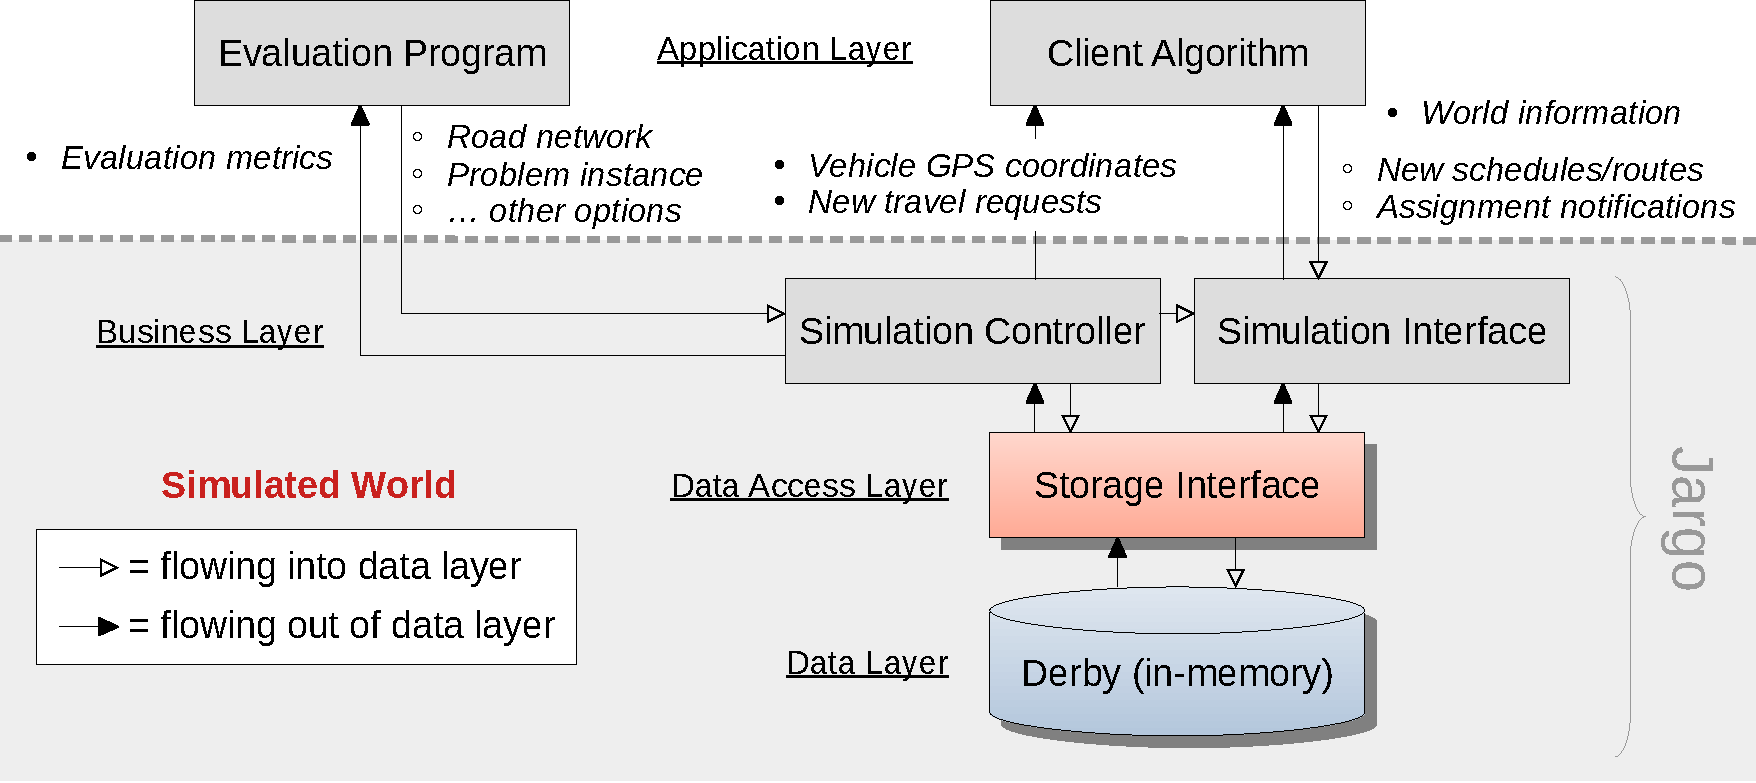
\includegraphics[width=120mm]{src/fig/storage-fig}
\caption{Storage interface and data layer within the Jargo stack.}
\label{fig:storage}
\end{figure}

The storage interface is developed using the
Noweb\footnote{\url{https://www.cs.tufts.edu/~nr/noweb/}} literate
programming\footnote{\url{http://literateprogramming.com/}} tool.  This file
({\tt{}src/storage.nw}) is the source for both the documentation
({\tt{}doc/storage.tex}) and the Java code (Storage.java)\footnote{See the
{\tt{}Makefile} for build details.}.

\begin{figure}
\adjustbox{scale=0.85}{
\begin{minipage}[t]{0.40\textwidth}
\hi{Utilities}
\nwfilename{src/storage.nw}\nwbegincode{1}\sublabel{NW15FRcE-4PbjF-1}\nwmargintag{{\nwtagstyle{}\subpageref{NW15FRcE-4PbjF-1}}}\moddef{\code{}Storage\edoc{} public methods~{\nwtagstyle{}\subpageref{NW15FRcE-4PbjF-1}}}\endmoddef\nwalsodefined{\\{NW15FRcE-4PbjF-2}\\{NW15FRcE-4PbjF-3}}\nwused{\\{NW15FRcE-3TAldU-1}}
\LA{}Load backup~{\nwtagstyle{}\subpageref{NW15FRcE-b3Hn1-1}}\RA{}
\LA{}Save backup~{\nwtagstyle{}\subpageref{NW15FRcE-2OKmqF-1}}\RA{}
\LA{}Print SQL exception~{\nwtagstyle{}\subpageref{NW15FRcE-31QNBg-1}}\RA{}
\LA{}Compute haversine~{\nwtagstyle{}\subpageref{NW15FRcE-1XfngC-1}}\RA{}
\LA{}Print user~{\nwtagstyle{}\subpageref{NW15FRcE-3sWW32-1}}\RA{}
\LA{}Print path~{\nwtagstyle{}\subpageref{NW15FRcE-3QvbXQ-1}}\RA{}
\LA{}Print route~{\nwtagstyle{}\subpageref{NW15FRcE-2sTsm3-1}}\RA{}
\LA{}Print schedule~{\nwtagstyle{}\subpageref{NW15FRcE-45oGvT-1}}\RA{}
\nwendcode{}\nwbegindocs{2}\nwdocspar
\end{minipage}
\begin{minipage}[t]{0.40\textwidth}
\hi{Write Methods}
\nwenddocs{}\nwbegincode{3}\sublabel{NW15FRcE-4PbjF-2}\nwmargintag{{\nwtagstyle{}\subpageref{NW15FRcE-4PbjF-2}}}\moddef{\code{}Storage\edoc{} public methods~{\nwtagstyle{}\subpageref{NW15FRcE-4PbjF-1}}}\plusendmoddef
\LA{}Update edge speed~{\nwtagstyle{}\subpageref{NW15FRcE-3SpUqj-1}}\RA{}
\LA{}Add new request~{\nwtagstyle{}\subpageref{NW15FRcE-4ISWm4-1}}\RA{}
\LA{}Add new server~{\nwtagstyle{}\subpageref{NW15FRcE-IYVQQ-1}}\RA{}
\LA{}Update server route~{\nwtagstyle{}\subpageref{NW15FRcE-4VFddh-1}}\RA{}
\LA{}Update server schedule~{\nwtagstyle{}\subpageref{NW15FRcE-43w3hJ-1}}\RA{}
\LA{}Update server add to schedule~{\nwtagstyle{}\subpageref{NW15FRcE-y828a-1}}\RA{}
\LA{}Update server remove from schedule~{\nwtagstyle{}\subpageref{NW15FRcE-lMiTm-1}}\RA{}
\nwendcode{}\nwbegindocs{4}\nwdocspar
\end{minipage}
\begin{minipage}[t]{0.40\textwidth}
\hi{Read Methods}
\nwenddocs{}\nwbegincode{5}\sublabel{NW15FRcE-4PbjF-3}\nwmargintag{{\nwtagstyle{}\subpageref{NW15FRcE-4PbjF-3}}}\moddef{\code{}Storage\edoc{} public methods~{\nwtagstyle{}\subpageref{NW15FRcE-4PbjF-1}}}\plusendmoddef
\LA{}Query ridesharing user~{\nwtagstyle{}\subpageref{NW15FRcE-3isdeu-1}}\RA{}
\LA{}Query queued requests~{\nwtagstyle{}\subpageref{NW15FRcE-3AGrxZ-1}}\RA{}
\LA{}Query all server locations~{\nwtagstyle{}\subpageref{NW15FRcE-rvb17-1}}\RA{}
\LA{}Query active server locations~{\nwtagstyle{}\subpageref{NW15FRcE-3UaQCb-1}}\RA{}
\LA{}Query routes~{\nwtagstyle{}\subpageref{NW15FRcE-1AprqI-1}}\RA{}
\LA{}Query schedules~{\nwtagstyle{}\subpageref{NW15FRcE-3yA8FQ-1}}\RA{}
\LA{}Query current load~{\nwtagstyle{}\subpageref{NW15FRcE-aKbeg-1}}\RA{}
\LA{}Query various metrics~{\nwtagstyle{}\subpageref{NW15FRcE-1Ang64-1}}\RA{}
\LA{}Query custom statement~{\nwtagstyle{}\subpageref{NW15FRcE-2FtqIZ-1}}\RA{}
\nwendcode{}\nwbegindocs{6}\nwdocspar
\end{minipage}
}
\caption{Storage interface public methods.}
\label{fig:methods}
\end{figure}

\subsection{Motivation}
\label{sec:motivation}
Ridesharing can be formulated as a decision problem where the objective is to
determine the optimal customer-to-vehicle assignments. Optimizing a single
assignment produces a \emph{local optima} whereas optimizing the aggregated
objective over all assigments in the span of a ridesharing scenario produces
the \emph{global optima}. The global optima answers questions that are of
interest to various stakeholders, such as what is the minimum fleet size needed
for an $n$\% assignment rate or what is the maximum profit achievable in a day.

To evaluate the \emph{quality} of a ridesharing algorithm (some might say the
\emph{quality of the solution} produced by the algorithm) is to measure the
value of the objective that the algorithm can achieve over the ridesharing
scenario. A high-quality algorithm achieves near the global optima whereas a
low-quality algorithm does not.  Quality of a ridesharing algorithm is
difficult to evaluate for three reasons.
\begin{enumerate}
\item \hi{Assignment Dependence.} Assignments are not independent of each
other. If a vehicle is initially assigned to a particular customer, it may be
ineligible for some future customer due to capacity and time window
constraints. This dependence means that assignments cannot be evaluated
sequentially in isolation but must be evaluated as part of a broader system.
\item \hi{Stochastic Processes.} Stochastic processes become important over the
span of a scenario.  Travel times in the road network are uncertain due to
traffic and vehicle breakdowns. Travel routes are also uncertain, if the
vehicles are non-autonomous, because human drivers can make mistakes.  If a
vehicle is initially assigned to a customer in an area that is susceptible to
traffic or difficult to navigate, it may be ineligible for some future customer
due to time window constraints. These processes cannot be ignored because they
can affect the downstream assignments.
\item \hi{Real-Time Requests.} A ridesharing algorithm's processing time
affects downstream assignments due to the real-time nature of ridesharing
requests. As a simple example, consider an algorithm that processes requests at
a rate slower than they appear. Over time, later requests may never get
processed even if valid assignments exist for them.
\end{enumerate}

The above items are all features of ridesharing in the real world.  Thus to
evaluate quality, ridesharing algorithms can be tested on actual vehicles and
customers (Figure~\ref{fig:physical}), but this method is expensive, slow to
deploy, and out of reach for most researchers. Controlled studies to determine
the effect of certain parameters, such as presence and absence of traffic, on
algorithm quality are also difficult or impossible to perform. In contrast,
testing algorithms on a simulated environment is inexpensive, fast to deploy,
readily accessible, and controllable. The challenge then becomes to design an
environment that can simulate these items.

\begin{figure}[h]
\centering
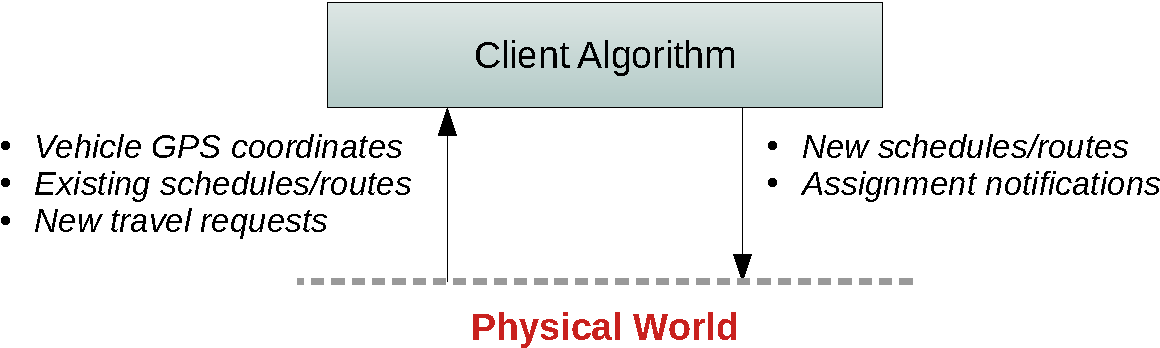
\includegraphics[width=100mm]{src/fig/physical}
\caption{Evaluating algorithms on physical vehicles and customers is expensive,
    slow to deploy, and out of reach for most researchers.}
\label{fig:physical}
\end{figure}

Jargo is the name of our environment for evaluating the quality of ridesharing
algorithms. It captures assignment dependence by simulating real-time motion of
vehicles and capacity, and it simulates stochastic processes by perturbing
route segment durations and locations. To simulate real-time, it executes a
ridesharing algorithm in parallel alongside new requests so that an algorithm
can be running while requests are arriving. The present document concerns the
storage interface, used by Jargo's simulation engine to read and write data
describing the state of the environment. The storage interface (more precisely
the underlying data model) is responsible for guaranteeing the integrity of the
state, in other words that impossible circumstances in the real world do not
end up in the simulation data. The following is an explanation of how the data
is organized, beginning with a description of physical ridesharing
(\S\ref{sec:ridesharing-systems}), then the mathematical model to describe
physical ridesharing (\S\ref{sec:ridesharing-formulation}), and finally the
SQL schema to store the state data (\S\ref{sec:ridesharing-data-model}).  Those interested
in the storage interface code can skip directly to
\S\ref{sec:implementation-overview}.

\subsection{Ridesharing Systems}
\label{sec:ridesharing-systems}
To determine the best way to organize the state data, we first start with
examining real-world ridesharing systems.  Ridesharing involves the
\emph{users} and the \emph{rules} governing their behavior. The users can be
classified into four types, shown in Table~\ref{tab:user-types}.
\begin{table}[h]
\centering
\small
\caption{Types of ridesharing users.}
\label{tab:user-types}
\begin{tabular}{|l|l|}
\hline
Type   & Description \\
\hline
Type 1 & Single customer traveling alone \\
Type 2 & Group of customers traveling together \\
\hline
Type 3 & Ridesharing vehicle with a predefined final
    destination\footnote{For example a carpooling vehicle.} \\
Type 4 & Taxi-like vehicle continually serving customers without an
    explicit destination of its own\footnote{A Type 4 vehicle could have an
    eventual destination, for example a refueling station; but if the latest
    acceptable arrival time is outside the time span of the ridesharing
    scenario of interest, the destination is not considered. Otherwise, the
    vehicle would be classified as Type 3.}. \\
\hline
\end{tabular}
\caption{Ridesharing user properties.}
\label{tab:user-properties}
\begin{tabular}{|c|p{140mm}|}
\hline
Label & Description \\
\hline
P1 & \hi{Load.} Each user has a non-zero \emph{load}, indicating a
number of needed seats. For Type 1 users the load is 1, indicating they only
need a single seat. For Type 2 users the load exceeds 1. For Type 3 and Type 4
users the load is negative, indicating they have an availability of seats. \\
\hline
P2 & \hi{Origin and Destination.} Each user has an \emph{origin} and a
\emph{destination}, except for Type 4 users that only have an origin.  For Type
1 and Type 2, the origin indicates the initial location of the customer
and the destination indicates the desired final location.  For Type 3, the
origin and destination indicate where the vehicle's ridesharing service begins
and ends.\\
\hline
P3 & \hi{Time Window.} Each user has an \emph{early time} and a
\emph{late time}, together forming the user's \emph{time window}. For a Type 1
or Type 2 customer, the time window gives the desired departure time from the
origin and the desired arrival time at the destination.  For a Type 3 or Type 4
vehicle, the time window gives the time when service begins and the latest time
that service can end. The early time precedes the late time.\\
\hline
\end{tabular}
\caption{Rules bounding user behavior.}
\label{tab:user-rules}
\begin{tabular}{|c|p{140mm}|}
\hline
Label & Description \\
\hline
P4 & \hi{Motion.} Users are bound to a network of roads, for
example the streets of a city. Only vehicles may directly travel along the
roads, whereas customers must be serviced by a vehicle. Both customers and
vehicles may enter the system at any time and anywhere.\\
\hline
P5 & \hi{Pick-ups and Drop-offs.} For a vehicle to service a customer, it
must first travel to the customer's origin to pick up the customer, and then to
the customer's destination to drop off the customer, in that order. The
customer enters the vehicle during the pick-up and exits the vehicle during the
drop-off. These visits must occur within the customer's time window\footnote{We
limit our scope to the typical case where a customer is served by only one
vehicle (no transfers).}.\\
\hline
P6 & \hi{Vehicle Seats.} When a customer enters a vehicle, the customer
occupies a number of seats equal to the customer's load. When it exits the
vehicle, it relinquishes the seats. At no time can the number of occupied seats
exceed the number of available seats in a vehicle.\\
\hline
P7 & \hi{User States.} A customer can be in one of three states at any
time: \emph{waiting} for pick-up; \emph{in-transit} following a pick-up but
before the drop-off; or \emph{arrived} at destination. A vehicle can be either
\emph{in-service} or \emph{out-of-service}.\\
\hline
\end{tabular}
\end{table}
We use the term \emph{customer} to refer to both Type 1 and Type 2 users, and
the term \emph{vehicle} to refer to both Type 3 and Type 4 users.
Physical users have the properties in Table~\ref{tab:user-properties} and obey
the rules in Table~\ref{tab:user-rules}.

\subsection{Ridesharing Formulation}
\label{sec:ridesharing-formulation}
We can now try to mathematically describe the system.  Users can naturally be
described by a set of values for their P1--P3 properties.  Each vehicle can
also be associated with a sequence of values describing its past and future
motion (P4); a set of values indicating when and where pick-ups and drop-offs
have occurred (P5); and a value to indicate the number of available seats at
any given time (P6). Each customer can be associated with a value indicating
its state (P7). Moreover, the ridesharing setting, namely the road network, can
be described using sets of values indicating coordinates and distances in the
network.

Now that we know what values we have, we can try to organize the data into variables
and constants and write equations to explain the relationships. If we
organize the data into \emph{relations}, we can use selection and projection
when we write the equations. These operations will turn out to be useful for
formalizing certain concepts such as pick-up and drop-off times for a customer
or the cruising and service distance for a vehicle.

\subsubsection*{Relations}
\label{sec:relations}
The following briefly overviews the concept of relations and introduces some
notation.
Relations can be defined in terms of \emph{sequences} and \emph{tuples}.
A sequence is an ordered list of elements.
We will write the integer sequence from $i$ to
$j$ as $i..j$. The sequence
$$(a_i)_{i\in 1..n}=a_1,a_2,...,a_{n-1},a_n$$
will be written $a_1..a_n$ or simply $a$ (without any subscript).
The number of elements in $a$ is called the \emph{length}
of $a$ and is expressed as $|a|$.
A copy $b$ of sequence $a$ but with some elements removed is called
a \emph{subsequence}.
Sequence $b$ is called a \emph{substring} of $a$
only if some $k$ exists such that $$b=a_{1+k}..a_{|b|+k},$$
in other words the elements in $b$ form a contiguous subsequence of $a$.
We call
sequence $a$ a \emph{tuple} if each element of $a$ is labeled. A
labeled element is called a \emph{component}.
A function mapping an element based on its position in the tuple to a label
is called a \emph{labeling scheme}.
Each component also has a \emph{domain} from which the component takes its value,
for example the set of real numbers.
A tuple of length $m$ is called an $m$-tuple. A 2-tuple is called a
\emph{pair}.
A tuple definition will be written as its labels surrounded by parentheses with the
domains given. Label names will be written in \texttt{typewriter} script
to avoid confusion with positional indices.

\begin{example}
\label{ex:tuple}
The sequence $a=a_\texttt{x},a_\texttt{y}$
is a 2-tuple with components named \texttt{x} and \texttt{y}.
The labeling
scheme for $a$ maps $1\rightarrow \texttt{x}$ and $2\rightarrow \texttt{y}$, with the
integers $1$ and $2$ referring to the position of the elements. A possible definition for
$a$ could be $a:=(\texttt{x},\texttt{y}),
a_\texttt{x}\in\mathbb{R}, a_\texttt{y}\in\{\textrm{cat},\textrm{dog}\}.$
\end{example}

A set of unique $m$-tuples with the same labeling scheme is called
an \emph{$m$-ary relation}, or simply relation.
Two operators can be applied onto relations\footnote{Our model is not concerned with joins.}.
The \emph{selection operator} $\sigma_P(R)$ is a function that returns a subset
$R'\subseteq R$ such that predicate $P(R'_i)$ is true for each tuple $R'_i\in R'$.
The \emph{projection} operator $\pi_L(R)$ is a function that returns a copy
$R'$ of $R$ such that each tuple $R'_i\in R'$ is distinct, and only components
with a label in set $L$ are included.

Observe that an $m$-tuple is an $m$-ary relation with one element.
The projection operator thus naturally applies to tuples. For instance, see that for
$R=R_\texttt{x},R_\texttt{y}:=(\texttt{x},\texttt{y}),$
the $\texttt{x}$ component is extracted with
$R_\texttt{x}=\pi_\texttt{x}(R)$
and the $\texttt{y}$ component is extracted with
$R_\texttt{y}=\pi_\texttt{y}(R)$.

\subsubsection{Setting}
\label{sec:setting}
Now we begin to assign variables and constants to the ridesharing
system, starting with the setting.

\hi{Time.} Time is considered to be a positive integer $1\leq t\leq H$.  A
\emph{time horizon} $H$ is introduced to bound the system.

Time will occasionally need to be operated on.  Times cannot be added, and only
a later (greater) time can subtract an earlier (lesser) time.  The difference
is called a \emph{duration}, represented by the symbol $\delta$.  Durations can
add and subtract each other to get new durations, and times can also add and
subtract durations to get new times.

\hi{Road Network.}
The road network is considered to be a directed graph $\mathcal{G}(\mathcal{V},\mathcal{E})$.
Vertices in $\mathcal{V}$ represent points along roads in the network.
A function ${V:\mathcal{V}\rightarrow \mathbb{R}^2}$ maps vertices to
$2$-dimensional latitude and longitude coordinates in the real world.
An inverse function can be used to map-match customers and vehicles to vertices.
Edges in $\mathcal{E}$ represent road segments. The pair $(a,b)\in
\mathcal{V}^2, a\neq b$ exists in $\mathcal{E}$ only if physical traffic flows from
$V(a)$ to $V(b)$, and for all $c\in \mathcal{V}\setminus\{a,b\}$ no traffic flows from
$V(a)$ to $V(c)$ and from $V(c)$ to $V(b)$.
A function ${d:\mathcal{E}\rightarrow\mathbb{R}_{>0}}$ maps edges to positive real weights
corresponding to distance along the edge. See that the
shortest-path distances between the pairs among any three vertices satisfies the
triangle inequality.

\begin{figure}[h]
\centering
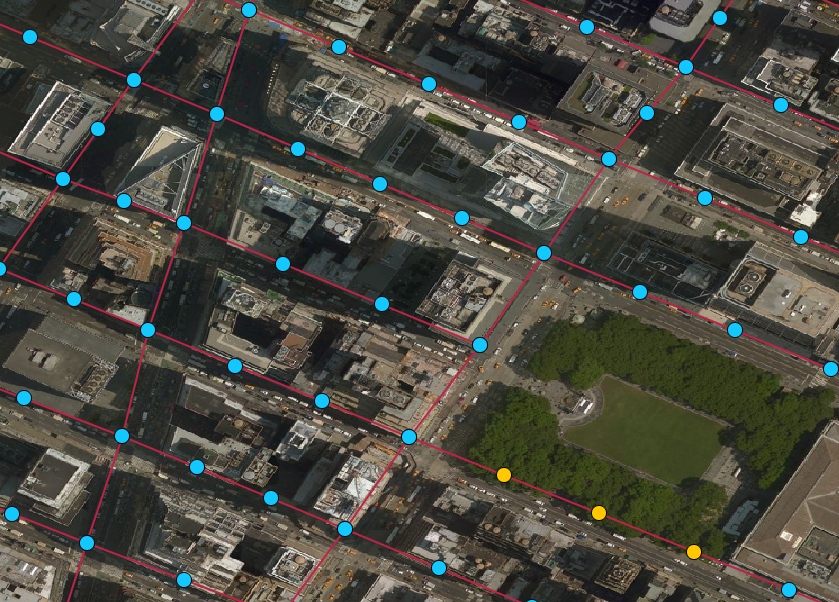
\includegraphics[width=0.8\textwidth]{src/fig/road}
\caption{Portion of a road network graph showing edges (red lines) and vertices
(blue circles) overlayed on top of Manhattan (QGIS 2.18.16, Bing Aerial).
Vertices do not have to be at an intersection (orange circles, lower right).}
\label{fig:road}
\end{figure}

\hi{Paths.}
A path $p=(p_i)_{i\in 1..n}=p_1..p_n$ is a sequence of $n$ vertices
such that any two adjacent vertices are an edge, or $(p_i,p_{i+1})\in \mathcal{E}$ for
$i\in 1..(n-1)$.
A vertex or edge can appear multiple times in a path.
The \emph{path distance} is
$$\sum_{i=1}^{n-1} d(p_i, p_{i+1}).$$
Path $p$ is a \emph{shortest path} only if it minimizes the distance out of all
possible paths from $p_1$ to $p_n$.
Multiple shortest paths are possible.

\hi{Waypoints.}
Waypoints are used to describe points in time as well as space.
A waypoint is a tuple $(\texttt{t},\texttt{v})$, with the
domain of $\texttt{t}$ as $1..H$ and the domain of $\texttt{v}$ as
$\mathcal{V}$. Waypoints can be labeled in a way that will be
discussed later.

\hi{Routes.}
Routes are formed by a sequence of waypoints. A route
$w=(w_i)_{i\in 1..n}=w_1..w_n=(t_1,v_1)..(t_n,v_n)$
is defined as a sequence of $n$ waypoints such that
$t_1..t_n$ is strictly increasing and $v_1..v_n$ is a path.
%In other words it is a binary relation on time and $\mathcal{V}$.
In the spatial dimension, function
$$D(w)=\sum_{i=1}^{n-1}d(\pi_\texttt{v}(w_i),\pi_\texttt{v}(w_{i+1}))$$
gives the \emph{route distance}, analogous to path distance.
% Abandoned: wordy. Projection $\pi_\texttt{v}(w_i)$ returns the vertex component of waypoint $w_i$.
In the time dimension, function
$$\delta(w)=\pi_\texttt{t}(w_n)-\pi_\texttt{t}(w_1)$$
gives the \emph{route duration}.
%The \emph{distance} of $w$ is $D(\pi_\texttt{v}(w))$.
%The \emph{duration} of $w$ is $t_n$.
Given a time $t$,
\begin{align*}
w_{\leq t}=\textrm{sort}(\sigma_{\texttt{t}\leq t}(w))\quad\textrm{and}\quad
w_{>t}=\textrm{sort}(\sigma_{\texttt{t}>t}(w))
\end{align*}
give the \emph{traveled route} denoted $w_{\leq t}$, and the \emph{remaining
route} denoted $w_{>t}$. As the selection operator imposes no ordering on the resulting
set, a $\textrm{sort}(...)$ function is introduced to
sort a set of waypoints by time in ascending order, returning a sequence.
% From now on, any selection or projection on time is assumed to be sorted
% in this manner.
For two adjacent waypoints $w_i$ and~$w_{i+1}$, function
$$\nu(w_i,w_{i+1})=\frac{d(\pi_\texttt{v}(w_i),\pi_\texttt{v}(w_{i+1}))}
{\pi_\texttt{t}(w_{i+1})-\pi_\texttt{t}(w_i)}$$ gives the
\emph{waypoint rate}, or more intuitively the \emph{speed}.
% The unit of speed depends on the units of $d$ and time and do not have to be
% a physical velocity, such as meters per second.
As $d$ only applies to edges, $\nu$ only applies to adjacent waypoints.
Speeds can be bounded above by a value $\nu^\textrm{max}(v_i,v_{i+1})$ on each edge,
for example to describe road speed limits.
%The speed limit can be different
%on different edges, but to simplify the notation, let $\nu_{max}$ denote the limit for any edge.
%Note that duration $t_n$ and distance $D(\pi_\texttt{v}(w))$ are
%convertible through the speeds along each of the edges.

\subsubsection{Requests and Servers}
\label{sec:requests-and-servers}
Now we define the requests and servers.
The basic entity representing a ridesharing participant is the \emph{user}.  A
user is classified as a \emph{request} if it represents a Type~1 or Type~2
customer, or classified as a \emph{server} if it represents a Type~3 or Type~4
vehicle. As only vehicles can move about (P4), only servers are associated with
routes in order to describe the motions. Later, \emph{schedules} describing
pick-up and drop-off events will be defined on the routes.

\hi{User Relation}
A user $u$ is a 5-tuple defined by
${u:=(\texttt{q},\texttt{e},\texttt{l},\texttt{o},\texttt{d})}$.  The
\texttt{q} component corresponds to the user load; the \texttt{e} and
\texttt{l} components correspond to the user early and late times; the
\texttt{o} and \texttt{d} components correspond to the user origin and
destination.
From P1--P4, the domain of \texttt{q} is the non-zero integers; the domain of \texttt{e} is
$1..(H-1)$ and the domain of \texttt{l} is $(u_\texttt{e}+1)..H$; the domains
of \texttt{o} and \texttt{d} are both $\mathcal{V}$.
For a Type 4 vehicle, the destination can be set to a dummy vertex with edge
weight equal to 0 to every other vertex in the road network.

The set of all users forms the 5-ary relation $\mathcal{U}$, called
the \emph{user relation}.
The set
$\mathcal{U}_\texttt{o}=\pi_\texttt{o}(\mathcal{U})$ contains all origins and
$\mathcal{U}_\texttt{d}=\pi_\texttt{d}(\mathcal{U})$ contains all destinations.
From P1, a user can be classified as either a request or a server based on its load.

From now on as a convenience, the notation $d_u$ will be used to denote the distance of the
shortest path from $u_\texttt{o}$ to $u_\texttt{d}$ on graph $\mathcal{G}$, and
the notation $\delta_u$ will be used to denote the shortest travel duration
along $d_u$ using the speed limits $\nu^\textrm{max}$ along the shortest-path edges.

\hi{Requests.}
A request represents a Type 1 or Type 2 customer.
According to P1,
relation $\mathcal{R}\subseteq\mathcal{U}$,
$$\mathcal{R}=\sigma_{\texttt{q}>0}(\mathcal{U}),$$
% Abandoned: $$\mathcal{R}=\{r\in \mathcal{U}\mid r_\texttt{q}>0\},$$
forms the set of all requests by taking users with positive loads. The set
$\mathcal{R}_\texttt{o}=\pi_\texttt{o}(\mathcal{R})$ is the set of all request origins and
$\mathcal{R}_\texttt{d}=\pi_\texttt{d}(\mathcal{R})$ is the set of all request destinations.
%Abandoned: "corresponding" vertices
%Abandoned: Vertex $v$ is a \emph{pickup} if $v\in \mathcal{R}_o$ and it is a
%\emph{dropoff} if $v\in \mathcal{R}_d$.

\hi{Servers.}
Likewise, a server represents a Type 3 or Type 4 vehicle.
From P1, the relation $\mathcal{S}=\mathcal{U}\setminus\mathcal{R}$, or
$$\mathcal{S}=\sigma_{\texttt{q}<0}(\mathcal{U}),$$
% Abandoned: $$\mathcal{S}=\{s\in \mathcal{U}\mid s_\texttt{q}<0\},$$
forms the set of all servers. The set
$\mathcal{S}_\texttt{o}=\pi_\texttt{o}(\mathcal{S})$ is the set of all server origins and
$\mathcal{S}_\texttt{d}=\pi_\texttt{d}(\mathcal{S})$ is the set of all server destinations.
%Abandoned: The vehicle has a speed $\nu(a,b)$ along edge $(a,b)$. For
%simplicity, denote the speed as $\nu$ for all vehicles and all edges.

\hi{Routes and Schedules}
To encode vehicle motions, each server $s\in\mathcal{S}$ is associated with a
route and a schedule.  A server's route is a representation of the corresponding
vehicle's motion through the road network while a server's schedule
encodes the times and locations of customer pick-ups and drop-offs.
The schedule describes the events along the route and not any new motion,
therefore it is a subsequence of the server's route.

\hi{Server Routes.}
Let $w$ be the route for server $s$. As time
advances, the traveled route $w_{\leq t}$ encodes the server's past
motion while the remaining route $w_{>t}$ encodes the future motion.
From P2 and P3, the route is subject to two rules:
\begin{enumerate}
\item[R1.] The time component of the first waypoint equals the server's early time,
  and the time component of the last waypoint is not greater than the server's late time,
  or $\pi_\texttt{t}(w_1)=s_\texttt{e}$ and $\pi_\texttt{t}(w_{|w|})\leq s_\texttt{l}$;
\item[R2.] The vertex components of the first and last waypoints equal the
  server's origin and destination respectively, or
  $\pi_\texttt{v}(w_1)=s_\texttt{o}$ and $\pi_\texttt{v}(w_{|w|})=s_\texttt{d}$.
\end{enumerate}

\hi{Server Schedules.}
A server's schedule
$$b=(b_j)_{j\in 1..m}=(w_{i_j})_{j\in 1..m}=(t_{i_1},v_{i_1})..(t_{i_m},v_{i_m})$$
is a subsequence of the server's route $w$, with $m\leq |w|$ waypoints.
First:
\begin{enumerate}
\item[R3.] The first and last waypoints $b_1$ and $b_m$ equal the first and last
waypoints of $w$, or ${b_1=w_1}$ and ${b_m=w_{|w|}}$.
\end{enumerate}
This rule will help later when defining departure and arrival times.
Second, from P5:
\begin{enumerate}
\item[R4.] For each waypoint $b_j$ for $j\in 2..(m-1)$, the vertex component is either a
request origin or request destination, or $\pi_\texttt{v}(b_j)\in
\mathcal{R}_\texttt{o}\cup\mathcal{R}_\texttt{d}$.
\end{enumerate}
In other words, each entry or exit must occur at a customer origin or destination.

A schedule formalizes the notion of shared travel with other users, as
multiple entries and exits can overlap within the same server route.
At time $t$, the \emph{traveled schedule} denoted $b_{\leq t}$ encodes the past entries and exits and is given by
$\sigma_{\texttt{t}\leq t}(b)$. Likewise, the \emph{remaining schedule} denoted
$b_{>t}$ encodes the future entries and exits and is given by $\sigma_{\texttt{t}>t}(b)$.

\hi{Schedule Labels.}
Each waypoint in schedule $b$ has a set of labels in order to identify which
customers are entering and exiting the vehicle at the waypoint's time and location.
A labeling scheme can be applied to $b$ to determine each of the labels. The
set of all possible labels depends on the locations of the waypoints. Let
$$\mathcal{R}'=\sigma_{\texttt{o}\in\pi_\texttt{v}(b)\lor \texttt{d}\in\pi_\texttt{v}(b)}(\mathcal{R})$$
%Abandoned: $$\mathcal{R}'=\{r\in \mathcal{R}\mid
%     r_\texttt{o}\in\pi_\texttt{v}(b)\vee r_\texttt{d}\in\pi_\texttt{v}(b)\}$$
give the set of requests whose origin or destination is found
in at least one waypoint in $b$. The labeling scheme
\begin{equation*}
L:b\rightarrow \mathbb{P}(\mathcal{R}'\cup\{s\})
\end{equation*}
maps elements of $b$ to elements of the power set of $\mathcal{R}'\cup\{s\}$.
By using the power set $\mathbb{P}$,
a waypoint can have multiple labels, representing the case where multiple customers
enter or exit the vehicle at the waypoint.
The labeling scheme is subject to the following labeling rules:
\begin{enumerate}
\item[R5.] No waypoint can be labeled with $r\in\mathcal{R}'$ if a schedule for another server
already contains waypoints labeled with $r$;
\item[R6.] A waypoint $b_j\in b$ can be labeled with $r$ only if
$\pi_\texttt{v}(b_j)=r_\texttt{o}$ or $\pi_\texttt{v}(b_j)=r_\texttt{d}$;
\item[R7.] If $b_j$ is to be labeled with $r$ and $\pi_\texttt{v}(b_j)=r_\texttt{o}$, then
a second waypoint $b_{j'}$ such that $j'>j$ and
$\pi_\texttt{v}(b_{j'})=r_\texttt{d}$ must also be labeled with $r$;
\item[R8.] The time components of $b_j$ and $b_{j'}$ must be within request $r$'s time window,
formally $r_\texttt{e}\leq \pi_\texttt{t}(b_j)$ and $\pi_\texttt{t}(b_{j'})\leq r_\texttt{l}$;
\item[R9.] The number of waypoints labeled with $r$ must be exactly 0 or 2;
\item[R10.] The first and last waypoints must contain the schedule's server $s$
in their labels, and no other waypoint can be labeled with $s$.
\end{enumerate}
Rules R5--R9 express P5.  Rule R10 can be interpreted to mean that a vehicle
must ``serve itself'' at its own origin and destination.  This last rule
helps to define later concepts.

\hi{Server Relation}
By combining the routes, schedules, and labels into
a set of $(\texttt{s},\texttt{t},\texttt{v},\texttt{L})$ tuples, a
4-ary relation $\mathcal{X}$ can be formed. This relation is called the
\emph{server relation} and as will be shown soon, it is the basis for computing many common ridesharing metrics.
Each tuple associates the waypoint in the \texttt{t} and \texttt{v} components with the server
in the \texttt{s} component, along with the labels in the \texttt{L} component.
% The domain of $\texttt{s}$ is $\mathcal{S}$; the domain of $\texttt{t}$ is
% $1..H$; the domain of $\texttt{v}$ is $\mathcal{V}$; the domain of $\texttt{L}$
% is the power set $\mathbb{P}(\mathcal{U})$.

A server's route can be recovered by extracting \texttt{t} and \texttt{v}
components and sorting by time, or formally for a given server $s$, its route
is given by
$$W(\mathcal{X},s)=\textrm{sort}(\pi_{\texttt{t},\texttt{v}}(\sigma_{\texttt{s}=s}(\mathcal{X}))).$$
Similarly, a server's schedule can be recovered by
extracting only those waypoints that are labeled, formally
$$B(\mathcal{X},s)=\textrm{sort}(\pi_{\texttt{t},\texttt{v}}(\sigma_{\texttt{s}=s\land |\texttt{L}|>0}(\mathcal{X}))).$$

The server relation can be used to define the remaining physical concepts, P6 and P7.

\hi{Request Status.}
Given a request $r$, the function
\begin{equation}
\label{eq:status}
\textrm{status}(\mathcal{X},r,t)=|\sigma_{\texttt{t}\leq t\land
r\in\texttt{L}}(\mathcal{X})|
\end{equation}
gives the count of the tuples labeled with $r$
before or on a given time. From the labeling rules, the count can be only 0, 1,
or 2. See that these counts correspond to request waiting, in-transit, and arrived states
from P7, respectively.

Given a server $s$, knowing the in-transit requests for $s$ can be useful for
pricing and other rider-related
metrics. %~\cite{DBLP:conf/sigmod/ChengX017,DBLP:conf/dexa/ShiLZG17,DBLP:conf/ijcai/SantosX13}.
These requests can be easily found by
$$\mathcal{Q}(\mathcal{X},s,t)=\{r\in\mathcal{R}\mid\textrm{status}(\mathcal{X},r,t)=1
\land\pi_\texttt{s}(\sigma_{r\in\texttt{L}}(\mathcal{X}))=s\}.$$

\hi{Load Burden.}
The \emph{load burden} on $s$ can be computed using the in-transit requests by
\begin{equation}
\label{eq:load}
Q(\mathcal{X},s,t)=\sum_{r\in\mathcal{Q}(\mathcal{X},s,t)}r_\texttt{q}.
\end{equation}
From P6, server routes are subject to the additional rule:
\begin{enumerate}
\item[R11.] $Q(\mathcal{X},s,t)\leq -s_\texttt{q}$ must be true for all $s$ and $t$.
\end{enumerate}

\subsubsection{Ridesharing Metrics}
\label{sec:ridesharing-metrics}
As a benefit from using relations, a variety of metrics can now be measured by
simple operations on $\mathcal{U}$ and $\mathcal{X}$.  The following lists
common metrics found in existing ridesharing studies, but others may be possible.

\hi{Assignments.}
Server $s$ is said to be \emph{assigned to} request $r$ at time $t$ only if
$\textrm{status}(\mathcal{X},r,t)=2$. That is, the request's status is arrived at time $t$.
The set of $(s,r)$ pairs
where this property is true is called the set of \emph{assignments}, formally
\begin{equation}
\label{eq:assignments}
\textit{assignments }A(\mathcal{X},t)=
\{(s,r)\in\mathcal{S}\times \mathcal{R} \mid \textrm{status}(\mathcal{X},r,t)=2\}.
\end{equation}
Using the assignments,
\begin{align}
\label{eq:assigned-requests}
\textit{assigned requests }R^\textrm{ok}(\mathcal{X},t)&=\pi_\texttt{r}(A(\mathcal{X},t))\textrm{, and}\\
\label{eq:unassigned-requests}
\textit{unassigned requests }R^\textrm{ko}(\mathcal{X},t)&=\mathcal{R}\setminus\mathcal{R}^\textrm{ok}(\mathcal{X},t).
\end{align}
The server assigned to $r$ can be obtained with
\begin{equation}
S(\mathcal{X},r,t)=\{s\in\mathcal{S}\mid\textrm{status}(\mathcal{X},r,t)=2\},
\end{equation}
guaranteed to return only one server due to R5.
Likewise, the set of requests assigned to $s$ can be obtained with
\begin{equation}
R(\mathcal{X},s,t)=\{r\in\mathcal{R}\mid\textrm{status}(\mathcal{X},r,t)=2\}.
\end{equation}

\hi{Service rate.}
The \emph{service rate} is the number of assigned requests over the number of all requests, or
\begin{equation}
\label{eq:service-rate}
\textit{service rate }\mu(\mathcal{X},t)=\frac{|R^\textrm{ok}(\mathcal{X},t)|}{|\mathcal{R}|}.
\end{equation}

\hi{Distances.}
The \emph{base distance} is the sum of the shortest-path distances for all users, or
\begin{equation}
\label{eq:base-distance}
\textit{base distance }D^\textrm{base}(\mathcal{U})=\sum_{u\in U}d_u.
\end{equation}
The \emph{travel distance} for one server $s$ is the distance of its route,
$D(W(\mathcal{X},s))$,
and the \emph{travel duration} can be found with
$\delta(W(\mathcal{X},s))$.

For a server with route $w$, travel distance $D(w)$ can be partitioned into
\emph{cruising distance} $D_0(w)$ and
\emph{service distance} $D_1(w)$.
The cruising distance sums the distance along portions where the load burden is zero.
The service distance sums the distance along portions of $w$ where the
load burden is non-zero.
Formally, partition $w$ into a set of substrings $\Omega(w)$ such that each waypoint
in $w$ is a member of exactly one substring and that for all substrings $\omega\in \Omega$,
\begin{align}
\label{eq:slack}\textrm{either }Q(\mathcal{X},s,t)&=0\textrm{ is true for all }t\in \pi_\texttt{t}(\omega),\\
\label{eq:block}\textrm{or }Q(\mathcal{X},s,t)&>0\textrm{ is true for all }t\in \pi_\texttt{t}(\omega).
\end{align}
%Observe that Eqs.~\ref{eq:slack}~and~\ref{eq:block}
%formalize concepts similar to the intuitive
%\emph{slack periods} and \emph{schedule blocks} in~\cite{jaw:1986}.
The equations can be used to partition $\Omega(w)$ into two subsets,
\begin{align*}
\Omega_0(w)&=\{\omega\in \Omega(w)\mid \omega\textrm{ satisfies Eq.~\ref{eq:slack}}\}\textrm{ and }\\
\Omega_1(w)&=\{\omega\in \Omega(w)\mid \omega\textrm{ satisfies Eq.~\ref{eq:block}}\}.
\end{align*}
The distances of each of the substrings in each subset can be summed
to get
$$D_0(w)=\sum_{\omega\in \Omega_0(w)} D(\omega)\quad\textrm{and}\quad
  D_1(w)=\sum_{\omega\in \Omega_1(w)} D(\omega).$$
These distances are written as
\begin{align}
\label{eq:cruising-distance}
\textit{cruising distance }D^\textrm{cruise} (\mathcal{X},s)&=D_0(W(\mathcal{X},s)),\textrm{ and}\\
\label{eq:service-distance}
\textit{service distance } D^\textrm{service}(\mathcal{X},s)&=D_1(W(\mathcal{X},s)).
\end{align}

\hi{Detours and Delays.}
In physical terms, the \emph{detour route} for a customer is the portion of a vehicle's
route between when it visits the customer's origin and destination. Formally, let
%\item $d_r$ be the distance of the shortest path from $r_\texttt{o}$ to $r_\texttt{d}$;
$w=W(\mathcal{X},S(\mathcal{X},r,H))$ be the route of the server assigned to $r$.
The detour route $\Delta W(\mathcal{X},r)$ is an $m$-length substring of $w$ given by
$\Delta W(\mathcal{X},r)=w_{1+k}..w_{m+k}$ such that for some $k$,
\begin{itemize}
\item $\Delta W(\mathcal{X},r)$ begins at $r_\texttt{o}$, or $\pi_\texttt{v}(w_{1+k})=r_\texttt{o}$,
\item $\Delta W(\mathcal{X},r)$ ends at $r_\texttt{d}$, or $\pi_\texttt{v}(w_{m+k})=r_\texttt{d}$, and
\item the first and last waypoints of $\Delta W(\mathcal{X},r)$ are labeled with $r$, or $r\in\pi_\texttt{L}(w_{1+k})\cap\pi_\texttt{L}(w_{m+k})$.
\end{itemize}
Observe that due to the labeling rules, only one value of $k$ can satisfy these
conditions. The first and last waypoints $w_{1+k}$ and $w_{m+k}$ can be found by
the equations on users,
\begin{align}
\label{eq:pickup}
\textrm{pickup}(\mathcal{X},u)&=\pi_{\texttt{t},\texttt{v}}(\sigma_{\texttt{v}=u_\texttt{o}\land u\in\texttt{L}}(\mathcal{X}))\textrm{, and}\\
\label{eq:dropoff}
\textrm{dropoff}(\mathcal{X},u)&=\pi_{\texttt{t},\texttt{v}}(\sigma_{\texttt{v}=u_\texttt{d}\land u\in\texttt{L}}(\mathcal{X})),
\end{align}
by substituting $r$ for $u$.
Note that if a server is substituted for $u$, these equations give the start and
end waypoints of the server's route due to R3 and R10.
These two equations can also be used to give two times for
any user,
\begin{align}
\label{eq:departure-time}
\textit{departure time }t^\textrm{depart}(\mathcal{X},u)&=\pi_\texttt{t}(\textrm{pickup}(\mathcal{X},u))\textrm{, and}\\
\label{eq:arrival-time}
\textit{arrival time }t^\textrm{arrive}(\mathcal{X},u)&=\pi_\texttt{t}(\textrm{dropoff}(\mathcal{X},u)).
\end{align}
In the real world, the time until a vehicle picks up a customer can be of interest.
This \emph{pick-up delay} can be found with
\begin{equation}
\label{eq:pick-up delay}
\textit{pick-up delay }\delta^\textrm{pickup}(\mathcal{X},r)=\pi_\texttt{t}(\textrm{pickup}(\mathcal{X},r))-r_\texttt{e}.
\end{equation}

The detour route $\Delta W(\mathcal{X},r)$ can only apply to assigned requests. If
a detour route exists, then
the \emph{transit} distance and duration are
\begin{align}
\label{eq:transit-distance}
\textit{transit distance }D^\textrm{transit}(\mathcal{X},r)&=D(\Delta W(\mathcal{X},r))\textrm{, and}\\
\label{eq:transit-duration}
\textit{transit duration }\delta^\textrm{transit}(\mathcal{X},r)&=\delta(\Delta W(\mathcal{X},r)).
\end{align}
Similarly, the \emph{detour} distance and duration are
\begin{align}
\label{eq:detour-distance}
\textit{detour distance }D^\textrm{detour}(\mathcal{X},r)&=D^\textrm{transit}(\mathcal{X},r)-d_r\textrm{, and}\\
\label{eq:detour-duration}
\textit{detour duration }\delta^\textrm{detour}(\mathcal{X},r)&=\delta^\textrm{transit}(\mathcal{X},r)-\delta_r.
\end{align}
Finally, the \emph{travel duration} is the sum of the pick-up and transit durations,
\begin{equation}
\label{eq:travel-duration}
\textit{travel duration }\delta^\textrm{travel}(\mathcal{X},r)=\delta^\textrm{pickup}(\mathcal{X},r)+\delta^\textrm{transit}(\mathcal{X},r)
=\pi_\texttt{t}(\textrm{dropoff}(\mathcal{X},r))-r_\texttt{e}.
\end{equation}

\hi{Utilization.}
The percentage of servers that are assigned to at least one request is given by
\begin{equation}
\label{eq:server-utilization}
\textit{server utilization }\rho^\textrm{server}(\mathcal{X})=\frac{|\pi_\texttt{s}(\mathcal{A}(\mathcal{X}))|}{|\mathcal{S}|}.
\end{equation}
The distance utilization is
\begin{equation}
\label{eq:distance-utilization}
\textit{distance utilization }\rho^\textrm{distance}(\mathcal{X})=
\frac{\sum_{s\in\mathcal{S}}D^\textrm{service}(\mathcal{X},s)}
{\sum_{s\in\mathcal{S}}D(\mathcal{X},s)}.
\end{equation}

\subsection{Ridesharing Data Model}
\label{sec:ridesharing-data-model}
The simple constraints allowed by the SQL standard\footnote{ISO/IEC 9075}
(\texttt{CHECK}, \texttt{UNIQUE}, \texttt{NOT NULL}, \texttt{FOREIGN KEY}) are
unable to express the complex ridesharing properties
(\S\ref{sec:ridesharing-systems}, P1--P7) and rules
(\S\ref{sec:ridesharing-formulation}, R1--R11), and consequently a direct
``translation'' of the ridesharing relations into SQL is not possible without
either making code extensions to SQL or reorganizing the relational ridesharing
model.

The following schema can be implemented entirely in standard SQL without any
code extensions while staying faithful to the model.  In this schema,
\textit{tables} capture the descriptive elements of the model and
\textit{views} express the analytical measures.  Tables are further organized
into \emph{property}, \emph{solution}, and \emph{constraint} tables.  Property
tables store the road network $\mathcal{G}$ (\S\ref{sec:setting}) and the user
relation $\mathcal{U}$ (\S\ref{sec:requests-and-servers}).  Solution tables
store the server relation $\mathcal{X}$ (\S\ref{sec:requests-and-servers}).
Constraint tables store copies of data from other tables for validation
purposes.  The views are mostly defined on the constraint tables.

Diagrams of the SQL tables are included in this section. In the diagrams,
primary keys are indicated in italics. Elsewhere, column names are
distinguished by \textsf{sans serif} script.  Parentheses are used to logically
group together columns.  A parent table next to a group of columns indicates
foreign key. In SQL, foreign keys must reference their values from the primary
key of the parent table. Many of the table diagrams contain duplicate columns
(for example, \textsf{sid} shows up three times in Table W).  These duplicates
are included for illustrating the foreign key relationships, but in practice
the duplicates are implemented as single columns participating in multiple
foreign keys.

Actual SQL statements used by the storage interface are also shown. References
in the text to named constraints in the SQL will be written in {\tt{}typewriter}
script.

\subsubsection{Table V and E (Road Network Tables)}
Each vertex $v\in\mathcal{V}$ is stored in Table V along with its coordinates
$V(v)$ while each edge $(a,b)\in\mathcal{E}$ is stored in Table E along with
its weight $d(a,b)$ and speed limit $\nu^\textrm{max}(a,b)$.  Table V thus has
three columns, storing $v$ in primary key column \textsf{v} ({\tt{}P1}) and its
coordinates in column \textsf{lng} and \textsf{lat}.  Likewise, Table E has
four columns, storing $a$ and $b$ in column \textsf{v1} and \textsf{v2},
$d(a,b)$ in column \textsf{dd}, and $\nu^\textrm{max}(a,b)$ in column
\textsf{nu}.  The four columns together form the primary key ({\tt{}P2}) in order
to be referenced by later tables.  Foreign keys on \textsf{v1} ({\tt{}F1}) and
\textsf{v2} ({\tt{}F2}) referencing Table V validate that $a$ and $b$ are actual
vertices.
\begin{table}[h]
\centering
\small
\begin{tabular}{|c|l|}
\hline
\rowcolor{TableTitle}
\multicolumn{2}{|c|}{Table V (Vertices)}\\
\hline
\rowcolor{TableHeader}
Column & Description\\
\hline
\textit{v} & Vertex $v\in\mathcal{V}$\\
\hline
lng & \multirow{2}{*}{Vertex coordinate $V(v)$}\\
lat & \\
\hline
\end{tabular}
\begin{tabular}{|c|c|l|}
\hline
\rowcolor{TableTitle}
\multicolumn{3}{|c|}{Table E (Edges)}\\
\hline
\rowcolor{TableHeader}
Column & Parent & Description\\
\hline
\textit{v1} & Table V & \multirow{2}{*}{Edge $(a, b)\in\mathcal{E}$} \\
\cline{2-2}
\textit{v2} & Table V & \\
\hline
\textit{dd} & & Weight $d(a,b)$\\
\hline
\textit{nu} & & Max. speed $\nu^\textrm{max}(a,b)$\\
\hline
\end{tabular}
\end{table}
\nwenddocs{}\nwbegincode{7}\sublabel{NW15FRcE-RzwV3-1}\nwmargintag{{\nwtagstyle{}\subpageref{NW15FRcE-RzwV3-1}}}\moddef{Create Table V statement~{\nwtagstyle{}\subpageref{NW15FRcE-RzwV3-1}}}\endmoddef\nwused{\\{NW15FRcE-1b3IMM-1}}
"CREATE TABLE V ("
  + "v   int  CONSTRAINT P1 PRIMARY KEY,"
  + "lng int  CONSTRAINT C1 NOT NULL,"
  + "lat int  CONSTRAINT C2 NOT NULL,"
  + "CONSTRAINT C3 CHECK (lng BETWEEN -1800000000 AND 1800000000),"
  + "CONSTRAINT C4 CHECK (lat BETWEEN  -900000000 AND  900000000)"
  + ")"
\nwendcode{}\nwbegindocs{8}We consider vertex 0 to be a dummy vertex where any edged formed by 0 has no
weight. To implement the dummy vertex, we add a constraint ({\tt{}C11}) that
\textsf{dd} must be 0 if either \textsf{v1} or \textsf{v2} is 0.
\nwenddocs{}\nwbegincode{9}\sublabel{NW15FRcE-2WHSWQ-1}\nwmargintag{{\nwtagstyle{}\subpageref{NW15FRcE-2WHSWQ-1}}}\moddef{Create Table E statement~{\nwtagstyle{}\subpageref{NW15FRcE-2WHSWQ-1}}}\endmoddef\nwused{\\{NW15FRcE-1b3IMM-1}}
"CREATE TABLE E ("
  + "v1  int  CONSTRAINT C5 NOT NULL,"
  + "v2  int  CONSTRAINT C6 NOT NULL,"
  + "dd  int  CONSTRAINT C7 NOT NULL,"
  + "nu  int  CONSTRAINT C8 NOT NULL,"
  + "CONSTRAINT F1 FOREIGN KEY (v1) REFERENCES V (v),"
  + "CONSTRAINT F2 FOREIGN KEY (v2) REFERENCES V (v),"
  + "CONSTRAINT P2 PRIMARY KEY (v1, v2, dd, nu),"
  + "CONSTRAINT C9 CHECK (nu >= 0),"
  + "CONSTRAINT C10 CHECK (v1 <> v2),"
  + "CONSTRAINT C11 CHECK ("
  + "  CASE WHEN v1 = 0 OR v2 = 0"
  + "    THEN dd = 0"
  + "    ELSE dd > 0"
  + "  END"
  + ")"
  + ")"
\nwendcode{}\nwbegindocs{10}\nwdocspar

\subsubsection{Table UQ, UE, UL, UO, UD, and UB (User Tables)}
To allow other tables to reference specific user components,
the user relation is partitioned into five 2-column tables, UQ, UE, UL,
UO, and UD, by taking projections on the respective \texttt{q}, \texttt{e}, \texttt{l},
\texttt{o}, and \texttt{d} components. Each row is a key-value pair,
storing a unique \textsf{uid} for user identification as the key alongside the component value,
and each row is also its own primary key.
A sixth table UB is introduced to store base costs for computing
$D^\textrm{base}$ and $\rho^\textrm{distance}$
(\S\ref{sec:ridesharing-metrics}).
Table UO and UD can be referenced to Table V to validate against
property P2 and rule P4.
\begin{table}[h]
\centering
\small
\begin{tabular}{|c|c|l|}
\hline
\rowcolor{TableTitle}
\multicolumn{3}{|c|}{User Tables}\\
\hline
\rowcolor{TableHeader}
Table & Columns & Description \\
\hline
UQ & \textit{uid}, \textit{val} & User load $u_\texttt{q}$ \\
UE & \textit{uid}, \textit{val} & User early time $u_\texttt{e}$ \\
UL & \textit{uid}, \textit{val} & User late time $u_\texttt{l}$ \\
UO & \textit{uid}, \textit{val} & User origin $u_\texttt{o}$ \\
UD & \textit{uid}, \textit{val} & User destination $u_\texttt{d}$ \\
UB & \textit{uid}, \textit{val} & User base cost $d_u$ \\
\hline
\end{tabular}
\end{table}
\nwenddocs{}\nwbegincode{11}\sublabel{NW15FRcE-llmAG-1}\nwmargintag{{\nwtagstyle{}\subpageref{NW15FRcE-llmAG-1}}}\moddef{Create Table UQ statement~{\nwtagstyle{}\subpageref{NW15FRcE-llmAG-1}}}\endmoddef\nwused{\\{NW15FRcE-1b3IMM-1}}
"CREATE TABLE UQ ("
  + "uid int  CONSTRAINT C12 NOT NULL,"
  + "uq  int  CONSTRAINT C13 NOT NULL,"
  + "CONSTRAINT C14 UNIQUE (uid),"
  + "CONSTRAINT C15 CHECK (uq != 0),"
  + "CONSTRAINT P3 PRIMARY KEY (uid, uq)"
  + ")"
\nwidentuses{\\{{uid}{uid}}}\nwindexuse{uid}{uid}{NW15FRcE-llmAG-1}\nwendcode{}\nwbegindocs{12}\nwdocspar
\nwenddocs{}\nwbegincode{13}\sublabel{NW15FRcE-sBCgz-1}\nwmargintag{{\nwtagstyle{}\subpageref{NW15FRcE-sBCgz-1}}}\moddef{Create Table UE statement~{\nwtagstyle{}\subpageref{NW15FRcE-sBCgz-1}}}\endmoddef\nwused{\\{NW15FRcE-1b3IMM-1}}
"CREATE TABLE UE ("
  + "uid int  CONSTRAINT C16 NOT NULL,"
  + "ue  int  CONSTRAINT C17 NOT NULL,"
  + "CONSTRAINT C18 CHECK (ue BETWEEN 0 AND 86400000),"
  + "CONSTRAINT C19 UNIQUE (uid),"
  + "CONSTRAINT P4 PRIMARY KEY (uid, ue)"
  + ")"
\nwidentuses{\\{{uid}{uid}}}\nwindexuse{uid}{uid}{NW15FRcE-sBCgz-1}\nwendcode{}\nwbegindocs{14}\nwdocspar
\nwenddocs{}\nwbegincode{15}\sublabel{NW15FRcE-3Q8NSk-1}\nwmargintag{{\nwtagstyle{}\subpageref{NW15FRcE-3Q8NSk-1}}}\moddef{Create Table UL statement~{\nwtagstyle{}\subpageref{NW15FRcE-3Q8NSk-1}}}\endmoddef\nwused{\\{NW15FRcE-1b3IMM-1}}
"CREATE TABLE UL ("
  + "uid int  CONSTRAINT C20 NOT NULL,"
  + "ul  int  CONSTRAINT C21 NOT NULL,"
  + "CONSTRAINT C22 UNIQUE (uid),"
  + "CONSTRAINT C23 CHECK (ul BETWEEN 0 AND 86400000),"
  + "CONSTRAINT P5 PRIMARY KEY (uid, ul)"
  + ")"
\nwidentuses{\\{{uid}{uid}}}\nwindexuse{uid}{uid}{NW15FRcE-3Q8NSk-1}\nwendcode{}\nwbegindocs{16}\nwdocspar
\nwenddocs{}\nwbegincode{17}\sublabel{NW15FRcE-qCW00-1}\nwmargintag{{\nwtagstyle{}\subpageref{NW15FRcE-qCW00-1}}}\moddef{Create Table UO statement~{\nwtagstyle{}\subpageref{NW15FRcE-qCW00-1}}}\endmoddef\nwused{\\{NW15FRcE-1b3IMM-1}}
"CREATE TABLE UO ("
  + "uid int  CONSTRAINT C24 NOT NULL,"
  + "uo  int  CONSTRAINT C25 NOT NULL,"
  + "CONSTRAINT F3 FOREIGN KEY (uo) REFERENCES V (v),"
  + "CONSTRAINT C26 UNIQUE (uid),"
  + "CONSTRAINT P6 PRIMARY KEY (uid, uo)"
  + ")"
\nwidentuses{\\{{uid}{uid}}}\nwindexuse{uid}{uid}{NW15FRcE-qCW00-1}\nwendcode{}\nwbegindocs{18}\nwdocspar
\nwenddocs{}\nwbegincode{19}\sublabel{NW15FRcE-1OVMyH-1}\nwmargintag{{\nwtagstyle{}\subpageref{NW15FRcE-1OVMyH-1}}}\moddef{Create Table UD statement~{\nwtagstyle{}\subpageref{NW15FRcE-1OVMyH-1}}}\endmoddef\nwused{\\{NW15FRcE-1b3IMM-1}}
"CREATE TABLE UD ("
  + "uid int  CONSTRAINT C27 NOT NULL,"
  + "ud  int  CONSTRAINT C28 NOT NULL,"
  + "CONSTRAINT F4 FOREIGN KEY (ud) REFERENCES V (v),"
  + "CONSTRAINT C29 UNIQUE (uid),"
  + "CONSTRAINT P7 PRIMARY KEY (uid, ud)"
  + ")"
\nwidentuses{\\{{uid}{uid}}}\nwindexuse{uid}{uid}{NW15FRcE-1OVMyH-1}\nwendcode{}\nwbegindocs{20}\nwdocspar
\nwenddocs{}\nwbegincode{21}\sublabel{NW15FRcE-3QSM5L-1}\nwmargintag{{\nwtagstyle{}\subpageref{NW15FRcE-3QSM5L-1}}}\moddef{Create Table UB statement~{\nwtagstyle{}\subpageref{NW15FRcE-3QSM5L-1}}}\endmoddef\nwused{\\{NW15FRcE-1b3IMM-1}}
"CREATE TABLE UB ("
  + "uid int  CONSTRAINT C30 NOT NULL,"
  + "ub  int  CONSTRAINT C31 NOT NULL,"
  + "CONSTRAINT C32 CHECK (ub >= 0),"
  + "CONSTRAINT C33 UNIQUE (uid),"
  + "CONSTRAINT P8 PRIMARY KEY (uid, ub)"
  + ")"
\nwidentuses{\\{{uid}{uid}}}\nwindexuse{uid}{uid}{NW15FRcE-3QSM5L-1}\nwendcode{}\nwbegindocs{22}\nwdocspar

\subsubsection{Table W (Routes Table)}
Table W has eight columns, \textsf{sid}, \textsf{se}, \textsf{t1}, \textsf{v1},
\textsf{t2}, \textsf{v2}, \textsf{dd}, and \textsf{nu}.  The \texttt{s},
\texttt{t}, and \texttt{v} components of $\mathcal{X}$ are stored in the
(\textsf{sid}, \textsf{t2}, \textsf{v2}) columns.  By definition, the sequence
of vertices in a route must form a path and the speed of adjacent waypoints
cannot exceed the limit $\nu^\textrm{max}$.  To enforce these rules, the
\emph{predecessor} waypoint is stored in the (\textsf{sid}, \textsf{t1},
\textsf{v1}) columns.  The (\textsf{v1}, \textsf{v2}) columns can thus identify
an edge. Columns \textsf{dd} and \textsf{nu} are added to store the weight and
speed limit on the edge, and (\textsf{v1}, \textsf{v2}, \textsf{dd},
\textsf{nu}) is referenced by foreign key to Table E ({\tt{}F19}) to validate the
values. A row-level \texttt{CHECK} constraint ({\tt{}C56}) validates that the
speed $\textsf{dd}/(\textsf{t2}-\textsf{t1})$ is not greater than the maximum
free-flow speed, \textsf{nu}.
\begin{table}[h]
\centering
\small
\begin{tabular}{|c|c|l|}
\hline
\rowcolor{TableTitle}
\multicolumn{3}{|c|}{Table W (Routes)} \\
\hline
\rowcolor{TableHeader}
Col. & Parent & Description \\
\hline
\textit{sid} & Table S & Identification for server $s\in\mathcal{S}$ \\
\hline
sid & \multirow{2}{*}{Table UE} & \multirow{2}{*}{Server early time $s_\texttt{e}$} \\
se & & \\
\hline
sid & \multirow{3}{*}{Table W} & \multirow{3}{*}{Predecessor waypoint $w_{i-1}$} \\
t1 & & \\
v1 & & \\
\hline
\textit{t2} & & \multirow{2}{*}{Waypoint $w_i$} \\
\textit{v2} & & \\
\hline
v1 & \multirow{4}{*}{Table E} & \multirow{4}{*}{Properties of edge $(\pi_\texttt{v}(w_{i-1}),\pi_\texttt{v}(w_i))$} \\
v2 & & \\
dd & & \\
nu & & \\
\hline
\end{tabular}
\end{table}
The below items are easily implemented in SQL and establish that each
(\textsf{sid}, \textsf{t1}, \textsf{v1}) is indeed the predecessor to
(\textsf{sid}, \textsf{t2}, \textsf{v2}) in the same row:
\begin{enumerate}
\item The predecessor (\textsf{sid}, \textsf{t1}, \textsf{v1}) must reference
an existing waypoint (\textsf{sid}, \textsf{t2}, \textsf{v2}) from the table
({\tt{}F20});
\item Out of all rows, (\textsf{sid}, \textsf{t1}) must be unique and
(\textsf{sid}, \textsf{t2}) must be unique ({\tt{}C54}, {\tt{}C55});
\item Column \textsf{t2} and \textsf{v2} cannot be null ({\tt{}C52}, {\tt{}C53});
\item Unless \textsf{t2} is equal to the server's early time, \textsf{t1}
cannot be null and it must be less than \textsf{t2}, otherwise \textsf{t1},
\textsf{v1}, \textsf{dd}, and \textsf{nu} must all be null ({\tt{}C56}).
\end{enumerate}
The (\textsf{sid}, \textsf{t2}, \textsf{v2}) columns are the primary key
({\tt{}P11}) in order to allow the self-referencing foreign key in the first item.
The last item handles the case where the first waypoint in a server's route has
no predecessor. Only in this case are \textsf{t1}, \textsf{v1}, \textsf{dd},
and \textsf{nu} are allowed to be null.  From rule R1, the first waypoint is
detected by checking if \textsf{t2} is equal to the server's early time, stored
in column \textsf{se}. The (\textsf{sid}, \textsf{se}) columns are referenced
to UE to validate the early time ({\tt{}F18}).
\nwenddocs{}\nwbegincode{23}\sublabel{NW15FRcE-2FnbXJ-1}\nwmargintag{{\nwtagstyle{}\subpageref{NW15FRcE-2FnbXJ-1}}}\moddef{Create Table W statement~{\nwtagstyle{}\subpageref{NW15FRcE-2FnbXJ-1}}}\endmoddef\nwused{\\{NW15FRcE-1b3IMM-1}}
"CREATE TABLE W ("
  + "sid int  CONSTRAINT C50 NOT NULL,"
  + "se  int  CONSTRAINT C51 NOT NULL,"
  + "t1  int  ,"
  + "v1  int  ,"
  + "t2  int  CONSTRAINT C52 NOT NULL,"
  + "v2  int  CONSTRAINT C53 NOT NULL,"
  + "dd  int ,"
  + "nu  int ,"
  + "CONSTRAINT P11 PRIMARY KEY (sid, t2, v2),"
  + "CONSTRAINT F17 FOREIGN KEY (sid) REFERENCES S,"
  + "CONSTRAINT F18 FOREIGN KEY (sid, se) REFERENCES UE (uid, ue),"
  + "CONSTRAINT F19 FOREIGN KEY (v1, v2, dd, nu) REFERENCES E INITIALLY DEFERRED,"
  + "CONSTRAINT F20 FOREIGN KEY (sid, t1, v1) REFERENCES W (sid, t2, v2) INITIALLY DEFERRED,"
  + "CONSTRAINT C54 UNIQUE (sid, t1),"
  + "CONSTRAINT C55 UNIQUE (sid, t2),"
  + "CONSTRAINT C56 CHECK ("
  + "  CASE WHEN t1 IS NULL"
  + "    THEN t2 = se AND v1 IS NULL AND dd IS NULL AND nu IS NULL"
  + "    ELSE dd/(t2-t1) <= nu AND t1 < t2"
  + "  END"
  + ") INITIALLY DEFERRED"
  + ")"
\nwidentuses{\\{{uid}{uid}}}\nwindexuse{uid}{uid}{NW15FRcE-2FnbXJ-1}\nwendcode{}\nwbegindocs{24}\nwdocspar

\subsubsection{Table PD (Labels Table)}
Table PD (for ``pick-ups and drop-offs'') contains four columns, \textsf{sid},
\textsf{t2}, \textsf{v2}, and \textsf{rid}.  The (\textsf{sid}, \textsf{t2},
\textsf{v2}) columns reference Table W ({\tt{}F23}), and the \textsf{rid} column
indicates the label on that waypoint.  Each row is its own primary key
({\tt{}P12}) in order to be referenced by the CPD constraint table.  A waypoint
can have multiple labels simply by listing the waypoint multiple times with
different values of \textsf{rid}.
\begin{table}[h]
\centering
\small
\begin{tabular}{|c|c|l|}
\hline
\rowcolor{TableTitle}
\multicolumn{3}{|c|}{Table PD (Pick-up and Drop-off Labels)}\\
\hline
\rowcolor{TableHeader}
Col. & Parent & Description \\
\hline
\textit{sid} & \multirow{3}{*}{Table W} & \multirow{3}{*}{Waypoint $w_i$ (schedule element $b_j$)} \\
\textit{t2} & & \\
\textit{v2} & & \\
\hline
\textit{rid} & Table R & Identification for request $r\in\mathcal{R}$ \\
\hline
\end{tabular}
\end{table}
\nwenddocs{}\nwbegincode{25}\sublabel{NW15FRcE-1aGcZB-1}\nwmargintag{{\nwtagstyle{}\subpageref{NW15FRcE-1aGcZB-1}}}\moddef{Create Table PD statement~{\nwtagstyle{}\subpageref{NW15FRcE-1aGcZB-1}}}\endmoddef\nwused{\\{NW15FRcE-1b3IMM-1}}
"CREATE TABLE PD ("
  + "sid int  CONSTRAINT C57 NOT NULL,"
  + "t2  int  CONSTRAINT C58 NOT NULL,"
  + "v2  int  CONSTRAINT C59 NOT NULL,"
  + "rid int  CONSTRAINT C60 NOT NULL,"
  + "CONSTRAINT P12 PRIMARY KEY (sid, t2, v2, rid),"
  + "CONSTRAINT F21 FOREIGN KEY (sid) REFERENCES S,"
  + "CONSTRAINT F22 FOREIGN KEY (rid) REFERENCES R,"
  + "CONSTRAINT F23 FOREIGN KEY (sid, t2, v2) REFERENCES W INITIALLY DEFERRED"
  + ")"
\nwendcode{}\nwbegindocs{26}\nwdocspar

\subsubsection{Table S and R (User Constraint Tables)}
Table S and Table R enforce the remaining user constraints.  Both tables have
six columns, one for each of \textsf{uq}, \textsf{ue}, \textsf{ul},
\textsf{uo}, \textsf{ud}, and \textsf{ub}, to store user data. A seventh column
stores the user identifier as the primary key. The identifier is stored in the
\textsf{sid} column for Table S and the \textsf{rid} column for Table R.  Each
(\textsf{sid}, column) or (\textsf{rid}, column) pair references the
corresponding user property table, for example (\textsf{sid}, \textsf{uq})
references Table UQ.
% An application must populate S and R for the \textsf{sid} and \textsf{rid} foreign keys in W and PD.

Properties P1 and P3 that could not be enforced in the user tables are now
enforced through simple constraints on S and R.  A \texttt{CHECK} constraint
validates that \textsf{uq} is less than 0 in Table S ({\tt{}C40}), and another
\texttt{CHECK} constraint validates it is greater than 0 in Table R ({\tt{}C48}),
corresponding to servers and requests (property P1). Likewise, a \texttt{CHECK}
constraint validates that \textsf{ue} is less than \textsf{ul} ({\tt{}C41},
{\tt{}C49}) (property P3). None of the columns can be null to prevent incomplete
users.
\begin{table}[h]
\centering
\small
\begin{tabular}{|c|l|}
\hline
\rowcolor{TableTitle}
\multicolumn{2}{|c|}{User Constraint Tables}\\
\hline
\rowcolor{TableHeader}
Table & Columns \\
\hline
Table S & \textit{sid}, sq, se, sl, so, sd, sb \\
Table R & \textit{rid}, rq, re, rl, ro, rd, rb \\
\hline
\end{tabular}
\end{table}
\nwenddocs{}\nwbegincode{27}\sublabel{NW15FRcE-2D0DN7-1}\nwmargintag{{\nwtagstyle{}\subpageref{NW15FRcE-2D0DN7-1}}}\moddef{Create Table S statement~{\nwtagstyle{}\subpageref{NW15FRcE-2D0DN7-1}}}\endmoddef\nwused{\\{NW15FRcE-1b3IMM-1}}
"CREATE TABLE S ("
  + "sid int  CONSTRAINT P9 PRIMARY KEY,"
  + "sq  int  CONSTRAINT C34 NOT NULL,"
  + "se  int  CONSTRAINT C35 NOT NULL,"
  + "sl  int  CONSTRAINT C36 NOT NULL,"
  + "so  int  CONSTRAINT C37 NOT NULL,"
  + "sd  int  CONSTRAINT C38 NOT NULL,"
  + "sb  int  CONSTRAINT C39 NOT NULL,"
  + "CONSTRAINT C40 CHECK (sq < 0),"
  + "CONSTRAINT F5 FOREIGN KEY (sid, sq) REFERENCES UQ (uid, uq),"
  + "CONSTRAINT F6 FOREIGN KEY (sid, se) REFERENCES UE (uid, ue),"
  + "CONSTRAINT F7 FOREIGN KEY (sid, sl) REFERENCES UL (uid, ul),"
  + "CONSTRAINT F8 FOREIGN KEY (sid, so) REFERENCES UO (uid, uo),"
  + "CONSTRAINT F9 FOREIGN KEY (sid, sd) REFERENCES UD (uid, ud),"
  + "CONSTRAINT F10 FOREIGN KEY (sid, sb) REFERENCES UB (uid, ub),"
  + "CONSTRAINT C41 CHECK (se < sl)"
  + ")"
\nwidentuses{\\{{uid}{uid}}}\nwindexuse{uid}{uid}{NW15FRcE-2D0DN7-1}\nwendcode{}\nwbegindocs{28}\nwdocspar
\nwenddocs{}\nwbegincode{29}\sublabel{NW15FRcE-Uo9HJ-1}\nwmargintag{{\nwtagstyle{}\subpageref{NW15FRcE-Uo9HJ-1}}}\moddef{Create Table R statement~{\nwtagstyle{}\subpageref{NW15FRcE-Uo9HJ-1}}}\endmoddef\nwused{\\{NW15FRcE-1b3IMM-1}}
"CREATE TABLE R ("
  + "rid int  CONSTRAINT P10 PRIMARY KEY,"
  + "rq  int  CONSTRAINT C42 NOT NULL,"
  + "re  int  CONSTRAINT C43 NOT NULL,"
  + "rl  int  CONSTRAINT C44 NOT NULL,"
  + "ro  int  CONSTRAINT C45 NOT NULL,"
  + "rd  int  CONSTRAINT C46 NOT NULL,"
  + "rb  int  CONSTRAINT C47 NOT NULL,"
  + "CONSTRAINT C48 CHECK (rq > 0),"
  + "CONSTRAINT F11 FOREIGN KEY (rid, rq) REFERENCES UQ (uid, uq),"
  + "CONSTRAINT F12 FOREIGN KEY (rid, re) REFERENCES UE (uid, ue),"
  + "CONSTRAINT F13 FOREIGN KEY (rid, rl) REFERENCES UL (uid, ul),"
  + "CONSTRAINT F14 FOREIGN KEY (rid, ro) REFERENCES UO (uid, uo),"
  + "CONSTRAINT F15 FOREIGN KEY (rid, rd) REFERENCES UD (uid, ud),"
  + "CONSTRAINT F16 FOREIGN KEY (rid, rb) REFERENCES UB (uid, ub),"
  + "CONSTRAINT C49 CHECK (re < rl)"
  + ")"
\nwidentuses{\\{{uid}{uid}}}\nwindexuse{uid}{uid}{NW15FRcE-Uo9HJ-1}\nwendcode{}\nwbegindocs{30}\nwdocspar

\subsubsection{Table CW (Route Endpoint Constraints Table)}
Table CW stores the start and end waypoints of each server route.  The table
has nine columns, \textsf{sid}, \textsf{se}, \textsf{sl}, \textsf{so},
\textsf{sd}, \textsf{ts}, \textsf{vs}, \textsf{te}, and \textsf{ve}.  The start
waypoint is stored in (\textsf{sid}, \textsf{ts}, \textsf{vs}) and the end
waypoint is stored in (\textsf{sid}, \textsf{te}, \textsf{ve}). Both of these
groups reference the (\textsf{sid}, \textsf{t2}, \textsf{v2}) columns in Table
W ({\tt{}F29}, {\tt{}F30}).  The \textsf{sid} column is set to be \texttt{UNIQUE}
({\tt{}C70}) to prevent a server from being listed multiple times and having
``multiple'' start and end waypoints.  Rule R1 is enforced by adding the
server's early and late times into columns \textsf{se} and \textsf{sl},
referencing (\textsf{sid}, \textsf{se}) to UE ({\tt{}F25}) and (\textsf{sid},
\textsf{sl}) to UL ({\tt{}F26}).  A \texttt{CHECK} constraint validates the start
time \textsf{ts} equals \textsf{se} ({\tt{}C71}) and another one validates the end
time \textsf{te} is not beyond \textsf{sl} ({\tt{}C72}).  Rule 2 is enforced by
adding the server's origin and destination into columns \textsf{so} and
\textsf{sd}, referencing (\textsf{sid}, \textsf{so}) to UO ({\tt{}F27}) and
(\textsf{sid}, \textsf{sd}) to UD ({\tt{}F28}).  Likewise, constraint {\tt{}C71}
validates the start location \textsf{vs} equals \textsf{so} and {\tt{}C72}
validates the end location \textsf{ve} equals \textsf{sd}.
\begin{table}[h]
\centering
\small
\begin{tabular}{|c|c|l|}
\hline
\rowcolor{TableTitle}
\multicolumn{3}{|c|}{Table CW (Route Endpoint Constraints)}\\
\hline
\rowcolor{TableHeader}
Col. & Parent & Description\\
\hline
sid & \multirow{2}{*}{Table UE} & \multirow{2}{*}{Server early time $s_\texttt{e}$} \\
se & & \\
\hline
sid & \multirow{2}{*}{Table UL} & \multirow{2}{*}{Server late time $s_\texttt{l}$} \\
sl & & \\
\hline
sid & \multirow{2}{*}{Table UO} & \multirow{2}{*}{Server origin $s_\texttt{o}$} \\
so & &\\
\hline
sid & \multirow{2}{*}{Table UD} & \multirow{2}{*}{Server destination $s_\texttt{d}$} \\
sd & & \\
\hline
\textit{sid} & \multirow{3}{*}{Table W} & \multirow{3}{*}{Server $\textrm{pickup}(\mathcal{X},s)$}\\
\textit{ts} & & \\
vs & & \\
\hline
sid & \multirow{3}{*}{Table W} & \multirow{3}{*}{Server $\textrm{dropoff}(\mathcal{X},s)$}\\
\textit{te} & & \\
ve & & \\
\hline
\end{tabular}
\end{table}
\nwenddocs{}\nwbegincode{31}\sublabel{NW15FRcE-2HehGp-1}\nwmargintag{{\nwtagstyle{}\subpageref{NW15FRcE-2HehGp-1}}}\moddef{Create Table CW statement~{\nwtagstyle{}\subpageref{NW15FRcE-2HehGp-1}}}\endmoddef\nwused{\\{NW15FRcE-1b3IMM-1}}
"CREATE TABLE CW ("
  + "sid int  CONSTRAINT C61 NOT NULL,"
  + "se  int  CONSTRAINT C62 NOT NULL,"
  + "sl  int  CONSTRAINT C63 NOT NULL,"
  + "so  int  CONSTRAINT C64 NOT NULL,"
  + "sd  int  CONSTRAINT C65 NOT NULL,"
  + "ts  int  CONSTRAINT C66 NOT NULL,"
  + "vs  int  CONSTRAINT C67 NOT NULL,"
  + "te  int  CONSTRAINT C68 NOT NULL,"
  + "ve  int  CONSTRAINT C69 NOT NULL,"
  + "CONSTRAINT C70 UNIQUE (sid),"
  + "CONSTRAINT P13 PRIMARY KEY (sid, ts, te),"
  + "CONSTRAINT F24 FOREIGN KEY (sid) REFERENCES S,"
  + "CONSTRAINT F25 FOREIGN KEY (sid, se) REFERENCES UE (uid, ue),"
  + "CONSTRAINT F26 FOREIGN KEY (sid, sl) REFERENCES UL (uid, ul),"
  + "CONSTRAINT F27 FOREIGN KEY (sid, so) REFERENCES UO (uid, uo),"
  + "CONSTRAINT F28 FOREIGN KEY (sid, sd) REFERENCES UD (uid, ud),"
  + "CONSTRAINT F29 FOREIGN KEY (sid, ts, vs) REFERENCES W (sid, t2, v2) INITIALLY DEFERRED,"
  + "CONSTRAINT F30 FOREIGN KEY (sid, te, ve) REFERENCES W (sid, t2, v2) INITIALLY DEFERRED,"
  + "CONSTRAINT C71 CHECK (ts = se AND vs = so),"
  + "CONSTRAINT C72 CHECK (te <= sl AND ve = sd),"
  + "CONSTRAINT C73 CHECK (ts < te)"
  + ")"
\nwidentuses{\\{{uid}{uid}}}\nwindexuse{uid}{uid}{NW15FRcE-2HehGp-1}\nwendcode{}\nwbegindocs{32}\nwdocspar

\subsubsection{Table CPD (Label Constraints Table)}
Table CPD enforces the pick-up and drop-off rules R5--R9. It contains twelve
columns, \textsf{sid}, \textsf{ts}, \textsf{te}, \textsf{tp}, \textsf{vp},
\textsf{td}, \textsf{vd}, \textsf{rid}, \textsf{re}, \textsf{rl}, \textsf{ro},
and \textsf{rd}.  The (\textsf{sid}, \textsf{tp}, \textsf{vp}, \textsf{rid})
and (\textsf{sid}, \textsf{td}, \textsf{vd}, \textsf{rid}) groups reference
rows in Table PD ({\tt{}F34}, {\tt{}F35}) and represent pick-up and drop-off
waypoints, respectively.  Rules R5 and R9 are enforced by setting \textsf{rid}
to \texttt{UNIQUE} ({\tt{}C86}), in other words any request identified in
\textsf{rid} has only one pick-up and drop-off pair.  Rule R6 is enforced by
adding columns for the request origin \textsf{ro} and destination \textsf{rd}
and validating that pick-up vertex \textsf{vp} equals \textsf{ro} ({\tt{}C89}) and
drop-off vertex \textsf{vd} equals \textsf{rd} ({\tt{}C90}). The (\textsf{rid},
\textsf{ro}) columns are referenced to UO ({\tt{}F38}) and (\textsf{rid},
\textsf{rd}) are referenced to UD ({\tt{}F39}).  Rules R7 and R8 are enforced by
simple \texttt{CHECK} constraints. Both \textsf{tp} and \textsf{td} are
validated to be between request early time \textsf{re} and late time
\textsf{rl} ({\tt{}C89}, {\tt{}C90}). The (\textsf{rid}, \textsf{re}) and
(\textsf{rid}, \textsf{rl}) columns are added and referenced to UE and UL
({\tt{}F36}, {\tt{}F37}) for this purpose.

So far, nothing prevents \textsf{tp} and \textsf{td} from falling outside the
server's start and end times. These times are thus added into (\textsf{sid},
\textsf{ts}, \textsf{te}) columns, referenced to Table CW ({\tt{}F33}).  Then,
\texttt{CHECK} constraints can validate that \textsf{tp} and \textsf{td} are
within the start time \textsf{ts} and the end time \textsf{te} ({\tt{}C87},
{\tt{}C88}).
\begin{table}[t]
\centering
\small
\begin{tabular}{|c|c|l|}
\hline
\rowcolor{TableTitle}
\multicolumn{3}{|c|}{Table CPD (Pick-up and Drop-off Constraints)}\\
\hline
\rowcolor{TableHeader}
Col. & Parent & Description \\
\hline
sid & \multirow{3}{*}{Table CW} & \multirow{3}{48mm}{Server start and end times $\pi_\texttt{t}(\textrm{pickup}(\mathcal{X},s))$, $\pi_\texttt{t}(\textrm{dropoff}(\mathcal{X},s))$} \\
ts & & \\
te & & \\
\hline
\textit{sid} & \multirow{4}{*}{Table PD} & \multirow{4}{*}{Request $\textrm{pickup}(\mathcal{X},r)$} \\
\textit{tp} & & \\
vp & & \\
rid & & \\
\hline
sid & \multirow{4}{*}{Table PD} & \multirow{4}{*}{Request $\textrm{dropoff}(\mathcal{X},r)$} \\
\textit{td} & & \\
vd & & \\
\textit{rid} & & \\
\hline
rid & \multirow{2}{*}{Table UE} & \multirow{2}{*}{Request early time $r_\texttt{e}$} \\
re & & \\
\hline
rid & \multirow{2}{*}{Table UL} & \multirow{2}{*}{Request late time $r_\texttt{l}$} \\
rl & & \\
\hline
rid & \multirow{2}{*}{Table UO} & \multirow{2}{*}{Request origin $r_\texttt{o}$} \\
ro & & \\
\hline
rid & \multirow{2}{*}{Table UD} & \multirow{2}{*}{Request destination $r_\texttt{d}$} \\
rd & & \\
\hline
\end{tabular}
\end{table}
\nwenddocs{}\nwbegincode{33}\sublabel{NW15FRcE-q5ofx-1}\nwmargintag{{\nwtagstyle{}\subpageref{NW15FRcE-q5ofx-1}}}\moddef{Create Table CPD statement~{\nwtagstyle{}\subpageref{NW15FRcE-q5ofx-1}}}\endmoddef\nwused{\\{NW15FRcE-1b3IMM-1}}
"CREATE TABLE CPD ("
  + "sid int  CONSTRAINT C74 NOT NULL,"
  + "ts  int  CONSTRAINT C75 NOT NULL,"
  + "te  int  CONSTRAINT C76 NOT NULL,"
  + "tp  int  CONSTRAINT C77 NOT NULL,"
  + "vp  int  CONSTRAINT C78 NOT NULL,"
  + "td  int  CONSTRAINT C79 NOT NULL,"
  + "vd  int  CONSTRAINT C80 NOT NULL,"
  + "rid int  CONSTRAINT C81 NOT NULL,"
  + "re  int  CONSTRAINT C82 NOT NULL,"
  + "rl  int  CONSTRAINT C83 NOT NULL,"
  + "ro  int  CONSTRAINT C84 NOT NULL,"
  + "rd  int  CONSTRAINT C85 NOT NULL,"
  + "CONSTRAINT C86 UNIQUE (rid),"
  + "CONSTRAINT P14 PRIMARY KEY (sid, tp, td, rid),"
  + "CONSTRAINT F31 FOREIGN KEY (sid) REFERENCES S,"
  + "CONSTRAINT F32 FOREIGN KEY (rid) REFERENCES R,"
  + "CONSTRAINT F33 FOREIGN KEY (sid, ts, te) REFERENCES CW (sid, ts, te) "
  + "  INITIALLY DEFERRED,"
  + "CONSTRAINT F34 FOREIGN KEY (sid, tp, vp, rid) REFERENCES PD (sid, t2, v2, rid) "
  + "  INITIALLY DEFERRED,"
  + "CONSTRAINT F35 FOREIGN KEY (sid, td, vd, rid) REFERENCES PD (sid, t2, v2, rid) "
  + "  INITIALLY DEFERRED,"
  + "CONSTRAINT F36 FOREIGN KEY (rid, re) REFERENCES UE (uid, ue),"
  + "CONSTRAINT F37 FOREIGN KEY (rid, rl) REFERENCES UL (uid, ul),"
  + "CONSTRAINT F38 FOREIGN KEY (rid, ro) REFERENCES UO (uid, uo),"
  + "CONSTRAINT F39 FOREIGN KEY (rid, rd) REFERENCES UD (uid, ud),"
  + "CONSTRAINT C87 CHECK (tp BETWEEN ts AND td) INITIALLY DEFERRED,"
  + "CONSTRAINT C88 CHECK (td BETWEEN tp AND te) INITIALLY DEFERRED,"
  + "CONSTRAINT C89 CHECK (tp >= re AND vp = ro) INITIALLY DEFERRED,"
  + "CONSTRAINT C90 CHECK (td <= rl AND vd = rd) INITIALLY DEFERRED"
  + ")"
\nwidentuses{\\{{uid}{uid}}}\nwindexuse{uid}{uid}{NW15FRcE-q5ofx-1}\nwendcode{}\nwbegindocs{34}\nwdocspar

\subsubsection{Table CQ (Load Constraints Table)}
Table CQ enforces the load rule R11. It has fourteen columns, \textsf{sid},
\textsf{sq}, \textsf{se}, \textsf{t1}, \textsf{t2}, \textsf{v2}, \textsf{q1},
\textsf{q2}, \textsf{rid}, \textsf{rq}, \textsf{tp}, \textsf{td}, \textsf{o1},
and \textsf{o2}.  From Eq.~\ref{eq:load}, the load burden only changes at the
times of waypoints labeled with a request. It increases when a waypoint
corresponds to a customer pick-up and decreases when the waypoint corresponds
to a customer drop-off. Each load-changing waypoint is stored in (\textsf{sid},
\textsf{t2}, \textsf{v2}, \textsf{rid}) and referenced to PD ({\tt{}F46}).  To
determine if the waypoint is a customer pick-up or drop-off, the pick-up and
drop-off times for \textsf{rid} are stored in (\textsf{sid}, \textsf{tp},
\textsf{td}, \textsf{rid}) and referenced to CPD ({\tt{}F47}).  If
$\textsf{t2}=\textsf{tp}$, then the waypoint represents a pick-up, otherwise it
represents a drop-off. The load of the server and request are stored in
(\textsf{sid}, \textsf{sq}) and (\textsf{rid}, \textsf{rq}), referenced to UQ
({\tt{}F44}, {\tt{}F45}).

To validate if the load burden is always within a server's capacity, CQ must
keep track of every load change. It does so by storing the \emph{predecessor}
load in columns (\textsf{sid}, \textsf{t1}, \textsf{q1}, \textsf{o1}) next to
the current load in columns (\textsf{sid}, \textsf{t2}, \textsf{q2},
\textsf{o2}).  If the waypoint in the row is a pick-up, CQ validates that
$\textsf{q1}+\textsf{rq}=\textsf{q2}$, otherwise that
$\textsf{q1}-\textsf{rq}=\textsf{q2}$ ({\tt{}C98}). As repetitive load changes can
occur at a single waypoint due to multiple pick-ups and drop-offs, the
\textsf{o1} and \textsf{o2} columns are introduced to store a unique
\emph{order number}. This number increments by 1 for each pick-up or drop-off
per server and can be handled by the application. Similar rules for
establishing predecessor waypoints in Table W can be used to establish
predecessor loads in CQ.  Subsequently, (\textsf{sid}, \textsf{t2},
\textsf{q2}, \textsf{o2}) is set to be the primary key ({\tt{}P15}) in order to
allow a self-referencing foreign key on (\textsf{sid}, \textsf{t1},
\textsf{q1}, \textsf{o1}) ({\tt{}F42}), and the server early time is stored in
(\textsf{sid}, \textsf{se}) and referenced to UE ({\tt{}F43}) in order to detect
the first load change.
\begin{table}[t]
\centering
\small
\begin{tabular}{|c|c|l|}
\hline
\rowcolor{TableTitle}
\multicolumn{3}{|c|}{Table CQ (Load Constraints)}\\
\hline
\rowcolor{TableHeader}
Col. & Parent & Description \\
\hline
sid & \multirow{2}{*}{Table UQ} & \multirow{2}{*}{Server load $s_q$} \\
sq & & \\
\hline
sid & \multirow{2}{*}{Table UE} & \multirow{2}{*}{Server early time $s_e$} \\
se & & \\
\hline
sid & \multirow{4}{*}{Table CQ} & \multirow{4}{48mm}{Load burden $\mathcal{Q}(\mathcal{X},s,\textrm{t1})$ up to order o1} \\
t1 & & \\
q1 & & \\
o1 & & \\
\hline
\textit{sid}& & \multirow{3}{48mm}{Load burden $\mathcal{Q}(\mathcal{X},s,\textrm{t2})$ up to order o2} \\
\textit{t2} & & \\
\textit{q2} & & \\
\textit{o2} & & \\
\hline
sid & \multirow{4}{*}{Table PD} & \multirow{4}{48mm}{Request pick-up or delivery waypoint} \\
t2 & & \\
v2 & & \\
rid& & \\
\hline
sid & \multirow{4}{*}{Table CPD} & \multirow{4}{48mm}{Request pick-up and delivery times $\pi_\texttt{t}(\textrm{pickup}(\mathcal{X},r))$, $\pi_\texttt{t}(\textrm{dropoff}(\mathcal{X},r))$} \\
tp & & \\
td & & \\
rid& & \\
\hline
rid & \multirow{2}{*}{Table UQ} & \multirow{2}{*}{Request load $r_q$} \\
rq & & \\
\hline
\end{tabular}
\end{table}
\nwenddocs{}\nwbegincode{35}\sublabel{NW15FRcE-2YsMAX-1}\nwmargintag{{\nwtagstyle{}\subpageref{NW15FRcE-2YsMAX-1}}}\moddef{Create Table CQ statement~{\nwtagstyle{}\subpageref{NW15FRcE-2YsMAX-1}}}\endmoddef\nwused{\\{NW15FRcE-1b3IMM-1}}
"CREATE TABLE CQ ("
  + "sid int  CONSTRAINT C91 NOT NULL,"
  + "sq  int  CONSTRAINT C92 NOT NULL,"
  + "se  int  CONSTRAINT C93 NOT NULL,"
  + "t1  int  ,"
  + "t2  int  CONSTRAINT C94 NOT NULL,"
  + "v2  int  ,"
  + "q1  int  ,"
  + "q2  int  CONSTRAINT C95 NOT NULL,"
  + "rid int  ,"
  + "rq  int  ,"
  + "tp  int  ,"
  + "td  int  ,"
  + "o1  int  ,"
  + "o2  int  CONSTRAINT C96 NOT NULL,"
  + "CONSTRAINT C97 CHECK (o2 > 0),"
  + "CONSTRAINT P15 PRIMARY KEY (sid, t2, q2, o2),"
  + "CONSTRAINT F40 FOREIGN KEY (sid) REFERENCES S,"
  + "CONSTRAINT F41 FOREIGN KEY (rid) REFERENCES R,"
  + "CONSTRAINT F42 FOREIGN KEY (sid, t1, q1, o1) REFERENCES CQ (sid, t2, q2, o2)"
  + "  INITIALLY DEFERRED,"
  + "CONSTRAINT F43 FOREIGN KEY (sid, se) REFERENCES UE (uid, ue),"
  + "CONSTRAINT F44 FOREIGN KEY (sid, sq) REFERENCES UQ (uid, uq),"
  + "CONSTRAINT F45 FOREIGN KEY (rid, rq) REFERENCES UQ (uid, uq),"
  + "CONSTRAINT F46 FOREIGN KEY (sid, t2, v2, rid) REFERENCES PD INITIALLY DEFERRED,"
  + "CONSTRAINT F47 FOREIGN KEY (sid, tp, td, rid) REFERENCES CPD INITIALLY DEFERRED,"
  + "CONSTRAINT C98 CHECK ("
  + "  CASE WHEN t1 IS NULL"
  + "    THEN t2 = se AND q1 IS NULL AND q2 = sq AND o1 IS NULL AND o2 = 1"
  + "      AND rid IS NULL AND rq IS NULL AND tp IS NULL AND td IS NULL"
  + "    ELSE q2 <= 0 AND o2 = o1 + 1 AND"
  + "      CASE WHEN t2 = tp"
  + "        THEN q2 = q1 + rq"
  + "        ELSE q2 = q1 - rq"
  + "      END"
  + "  END"
  + ") INITIALLY DEFERRED"
  + ")"
\nwidentuses{\\{{uid}{uid}}}\nwindexuse{uid}{uid}{NW15FRcE-2YsMAX-1}\nwendcode{}\nwbegindocs{36}\nwdocspar

\subsubsection{View r\_user (User Relation)}
The user relation $\mathcal{U}$ can be formed by a union of Table S and R.
\nwenddocs{}\nwbegincode{37}\sublabel{NW15FRcE-35s8QT-1}\nwmargintag{{\nwtagstyle{}\subpageref{NW15FRcE-35s8QT-1}}}\moddef{Create View r\_user statement~{\nwtagstyle{}\subpageref{NW15FRcE-35s8QT-1}}}\endmoddef\nwused{\\{NW15FRcE-1b3IMM-1}}
"CREATE VIEW r_user (uid, uq, ue, ul, uo, ud, ub) AS "
  + "SELECT * from S UNION SELECT * from R"
\nwidentuses{\\{{uid}{uid}}}\nwindexuse{uid}{uid}{NW15FRcE-35s8QT-1}\nwendcode{}\nwbegindocs{38}\nwdocspar

\subsubsection{View r\_server (Server Relation)}
The server relation $\mathcal{X}$ can be constructed by joining the routes in
Table W with the labels in CW and PD.
\nwenddocs{}\nwbegincode{39}\sublabel{NW15FRcE-3E22nZ-1}\nwmargintag{{\nwtagstyle{}\subpageref{NW15FRcE-3E22nZ-1}}}\moddef{Create View r\_server statement~{\nwtagstyle{}\subpageref{NW15FRcE-3E22nZ-1}}}\endmoddef\nwused{\\{NW15FRcE-1b3IMM-1}}
"CREATE VIEW r_server (sid, t, v, Ls, Lr) AS "
  + "SELECT W.sid, W.t2, W.v2, CW.sid, PD.rid "
  + "FROM W LEFT OUTER JOIN CW ON W.sid = CW.sid AND (W.t2 = CW.ts OR W.t2 = CW.te) "
  + "  LEFT OUTER JOIN PD ON W.sid = PD.sid AND W.t2 = PD.t2"
\nwendcode{}\nwbegindocs{40}\nwdocspar

\subsubsection{View f\_distance\_blocks (Distance Partitions)}
The cruising and service distances $D^\textrm{cruise}$ and $D^\textrm{service}$
require an auxilliary view. This view joins Table W with
CQ in such a way that the distances in column \textsf{dd} of W
can be aggregated based on whether there is load burden at the time of the
waypoint.
\nwenddocs{}\nwbegincode{41}\sublabel{NW15FRcE-2SQlWK-1}\nwmargintag{{\nwtagstyle{}\subpageref{NW15FRcE-2SQlWK-1}}}\moddef{Create View f\_distance\_blocks statement~{\nwtagstyle{}\subpageref{NW15FRcE-2SQlWK-1}}}\endmoddef\nwused{\\{NW15FRcE-1b3IMM-1}}
"CREATE VIEW f_distance_blocks (sid, val, dtype) AS "
  + "SELECT d.sid, SUM (d.dd), d.dtype FROM ("
  + "  SELECT c.sid, c.dd, c.q2=c.sq as dtype FROM ("
  + "    SELECT b.sid, b.dd, b.q2, b.sq FROM ("
  + "      SELECT W.sid, W.t2, COALESCE (W.dd, 0) as dd, CQ.q2, CQ.sq, CQ.o2 "
  + "      FROM W LEFT OUTER JOIN CQ ON W.sid = CQ.sid AND W.t2 > CQ.t2"
  + "    ) AS b JOIN ("
  + "      SELECT W.sid, W.t2, MAX (CQ.o2) AS oprev "
  + "      FROM W LEFT OUTER JOIN CQ ON W.sid = CQ.sid AND W.t2 > CQ.t2 "
  + "      GROUP BY W.sid, W.t2"
  + "    ) AS a "
  + "    ON b.sid = a.sid AND b.t2 = a.t2 AND b.o2 = a.oprev"
  + "  ) AS c"
  + ") AS d "
  + "GROUP BY d.sid, d.dtype"
\nwendcode{}\nwbegindocs{42}Cruising and service distances are obtained by querying
f\_distance\_blocks where \textsf{dtype} is true or false, respectively.

\subsubsection{View f\_status (Request Status)}
Request status can also be obtained using an auxilliary view.  This view lists
the count of occurrences of a request in column \textsf{rid} of CQ,
corresponding to the request status.  Table CQ is used to get the counts over
time.  If the count is 0, it will not appear in the aggregation and the status
for the request is ``waiting''.
\nwenddocs{}\nwbegincode{43}\sublabel{NW15FRcE-qqtLb-1}\nwmargintag{{\nwtagstyle{}\subpageref{NW15FRcE-qqtLb-1}}}\moddef{Create View f\_status statement (Eq.~\ref{eq:status})~{\nwtagstyle{}\subpageref{NW15FRcE-qqtLb-1}}}\endmoddef\nwused{\\{NW15FRcE-1b3IMM-1}}
"CREATE VIEW f_status (t, sid, rid, val) AS "
  + "SELECT a.t2, a.sid, a.rid, COUNT (b.rid) "
  + "FROM CQ AS a INNER JOIN CQ AS b ON a.t2 >= b.t2 "
  + "WHERE a.rid IS NOT NULL AND b.rid IS NOT NULL AND a.rid = b.rid "
  + "GROUP BY a.t2, a.sid, a.rid"
\nwendcode{}\nwbegindocs{44}\nwdocspar

\subsubsection{Analytical Views}
Most of the analytical measures in \S\ref{sec:ridesharing-metrics} can
be expressed using simple statements.

To list all assignments $\mathcal{A}$:
\nwenddocs{}\nwbegincode{45}\sublabel{NW15FRcE-4DFJnJ-1}\nwmargintag{{\nwtagstyle{}\subpageref{NW15FRcE-4DFJnJ-1}}}\moddef{Create View assignments statement (Eq.~\ref{eq:assignments})~{\nwtagstyle{}\subpageref{NW15FRcE-4DFJnJ-1}}}\endmoddef\nwused{\\{NW15FRcE-1b3IMM-1}}
"CREATE VIEW assignments (t, sid, rid) AS "
  + "SELECT t, sid, rid FROM f_status WHERE val = 2 ORDER BY t ASC"
\nwendcode{}\nwbegindocs{46}\nwdocspar
To list assigned requests $\mathcal{R^\textrm{ok}}$:
\nwenddocs{}\nwbegincode{47}\sublabel{NW15FRcE-4Me5rv-1}\nwmargintag{{\nwtagstyle{}\subpageref{NW15FRcE-4Me5rv-1}}}\moddef{Create View assignments\_r statement (Eq.~\ref{eq:assigned-requests})~{\nwtagstyle{}\subpageref{NW15FRcE-4Me5rv-1}}}\endmoddef\nwused{\\{NW15FRcE-1b3IMM-1}}
"CREATE VIEW assignments_r (t, rid) AS "
  + "SELECT t, rid FROM assignments"
\nwendcode{}\nwbegindocs{48}\nwdocspar
To list service rate $\mu$:
\nwenddocs{}\nwbegincode{49}\sublabel{NW15FRcE-3taWHj-1}\nwmargintag{{\nwtagstyle{}\subpageref{NW15FRcE-3taWHj-1}}}\moddef{Create View service\_rate statement (Eq.~\ref{eq:service-rate})~{\nwtagstyle{}\subpageref{NW15FRcE-3taWHj-1}}}\endmoddef\nwused{\\{NW15FRcE-1b3IMM-1}}
"CREATE VIEW service_rate (val) AS "
  + "SELECT CAST(CAST(A.NUM AS FLOAT) / CAST(A.DENOM AS FLOAT) * 100 as INT)"
  + "FROM ( "
  + "SELECT (SELECT COUNT(*) FROM assignments_r) AS NUM, "
  + "       (SELECT COUNT(*) FROM R) AS DENOM "
  + "       FROM assignments_r FETCH FIRST ROW ONLY "
  + ") A"
\nwendcode{}\nwbegindocs{50}\nwdocspar
To list base distance $D^\textrm{base}$:
\nwenddocs{}\nwbegincode{51}\sublabel{NW15FRcE-Xwf4i-1}\nwmargintag{{\nwtagstyle{}\subpageref{NW15FRcE-Xwf4i-1}}}\moddef{Create View dist\_base statement (Eq.~\ref{eq:base-distance})~{\nwtagstyle{}\subpageref{NW15FRcE-Xwf4i-1}}}\endmoddef\nwused{\\{NW15FRcE-1b3IMM-1}}
"CREATE VIEW dist_base (val) AS "
  + "SELECT SUM (ub) FROM UB"
\nwendcode{}\nwbegindocs{52}\nwdocspar
To list travel distances $D$ of all servers:
\nwenddocs{}\nwbegincode{53}\sublabel{NW15FRcE-I0bnu-1}\nwmargintag{{\nwtagstyle{}\subpageref{NW15FRcE-I0bnu-1}}}\moddef{Create View dist\_s\_travel statement~{\nwtagstyle{}\subpageref{NW15FRcE-I0bnu-1}}}\endmoddef\nwused{\\{NW15FRcE-1b3IMM-1}}
"CREATE VIEW dist_s_travel (sid, val) AS "
  + "SELECT W.sid, SUM (COALESCE (dd, 0)) "
  + "FROM W JOIN CW ON w.sid = cw.sid AND (t2 BETWEEN ts AND te) "
  + "GROUP BY W.sid"
\nwendcode{}\nwbegindocs{54}\nwdocspar
To list cruising distances $D^\textrm{cruise}$ of all servers:
\nwenddocs{}\nwbegincode{55}\sublabel{NW15FRcE-sPBsa-1}\nwmargintag{{\nwtagstyle{}\subpageref{NW15FRcE-sPBsa-1}}}\moddef{Create View dist\_s\_cruising statement (Eq.~\ref{eq:cruising-distance})~{\nwtagstyle{}\subpageref{NW15FRcE-sPBsa-1}}}\endmoddef\nwused{\\{NW15FRcE-1b3IMM-1}}
"CREATE VIEW dist_s_cruising (sid, val) AS "
  + "SELECT sid, val FROM f_distance_blocks WHERE dtype = true"
\nwendcode{}\nwbegindocs{56}\nwdocspar
To list service distances $D^\textrm{service}$ of all servers:
\nwenddocs{}\nwbegincode{57}\sublabel{NW15FRcE-21lyOa-1}\nwmargintag{{\nwtagstyle{}\subpageref{NW15FRcE-21lyOa-1}}}\moddef{Create View dist\_s\_service statement (Eq.~\ref{eq:service-distance})~{\nwtagstyle{}\subpageref{NW15FRcE-21lyOa-1}}}\endmoddef\nwused{\\{NW15FRcE-1b3IMM-1}}
"CREATE VIEW dist_s_service (sid, val) AS "
  + "SELECT sid, val FROM f_distance_blocks WHERE dtype = false"
\nwendcode{}\nwbegindocs{58}\nwdocspar
To list base distances $d$ of all servers:
\nwenddocs{}\nwbegincode{59}\sublabel{NW15FRcE-15VZds-1}\nwmargintag{{\nwtagstyle{}\subpageref{NW15FRcE-15VZds-1}}}\moddef{Create View dist\_s\_base statement~{\nwtagstyle{}\subpageref{NW15FRcE-15VZds-1}}}\endmoddef\nwused{\\{NW15FRcE-1b3IMM-1}}
"CREATE VIEW dist_s_base (val) AS "
  + "SELECT SUM (sb) FROM S"
\nwendcode{}\nwbegindocs{60}\nwdocspar
To list base distances $d$ of all requests:
\nwenddocs{}\nwbegincode{61}\sublabel{NW15FRcE-2qZ1kZ-1}\nwmargintag{{\nwtagstyle{}\subpageref{NW15FRcE-2qZ1kZ-1}}}\moddef{Create View dist\_r\_base statement~{\nwtagstyle{}\subpageref{NW15FRcE-2qZ1kZ-1}}}\endmoddef\nwused{\\{NW15FRcE-1b3IMM-1}}
"CREATE VIEW dist_r_base (val) AS "
  + "SELECT SUM (rb) FROM R"
\nwendcode{}\nwbegindocs{62}\nwdocspar
To list detour distances $D^\textrm{detour}$ of all requests:
\nwenddocs{}\nwbegincode{63}\sublabel{NW15FRcE-4OnMrk-1}\nwmargintag{{\nwtagstyle{}\subpageref{NW15FRcE-4OnMrk-1}}}\moddef{Create View dist\_r\_detour statement (Eq.~\ref{eq:detour-distance})~{\nwtagstyle{}\subpageref{NW15FRcE-4OnMrk-1}}}\endmoddef\nwused{\\{NW15FRcE-1b3IMM-1}}
"CREATE VIEW dist_r_detour (rid, val) AS "
  + "SELECT rid, val-ub FROM UB JOIN dist_r_transit ON uid = rid"
\nwidentuses{\\{{uid}{uid}}}\nwindexuse{uid}{uid}{NW15FRcE-4OnMrk-1}\nwendcode{}\nwbegindocs{64}\nwdocspar
To list transit distances $D^\textrm{transit}$ of all requests:
\nwenddocs{}\nwbegincode{65}\sublabel{NW15FRcE-eXH6J-1}\nwmargintag{{\nwtagstyle{}\subpageref{NW15FRcE-eXH6J-1}}}\moddef{Create View dist\_r\_transit statement (Eq.~\ref{eq:transit-distance})~{\nwtagstyle{}\subpageref{NW15FRcE-eXH6J-1}}}\endmoddef\nwused{\\{NW15FRcE-1b3IMM-1}}
"CREATE VIEW dist_r_transit (rid, val) AS "
  + "SELECT rid, SUM (COALESCE (dd, 0)) "
  + "FROM CPD JOIN W ON CPD.sid = W.sid AND CPD.tp < W.t2 AND W.t2 <= CPD.td "
  + "GROUP BY rid"
\nwendcode{}\nwbegindocs{66}\nwdocspar
To list travel duration $\delta$ of all servers:
\nwenddocs{}\nwbegincode{67}\sublabel{NW15FRcE-3sQlba-1}\nwmargintag{{\nwtagstyle{}\subpageref{NW15FRcE-3sQlba-1}}}\moddef{Create View dur\_s\_travel statement~{\nwtagstyle{}\subpageref{NW15FRcE-3sQlba-1}}}\endmoddef\nwused{\\{NW15FRcE-1b3IMM-1}}
"CREATE VIEW dur_s_travel (sid, val) AS "
  + "SELECT sid, te - ts FROM CW"
\nwendcode{}\nwbegindocs{68}\nwdocspar
To list pick-up delay $\delta^\textrm{pickup}$ of all requests:
\nwenddocs{}\nwbegincode{69}\sublabel{NW15FRcE-34NkTM-1}\nwmargintag{{\nwtagstyle{}\subpageref{NW15FRcE-34NkTM-1}}}\moddef{Create View dur\_r\_pickup statement (Eq.~\ref{eq:pick-up delay})~{\nwtagstyle{}\subpageref{NW15FRcE-34NkTM-1}}}\endmoddef\nwused{\\{NW15FRcE-1b3IMM-1}}
"CREATE VIEW dur_r_pickup (rid, val) AS "
  + "SELECT rid, tp - re FROM CPD"
\nwendcode{}\nwbegindocs{70}\nwdocspar
To list transit durations $\delta^\textrm{transit}$ of all requests:
\nwenddocs{}\nwbegincode{71}\sublabel{NW15FRcE-Puojq-1}\nwmargintag{{\nwtagstyle{}\subpageref{NW15FRcE-Puojq-1}}}\moddef{Create View dur\_r\_transit statement (Eq.~\ref{eq:transit-duration})~{\nwtagstyle{}\subpageref{NW15FRcE-Puojq-1}}}\endmoddef\nwused{\\{NW15FRcE-1b3IMM-1}}
"CREATE VIEW dur_r_transit (rid, val) AS "
  + "SELECT rid, td - tp FROM CPD"
\nwendcode{}\nwbegindocs{72}\nwdocspar
To list travel durations $\delta^\textrm{travel}$ of all requests:
\nwenddocs{}\nwbegincode{73}\sublabel{NW15FRcE-3a0WDv-1}\nwmargintag{{\nwtagstyle{}\subpageref{NW15FRcE-3a0WDv-1}}}\moddef{Create View dur\_r\_travel statement (Eq.~\ref{eq:travel-duration})~{\nwtagstyle{}\subpageref{NW15FRcE-3a0WDv-1}}}\endmoddef\nwused{\\{NW15FRcE-1b3IMM-1}}
"CREATE VIEW dur_r_travel (rid, val) AS "
  + "SELECT rid, td - re FROM CPD"
\nwendcode{}\nwbegindocs{74}\nwdocspar
To list departure times $t^\textrm{depart}$ of all requests:
\nwenddocs{}\nwbegincode{75}\sublabel{NW15FRcE-45SyYZ-1}\nwmargintag{{\nwtagstyle{}\subpageref{NW15FRcE-45SyYZ-1}}}\moddef{Create View t\_r\_depart statement (Eq.~\ref{eq:departure-time})~{\nwtagstyle{}\subpageref{NW15FRcE-45SyYZ-1}}}\endmoddef\nwused{\\{NW15FRcE-1b3IMM-1}}
"CREATE VIEW t_r_depart (rid, val) AS "
  + "SELECT rid, tp FROM CPD"
\nwendcode{}\nwbegindocs{76}\nwdocspar
To list departure times $t^\textrm{depart}$ of all servers:
\nwenddocs{}\nwbegincode{77}\sublabel{NW15FRcE-2riY0r-1}\nwmargintag{{\nwtagstyle{}\subpageref{NW15FRcE-2riY0r-1}}}\moddef{Create View t\_s\_depart statement (Eq.~\ref{eq:departure-time})~{\nwtagstyle{}\subpageref{NW15FRcE-2riY0r-1}}}\endmoddef\nwused{\\{NW15FRcE-1b3IMM-1}}
"CREATE VIEW t_s_depart (sid, val) AS "
  + "SELECT sid, ts FROM CW"
\nwendcode{}\nwbegindocs{78}\nwdocspar
To list arrival times $t^\textrm{arrive}$ of all requests:
\nwenddocs{}\nwbegincode{79}\sublabel{NW15FRcE-28E5sQ-1}\nwmargintag{{\nwtagstyle{}\subpageref{NW15FRcE-28E5sQ-1}}}\moddef{Create View t\_r\_arrive statement (Eq.~\ref{eq:arrival-time})~{\nwtagstyle{}\subpageref{NW15FRcE-28E5sQ-1}}}\endmoddef\nwused{\\{NW15FRcE-1b3IMM-1}}
"CREATE VIEW t_r_arrive (rid, val) AS "
  + "SELECT rid, td FROM CPD"
\nwendcode{}\nwbegindocs{80}\nwdocspar
To list arrival times $t^\textrm{arrive}$ of all servers:
\nwenddocs{}\nwbegincode{81}\sublabel{NW15FRcE-3oL4CY-1}\nwmargintag{{\nwtagstyle{}\subpageref{NW15FRcE-3oL4CY-1}}}\moddef{Create View t\_s\_arrive statement (Eq.~\ref{eq:arrival-time})~{\nwtagstyle{}\subpageref{NW15FRcE-3oL4CY-1}}}\endmoddef\nwused{\\{NW15FRcE-1b3IMM-1}}
"CREATE VIEW t_s_arrive (sid, val) AS "
  + "SELECT sid, te FROM CW"
\nwendcode{}\nwbegindocs{82}\nwdocspar

\section{Implementation Overview}
\label{sec:implementation-overview}
The remaining sections are concerned with producing the Java code.  The code
consists of the \emph{preamble} (\S\ref{sec:preamble}) and the \emph{class
definition} (\S\ref{sec:class-definition}).
\nwenddocs{}\nwbegincode{83}\sublabel{NW15FRcE-203Bbj-1}\nwmargintag{{\nwtagstyle{}\subpageref{NW15FRcE-203Bbj-1}}}\moddef{Storage.java~{\nwtagstyle{}\subpageref{NW15FRcE-203Bbj-1}}}\endmoddef\nwnotused{Storage.java}
  \LA{}Storage.java preamble~{\nwtagstyle{}\subpageref{NW15FRcE-FkGTW-1}}\RA{}
  \LA{}\code{}Storage\edoc{} definition~{\nwtagstyle{}\subpageref{NW15FRcE-3TAldU-1}}\RA{}
\nwendcode{}\nwbegindocs{84}\nwdocspar
\subsection{Preamble}
\label{sec:preamble}
The preamble declares the package and imports dependencies.
\nwenddocs{}\nwbegincode{85}\sublabel{NW15FRcE-FkGTW-1}\nwmargintag{{\nwtagstyle{}\subpageref{NW15FRcE-FkGTW-1}}}\moddef{Storage.java preamble~{\nwtagstyle{}\subpageref{NW15FRcE-FkGTW-1}}}\endmoddef\nwalsodefined{\\{NW15FRcE-FkGTW-2}\\{NW15FRcE-FkGTW-3}\\{NW15FRcE-FkGTW-4}\\{NW15FRcE-FkGTW-5}}\nwused{\\{NW15FRcE-203Bbj-1}}
package com.github.jargors;
\nwendcode{}\nwbegindocs{86}\nwdocspar
We import:
\begin{itemize}
\item parts of the JDBC~API from {\tt{}java.sql}, for communication with Derby;
\nwenddocs{}\nwbegincode{87}\sublabel{NW15FRcE-FkGTW-2}\nwmargintag{{\nwtagstyle{}\subpageref{NW15FRcE-FkGTW-2}}}\moddef{Storage.java preamble~{\nwtagstyle{}\subpageref{NW15FRcE-FkGTW-1}}}\plusendmoddef
import java.sql.CallableStatement;   import java.sql.Connection;
import java.sql.DriverManager;       import java.sql.PreparedStatement;
import java.sql.ResultSet;           import java.sql.SQLException;
import java.sql.Statement;           import java.sql.Types;
\nwendcode{}\nwbegindocs{88}\item standard classes for parse and file operations;
\nwenddocs{}\nwbegincode{89}\sublabel{NW15FRcE-FkGTW-3}\nwmargintag{{\nwtagstyle{}\subpageref{NW15FRcE-FkGTW-3}}}\moddef{Storage.java preamble~{\nwtagstyle{}\subpageref{NW15FRcE-FkGTW-1}}}\plusendmoddef
import java.util.Scanner;
import java.io.File;
import java.io.FileNotFoundException;
\nwendcode{}\nwbegindocs{90}\item standard map classes for caching various items;
\nwenddocs{}\nwbegincode{91}\sublabel{NW15FRcE-FkGTW-4}\nwmargintag{{\nwtagstyle{}\subpageref{NW15FRcE-FkGTW-4}}}\moddef{Storage.java preamble~{\nwtagstyle{}\subpageref{NW15FRcE-FkGTW-1}}}\plusendmoddef
import java.util.Map;
import java.util.HashMap;
\nwendcode{}\nwbegindocs{92}\item date-time class for printing timestamps.
\nwenddocs{}\nwbegincode{93}\sublabel{NW15FRcE-FkGTW-5}\nwmargintag{{\nwtagstyle{}\subpageref{NW15FRcE-FkGTW-5}}}\moddef{Storage.java preamble~{\nwtagstyle{}\subpageref{NW15FRcE-FkGTW-1}}}\plusendmoddef
import java.time.LocalDateTime;
\nwendcode{}\nwbegindocs{94}\nwdocspar
\end{itemize}
\subsection{Class Definition}
\label{sec:class-definition}
The {\tt{}Storage} class consists of member variables, a constructor, and public
and private methods, just like any other Java class.
\nwenddocs{}\nwbegincode{95}\sublabel{NW15FRcE-3TAldU-1}\nwmargintag{{\nwtagstyle{}\subpageref{NW15FRcE-3TAldU-1}}}\moddef{\code{}Storage\edoc{} definition~{\nwtagstyle{}\subpageref{NW15FRcE-3TAldU-1}}}\endmoddef\nwused{\\{NW15FRcE-203Bbj-1}}
public class Storage \{
  \LA{}\code{}Storage\edoc{} member variables~{\nwtagstyle{}\subpageref{NW15FRcE-17yXws-1}}\RA{}
  \LA{}\code{}Storage\edoc{} constructor~{\nwtagstyle{}\subpageref{NW15FRcE-36NvOs-1}}\RA{}
  \LA{}\code{}Storage\edoc{} public methods~{\nwtagstyle{}\subpageref{NW15FRcE-4PbjF-1}}\RA{}
  \LA{}\code{}Storage\edoc{} private methods~{\nwtagstyle{}\subpageref{NW15FRcE-XGFF1-1}}\RA{}
\}
\nwendcode{}\nwbegindocs{96}\nwdocspar

\subsection{Member Variables}
\label{sec:member-variables}
Member variables are grouped into JDBC objects and internal objects.
\nwenddocs{}\nwbegincode{97}\sublabel{NW15FRcE-17yXws-1}\nwmargintag{{\nwtagstyle{}\subpageref{NW15FRcE-17yXws-1}}}\moddef{\code{}Storage\edoc{} member variables~{\nwtagstyle{}\subpageref{NW15FRcE-17yXws-1}}}\endmoddef\nwused{\\{NW15FRcE-3TAldU-1}}
\LA{}JDBC objects~{\nwtagstyle{}\subpageref{NW15FRcE-3aax5g-1}}\RA{}
\LA{}Internal objects~{\nwtagstyle{}\subpageref{NW15FRcE-s0Hgq-1}}\RA{}
\nwendcode{}\nwbegindocs{98}\nwdocspar
\subsubsection{JDBC Objects}
\label{sec:jdbc-objects}
For JDBC objects, we use a {\tt{}Connection} object to establish a Derby session,
and a {\tt{}ResultSet} to store query results.
\nwenddocs{}\nwbegincode{99}\sublabel{NW15FRcE-3aax5g-1}\nwmargintag{{\nwtagstyle{}\subpageref{NW15FRcE-3aax5g-1}}}\moddef{JDBC objects~{\nwtagstyle{}\subpageref{NW15FRcE-3aax5g-1}}}\endmoddef\nwalsodefined{\\{NW15FRcE-3aax5g-2}}\nwused{\\{NW15FRcE-17yXws-1}}
private Connection conn;
private ResultSet res;
\nwindexdefn{conn}{conn}{NW15FRcE-3aax5g-1}\nwindexdefn{res}{res}{NW15FRcE-3aax5g-1}\eatline
\nwidentdefs{\\{{conn}{conn}}\\{{res}{res}}}\nwendcode{}\nwbegindocs{100}We use maps to store prepared statements and their statement strings.
\nwenddocs{}\nwbegincode{101}\sublabel{NW15FRcE-3aax5g-2}\nwmargintag{{\nwtagstyle{}\subpageref{NW15FRcE-3aax5g-2}}}\moddef{JDBC objects~{\nwtagstyle{}\subpageref{NW15FRcE-3aax5g-1}}}\plusendmoddef
private Map<Integer, PreparedStatement> pstmt = new HashMap<>();
private Map<Integer, String> pstr = new HashMap<>();
\nwindexdefn{pstmt}{pstmt}{NW15FRcE-3aax5g-2}\nwindexdefn{pstr}{pstr}{NW15FRcE-3aax5g-2}\eatline
\nwidentdefs{\\{{pstmt}{pstmt}}\\{{pstr}{pstr}}}\nwendcode{}\nwbegindocs{102}\nwdocspar
\subsubsection{Internal Objects}
\label{sec:internal-objects}
We cache the vertices locally so we can avoid asking the database for
vertex coordinates.
\nwenddocs{}\nwbegincode{103}\sublabel{NW15FRcE-s0Hgq-1}\nwmargintag{{\nwtagstyle{}\subpageref{NW15FRcE-s0Hgq-1}}}\moddef{Internal objects~{\nwtagstyle{}\subpageref{NW15FRcE-s0Hgq-1}}}\endmoddef\nwalsodefined{\\{NW15FRcE-s0Hgq-2}\\{NW15FRcE-s0Hgq-3}\\{NW15FRcE-s0Hgq-4}}\nwused{\\{NW15FRcE-17yXws-1}}
private Map<Integer, int[]> lu_nodes = new HashMap<>();
\nwindexdefn{lu{\char95}nodes;}{lu:unnodes;}{NW15FRcE-s0Hgq-1}\eatline
\nwidentdefs{\\{{lu{\char95}nodes;}{lu:unnodes;}}}\nwendcode{}\nwbegindocs{104}Ultimately we want everything in the database to be an integer so we don't have
to fiddle around with data types when we do reads and writes. We use {\tt{}\protect\nwindexuse{CSHIFT}{CSHIFT}{NW15FRcE-s0Hgq-2}CSHIFT}
to shift the decimal places of latitude and longitude coordinates left and
right by multiplication or division.
\nwenddocs{}\nwbegincode{105}\sublabel{NW15FRcE-s0Hgq-2}\nwmargintag{{\nwtagstyle{}\subpageref{NW15FRcE-s0Hgq-2}}}\moddef{Internal objects~{\nwtagstyle{}\subpageref{NW15FRcE-s0Hgq-1}}}\plusendmoddef
private final double CSHIFT = 10000000.0;
\nwindexdefn{CSHIFT}{CSHIFT}{NW15FRcE-s0Hgq-2}\eatline
\nwidentdefs{\\{{CSHIFT}{CSHIFT}}}\nwendcode{}\nwbegindocs{106}We also want to uniquely identify each ridesharing user. We declare a
{\tt{}\protect\nwindexuse{uid}{uid}{NW15FRcE-s0Hgq-3}uid} counter for this purpose.
\nwenddocs{}\nwbegincode{107}\sublabel{NW15FRcE-s0Hgq-3}\nwmargintag{{\nwtagstyle{}\subpageref{NW15FRcE-s0Hgq-3}}}\moddef{Internal objects~{\nwtagstyle{}\subpageref{NW15FRcE-s0Hgq-1}}}\plusendmoddef
private int uid = 0;
\nwindexdefn{uid}{uid}{NW15FRcE-s0Hgq-3}\eatline
\nwidentdefs{\\{{uid}{uid}}}\nwendcode{}\nwbegindocs{108}Finally we declare a version string.
\nwenddocs{}\nwbegincode{109}\sublabel{NW15FRcE-s0Hgq-4}\nwmargintag{{\nwtagstyle{}\subpageref{NW15FRcE-s0Hgq-4}}}\moddef{Internal objects~{\nwtagstyle{}\subpageref{NW15FRcE-s0Hgq-1}}}\plusendmoddef
private final String VERSION = "1.0.0";
\nwindexdefn{VERSION}{VERSION}{NW15FRcE-s0Hgq-4}\eatline
\nwidentdefs{\\{{VERSION}{VERSION}}}\nwendcode{}\nwbegindocs{110}\nwdocspar
\subsection{Constructor}
\label{sec:constructor}
The constructor takes one parameter, {\tt{}f{\char95}rnet}, indicating the filepath to the
{\tt{}*.rnet} road network file.
\nwenddocs{}\nwbegincode{111}\sublabel{NW15FRcE-36NvOs-1}\nwmargintag{{\nwtagstyle{}\subpageref{NW15FRcE-36NvOs-1}}}\moddef{\code{}Storage\edoc{} constructor~{\nwtagstyle{}\subpageref{NW15FRcE-36NvOs-1}}}\endmoddef\nwused{\\{NW15FRcE-3TAldU-1}}
public Storage(String f_rnet) \{
  Print("Initializing Storage Interface "+VERSION);
  \LA{}..initialize new database~{\nwtagstyle{}\subpageref{NW15FRcE-47jz5t-1}}\RA{}
  \LA{}..initialize prepared statements~{\nwtagstyle{}\subpageref{NW15FRcE-1uI1uN-1}}\RA{}
  \LA{}..initialize road network~{\nwtagstyle{}\subpageref{NW15FRcE-1tcQJD-1}}\RA{}
\}
\nwidentuses{\\{{Print}{Print}}\\{{VERSION}{VERSION}}}\nwindexuse{Print}{Print}{NW15FRcE-36NvOs-1}\nwindexuse{VERSION}{VERSION}{NW15FRcE-36NvOs-1}\nwendcode{}\nwbegindocs{112}\nwdocspar
\nwenddocs{}\nwbegincode{113}\sublabel{NW15FRcE-47jz5t-1}\nwmargintag{{\nwtagstyle{}\subpageref{NW15FRcE-47jz5t-1}}}\moddef{..initialize new database~{\nwtagstyle{}\subpageref{NW15FRcE-47jz5t-1}}}\endmoddef\nwused{\\{NW15FRcE-36NvOs-1}}
Print("Initializing a new database...");
try \{
  \LA{}....initialize database connection~{\nwtagstyle{}\subpageref{NW15FRcE-znZg-1}}\RA{}
  \LA{}....configure database properties~{\nwtagstyle{}\subpageref{NW15FRcE-1oq4K7-1}}\RA{}
  \LA{}....initialize data model~{\nwtagstyle{}\subpageref{NW15FRcE-1b3IMM-1}}\RA{}
\}
\LA{}Catch and print \code{}SQLException\edoc{}~{\nwtagstyle{}\subpageref{NW15FRcE-4P0tKA-1}}\RA{}
\nwidentuses{\\{{Print}{Print}}}\nwindexuse{Print}{Print}{NW15FRcE-47jz5t-1}\nwendcode{}\nwbegindocs{114}\nwdocspar
\nwenddocs{}\nwbegincode{115}\sublabel{NW15FRcE-znZg-1}\nwmargintag{{\nwtagstyle{}\subpageref{NW15FRcE-znZg-1}}}\moddef{....initialize database connection~{\nwtagstyle{}\subpageref{NW15FRcE-znZg-1}}}\endmoddef\nwused{\\{NW15FRcE-47jz5t-1}}
conn = DriverManager.getConnection("jdbc:derby:memory:jargo;create=true");
Print("Connected to in-memory database");
\nwidentuses{\\{{conn}{conn}}\\{{Print}{Print}}}\nwindexuse{conn}{conn}{NW15FRcE-znZg-1}\nwindexuse{Print}{Print}{NW15FRcE-znZg-1}\nwendcode{}\nwbegindocs{116}\nwdocspar
We disable auto-commit in order to defer Derby from checking constraints until
a manual commit is issued. We also increase the page size\footnote{Even though the
database is in-memory, the page size still needs to be set; see the Derby
Tuning Guide for details.}.
\nwenddocs{}\nwbegincode{117}\sublabel{NW15FRcE-1oq4K7-1}\nwmargintag{{\nwtagstyle{}\subpageref{NW15FRcE-1oq4K7-1}}}\moddef{....configure database properties~{\nwtagstyle{}\subpageref{NW15FRcE-1oq4K7-1}}}\endmoddef\nwused{\\{NW15FRcE-47jz5t-1}\\{NW15FRcE-b3Hn1-1}}
conn.setAutoCommit(false);
try \{
  CallableStatement cs = conn.prepareCall(
    "CALL SYSCS_UTIL.SYSCS_SET_DATABASE_PROPERTY(?, ?)");
  cs.setString(1, "derby.storage.pageCacheSize");
  cs.setInt(2, 8000);  // default=1000
  cs.execute();
  cs.close();
\}
\LA{}Catch and print \code{}SQLException\edoc{}~{\nwtagstyle{}\subpageref{NW15FRcE-4P0tKA-1}}\RA{}
\nwidentuses{\\{{conn}{conn}}}\nwindexuse{conn}{conn}{NW15FRcE-1oq4K7-1}\nwendcode{}\nwbegindocs{118}\nwdocspar
\subsubsection{Initializing the Data Model}
\label{sec:initializing-the-data-model}
\nwenddocs{}\nwbegincode{119}\sublabel{NW15FRcE-1b3IMM-1}\nwmargintag{{\nwtagstyle{}\subpageref{NW15FRcE-1b3IMM-1}}}\moddef{....initialize data model~{\nwtagstyle{}\subpageref{NW15FRcE-1b3IMM-1}}}\endmoddef\nwused{\\{NW15FRcE-47jz5t-1}}
Statement stmt = conn.createStatement();
Print("Creating tables and views...");
stmt.clearBatch();
stmt.addBatch(\LA{}Create Table V statement~{\nwtagstyle{}\subpageref{NW15FRcE-RzwV3-1}}\RA{});
stmt.addBatch(\LA{}Create Table E statement~{\nwtagstyle{}\subpageref{NW15FRcE-2WHSWQ-1}}\RA{});
stmt.addBatch(\LA{}Create Table UQ statement~{\nwtagstyle{}\subpageref{NW15FRcE-llmAG-1}}\RA{});
stmt.addBatch(\LA{}Create Table UE statement~{\nwtagstyle{}\subpageref{NW15FRcE-sBCgz-1}}\RA{});
stmt.addBatch(\LA{}Create Table UL statement~{\nwtagstyle{}\subpageref{NW15FRcE-3Q8NSk-1}}\RA{});
stmt.addBatch(\LA{}Create Table UO statement~{\nwtagstyle{}\subpageref{NW15FRcE-qCW00-1}}\RA{});
stmt.addBatch(\LA{}Create Table UD statement~{\nwtagstyle{}\subpageref{NW15FRcE-1OVMyH-1}}\RA{});
stmt.addBatch(\LA{}Create Table UB statement~{\nwtagstyle{}\subpageref{NW15FRcE-3QSM5L-1}}\RA{});
stmt.addBatch(\LA{}Create Table S statement~{\nwtagstyle{}\subpageref{NW15FRcE-2D0DN7-1}}\RA{});
stmt.addBatch(\LA{}Create Table R statement~{\nwtagstyle{}\subpageref{NW15FRcE-Uo9HJ-1}}\RA{});
stmt.addBatch(\LA{}Create Table W statement~{\nwtagstyle{}\subpageref{NW15FRcE-2FnbXJ-1}}\RA{});
stmt.addBatch(\LA{}Create Table PD statement~{\nwtagstyle{}\subpageref{NW15FRcE-1aGcZB-1}}\RA{});
stmt.addBatch(\LA{}Create Table CW statement~{\nwtagstyle{}\subpageref{NW15FRcE-2HehGp-1}}\RA{});
stmt.addBatch(\LA{}Create Table CPD statement~{\nwtagstyle{}\subpageref{NW15FRcE-q5ofx-1}}\RA{});
stmt.addBatch(\LA{}Create Table CQ statement~{\nwtagstyle{}\subpageref{NW15FRcE-2YsMAX-1}}\RA{});
stmt.addBatch(\LA{}Create View r\_user statement~{\nwtagstyle{}\subpageref{NW15FRcE-35s8QT-1}}\RA{});
stmt.addBatch(\LA{}Create View r\_server statement~{\nwtagstyle{}\subpageref{NW15FRcE-3E22nZ-1}}\RA{});
stmt.addBatch(\LA{}Create View f\_distance\_blocks statement~{\nwtagstyle{}\subpageref{NW15FRcE-2SQlWK-1}}\RA{});
stmt.addBatch(\LA{}Create View f\_status statement (Eq.~\ref{eq:status})~{\nwtagstyle{}\subpageref{NW15FRcE-qqtLb-1}}\RA{});
stmt.addBatch(\LA{}Create View assignments statement (Eq.~\ref{eq:assignments})~{\nwtagstyle{}\subpageref{NW15FRcE-4DFJnJ-1}}\RA{});
stmt.addBatch(\LA{}Create View assignments\_r statement (Eq.~\ref{eq:assigned-requests})~{\nwtagstyle{}\subpageref{NW15FRcE-4Me5rv-1}}\RA{});
stmt.addBatch(\LA{}Create View service\_rate statement (Eq.~\ref{eq:service-rate})~{\nwtagstyle{}\subpageref{NW15FRcE-3taWHj-1}}\RA{});
stmt.addBatch(\LA{}Create View dist\_base statement (Eq.~\ref{eq:base-distance})~{\nwtagstyle{}\subpageref{NW15FRcE-Xwf4i-1}}\RA{});
stmt.addBatch(\LA{}Create View dist\_s\_travel statement~{\nwtagstyle{}\subpageref{NW15FRcE-I0bnu-1}}\RA{});
stmt.addBatch(\LA{}Create View dist\_s\_cruising statement (Eq.~\ref{eq:cruising-distance})~{\nwtagstyle{}\subpageref{NW15FRcE-sPBsa-1}}\RA{});
stmt.addBatch(\LA{}Create View dist\_s\_service statement (Eq.~\ref{eq:service-distance})~{\nwtagstyle{}\subpageref{NW15FRcE-21lyOa-1}}\RA{});
stmt.addBatch(\LA{}Create View dist\_s\_base statement~{\nwtagstyle{}\subpageref{NW15FRcE-15VZds-1}}\RA{});
stmt.addBatch(\LA{}Create View dist\_r\_base statement~{\nwtagstyle{}\subpageref{NW15FRcE-2qZ1kZ-1}}\RA{});
stmt.addBatch(\LA{}Create View dist\_r\_transit statement (Eq.~\ref{eq:transit-distance})~{\nwtagstyle{}\subpageref{NW15FRcE-eXH6J-1}}\RA{});
stmt.addBatch(\LA{}Create View dist\_r\_detour statement (Eq.~\ref{eq:detour-distance})~{\nwtagstyle{}\subpageref{NW15FRcE-4OnMrk-1}}\RA{});
stmt.addBatch(\LA{}Create View dur\_s\_travel statement~{\nwtagstyle{}\subpageref{NW15FRcE-3sQlba-1}}\RA{});
stmt.addBatch(\LA{}Create View dur\_r\_pickup statement (Eq.~\ref{eq:pick-up delay})~{\nwtagstyle{}\subpageref{NW15FRcE-34NkTM-1}}\RA{});
stmt.addBatch(\LA{}Create View dur\_r\_transit statement (Eq.~\ref{eq:transit-duration})~{\nwtagstyle{}\subpageref{NW15FRcE-Puojq-1}}\RA{});
stmt.addBatch(\LA{}Create View dur\_r\_travel statement (Eq.~\ref{eq:travel-duration})~{\nwtagstyle{}\subpageref{NW15FRcE-3a0WDv-1}}\RA{});
stmt.addBatch(\LA{}Create View t\_r\_depart statement (Eq.~\ref{eq:departure-time})~{\nwtagstyle{}\subpageref{NW15FRcE-45SyYZ-1}}\RA{});
stmt.addBatch(\LA{}Create View t\_s\_depart statement (Eq.~\ref{eq:departure-time})~{\nwtagstyle{}\subpageref{NW15FRcE-2riY0r-1}}\RA{});
stmt.addBatch(\LA{}Create View t\_r\_arrive statement (Eq.~\ref{eq:arrival-time})~{\nwtagstyle{}\subpageref{NW15FRcE-28E5sQ-1}}\RA{});
stmt.addBatch(\LA{}Create View t\_s\_arrive statement (Eq.~\ref{eq:arrival-time})~{\nwtagstyle{}\subpageref{NW15FRcE-3oL4CY-1}}\RA{});
try \{
  stmt.executeBatch();
\}
\LA{}Catch and print \code{}SQLException\edoc{}~{\nwtagstyle{}\subpageref{NW15FRcE-4P0tKA-1}}\RA{}
Print("Finished loading model");
\nwidentuses{\\{{conn}{conn}}\\{{Print}{Print}}}\nwindexuse{conn}{conn}{NW15FRcE-1b3IMM-1}\nwindexuse{Print}{Print}{NW15FRcE-1b3IMM-1}\nwendcode{}\nwbegindocs{120}\nwdocspar
\subsubsection{Initializing the Prepared Statements}
\label{sec:initializing-the-prepared-statements}
See \S\ref{sec:initialize-statements}.
\nwenddocs{}\nwbegincode{121}\sublabel{NW15FRcE-1uI1uN-1}\nwmargintag{{\nwtagstyle{}\subpageref{NW15FRcE-1uI1uN-1}}}\moddef{..initialize prepared statements~{\nwtagstyle{}\subpageref{NW15FRcE-1uI1uN-1}}}\endmoddef\nwused{\\{NW15FRcE-36NvOs-1}\\{NW15FRcE-b3Hn1-1}}
PSInit();
\nwidentuses{\\{{PSInit}{PSInit}}}\nwindexuse{PSInit}{PSInit}{NW15FRcE-1uI1uN-1}\nwendcode{}\nwbegindocs{122}\nwdocspar
\subsubsection{Initializing the Road Network}
\label{sec:initializing-the-road-network}
\nwenddocs{}\nwbegincode{123}\sublabel{NW15FRcE-1tcQJD-1}\nwmargintag{{\nwtagstyle{}\subpageref{NW15FRcE-1tcQJD-1}}}\moddef{..initialize road network~{\nwtagstyle{}\subpageref{NW15FRcE-1tcQJD-1}}}\endmoddef\nwused{\\{NW15FRcE-36NvOs-1}}
Print("Loading road network ("+f_rnet+")");
try \{
  PSClear(0, 1);
  int[] col = new int[7];
  int dist;
  Scanner sc = new Scanner(new File(f_rnet));
  while (sc.hasNext()) \{
    \LA{}....parse a line of the road network~{\nwtagstyle{}\subpageref{NW15FRcE-3qbCOr-1}}\RA{}
    \LA{}....detect dummy vertex~{\nwtagstyle{}\subpageref{NW15FRcE-lNchH-1}}\RA{}
    \LA{}....insert vertex coordinates~{\nwtagstyle{}\subpageref{NW15FRcE-3jqNnf-1}}\RA{}
    \LA{}....compute edge weight \code{}dist\edoc{}~{\nwtagstyle{}\subpageref{NW15FRcE-7y6It-1}}\RA{}
    \LA{}....insert edge~{\nwtagstyle{}\subpageref{NW15FRcE-4MGr8X-1}}\RA{}
  \}
  PSSubmit(0, 1);
  conn.commit();
\} catch (FileNotFoundException e) \{
  throw new IllegalArgumentException("bad file");
\}
\LA{}Catch and print \code{}SQLException\edoc{}~{\nwtagstyle{}\subpageref{NW15FRcE-4P0tKA-1}}\RA{}
\nwidentuses{\\{{conn}{conn}}\\{{Print}{Print}}\\{{PSClear}{PSClear}}\\{{PSSubmit}{PSSubmit}}}\nwindexuse{conn}{conn}{NW15FRcE-1tcQJD-1}\nwindexuse{Print}{Print}{NW15FRcE-1tcQJD-1}\nwindexuse{PSClear}{PSClear}{NW15FRcE-1tcQJD-1}\nwindexuse{PSSubmit}{PSSubmit}{NW15FRcE-1tcQJD-1}\nwendcode{}\nwbegindocs{124}\nwdocspar
\nwenddocs{}\nwbegincode{125}\sublabel{NW15FRcE-3qbCOr-1}\nwmargintag{{\nwtagstyle{}\subpageref{NW15FRcE-3qbCOr-1}}}\moddef{....parse a line of the road network~{\nwtagstyle{}\subpageref{NW15FRcE-3qbCOr-1}}}\endmoddef\nwused{\\{NW15FRcE-1tcQJD-1}}
col[0] = sc.nextInt();
col[1] = sc.nextInt();
col[2] = sc.nextInt();
col[3] = (int) Math.round(sc.nextDouble()*CSHIFT);
col[4] = (int) Math.round(sc.nextDouble()*CSHIFT);
col[5] = (int) Math.round(sc.nextDouble()*CSHIFT);
col[6] = (int) Math.round(sc.nextDouble()*CSHIFT);
\nwidentuses{\\{{CSHIFT}{CSHIFT}}}\nwindexuse{CSHIFT}{CSHIFT}{NW15FRcE-3qbCOr-1}\nwendcode{}\nwbegindocs{126}\nwdocspar
If a vertex identifier is $0$, then we store its coordinates as $(0,0)$.
\nwenddocs{}\nwbegincode{127}\sublabel{NW15FRcE-lNchH-1}\nwmargintag{{\nwtagstyle{}\subpageref{NW15FRcE-lNchH-1}}}\moddef{....detect dummy vertex~{\nwtagstyle{}\subpageref{NW15FRcE-lNchH-1}}}\endmoddef\nwused{\\{NW15FRcE-1tcQJD-1}}
if (col[1] == 0) \{
  col[3] = 0;
  col[4] = 0;
\}
if (col[2] == 0) \{
  col[5] = 0;
  col[6] = 0;
\}
\nwendcode{}\nwbegindocs{128}\nwdocspar
\nwenddocs{}\nwbegincode{129}\sublabel{NW15FRcE-3jqNnf-1}\nwmargintag{{\nwtagstyle{}\subpageref{NW15FRcE-3jqNnf-1}}}\moddef{....insert vertex coordinates~{\nwtagstyle{}\subpageref{NW15FRcE-3jqNnf-1}}}\endmoddef\nwused{\\{NW15FRcE-1tcQJD-1}}
if (!lu_nodes.containsKey(col[1])) \{
  lu_nodes.put(col[1], new int[] \{ col[3], col[4] \});
  PSAdd(0, col[1], col[3], col[4]);
\}
if (!lu_nodes.containsKey(col[2])) \{
  lu_nodes.put(col[2], new int[] \{ col[3], col[4] \});
  PSAdd(0, col[2], col[5], col[6]);
\}
\nwidentuses{\\{{PSAdd}{PSAdd}}}\nwindexuse{PSAdd}{PSAdd}{NW15FRcE-3jqNnf-1}\nwendcode{}\nwbegindocs{130}\nwdocspar
We use haversine to compute edge weights\footnote{If the distance between two
vertices is 0 due to rounding, then we round it up to 1; see
\S\ref{sec:compute-haversine}.}.  If one of the vertices in the edge is a dummy
vertex, we set the weight to 0\footnote{The dummy vertex should only terminate
and never begin an edge in the road network, otherwise a shortest path could
take a shortcut through the dummy vertex to reach any other vertex with 0
weight!}.
\nwenddocs{}\nwbegincode{131}\sublabel{NW15FRcE-7y6It-1}\nwmargintag{{\nwtagstyle{}\subpageref{NW15FRcE-7y6It-1}}}\moddef{....compute edge weight \code{}dist\edoc{}~{\nwtagstyle{}\subpageref{NW15FRcE-7y6It-1}}}\endmoddef\nwused{\\{NW15FRcE-1tcQJD-1}}
dist = ((col[1] != 0 && col[2] != 0)
  ? haversine(col[3]/CSHIFT, col[4]/CSHIFT,
              col[5]/CSHIFT, col[6]/CSHIFT) : 0);
\nwidentuses{\\{{CSHIFT}{CSHIFT}}\\{{haversine}{haversine}}}\nwindexuse{CSHIFT}{CSHIFT}{NW15FRcE-7y6It-1}\nwindexuse{haversine}{haversine}{NW15FRcE-7y6It-1}\nwendcode{}\nwbegindocs{132}\nwdocspar
The fifth parameter is the \textit{initial speed} on all the edges \footnote{In
the future, the speed on each edge may be recorded directly in the road network
file instead of hardcoded here.}.
\nwenddocs{}\nwbegincode{133}\sublabel{NW15FRcE-4MGr8X-1}\nwmargintag{{\nwtagstyle{}\subpageref{NW15FRcE-4MGr8X-1}}}\moddef{....insert edge~{\nwtagstyle{}\subpageref{NW15FRcE-4MGr8X-1}}}\endmoddef\nwused{\\{NW15FRcE-1tcQJD-1}}
PSAdd(1, col[1], col[2], dist, 10);
\nwidentuses{\\{{PSAdd}{PSAdd}}}\nwindexuse{PSAdd}{PSAdd}{NW15FRcE-4MGr8X-1}\nwendcode{}\nwbegindocs{134}\nwdocspar

\section{Public Methods}
\label{sec:public-methods}
\subsection{Utilities}
\label{sec:utilities}
\subsubsection{{\tt{}\protect\nwindexuse{printSQLException}{printSQLException}{NW15FRcE-31QNBg-1}printSQLException}(1)}
\label{sec:print-sql-exceptions}
The {\tt{}\protect\nwindexuse{printSQLException}{printSQLException}{NW15FRcE-31QNBg-1}printSQLException} method  unwraps the entire exception chain to unveil
the real cause of a {\tt{}SQLException}.  This portion is Copyright 2004--2019 The
Apache Software Foundation and is licensed under the Apache License, Version
2.0. It has been modified from its original form.
\nwenddocs{}\nwbegincode{135}\sublabel{NW15FRcE-31QNBg-1}\nwmargintag{{\nwtagstyle{}\subpageref{NW15FRcE-31QNBg-1}}}\moddef{Print SQL exception~{\nwtagstyle{}\subpageref{NW15FRcE-31QNBg-1}}}\endmoddef\nwused{\\{NW15FRcE-4PbjF-1}}
public void printSQLException(SQLException e) \{
  while (e != null) \{
    System.err.println("\\n----- SQLException -----");
    System.err.println("  SQL State:  " + e.getSQLState());
    System.err.println("  Error Code: " + e.getErrorCode());
    System.err.println("  Message:    " + e.getMessage());
    e.printStackTrace(System.err);
    e = e.getNextException();
  \}
\}
\nwindexdefn{printSQLException}{printSQLException}{NW15FRcE-31QNBg-1}\eatline
\nwidentdefs{\\{{printSQLException}{printSQLException}}}\nwendcode{}\nwbegindocs{136}If {\tt{}SQLException} occurs, handle it using:
\begin{itemize}
\item Catch-and-print, for top-level operations. Prints {\tt{}SQLException}s
arising out of low-level SQL operations.  Rolls back any attempted transactions
and throws a {\tt{}RuntimeException} that can be caught by a the simulation
engine. Exports the last good state of the database to folder
{\tt{}db-lastgood/jargo} on the disk.
\nwenddocs{}\nwbegincode{137}\sublabel{NW15FRcE-4P0tKA-1}\nwmargintag{{\nwtagstyle{}\subpageref{NW15FRcE-4P0tKA-1}}}\moddef{Catch and print \code{}SQLException\edoc{}~{\nwtagstyle{}\subpageref{NW15FRcE-4P0tKA-1}}}\endmoddef\nwused{\\{NW15FRcE-47jz5t-1}\\{NW15FRcE-1oq4K7-1}\\{NW15FRcE-1b3IMM-1}\\{NW15FRcE-1tcQJD-1}\\{NW15FRcE-b3Hn1-1}\\{NW15FRcE-2OKmqF-1}\\{NW15FRcE-3SpUqj-1}\\{NW15FRcE-4ISWm4-1}\\{NW15FRcE-IYVQQ-1}\\{NW15FRcE-4VFddh-1}\\{NW15FRcE-43w3hJ-1}\\{NW15FRcE-y828a-1}\\{NW15FRcE-lMiTm-1}\\{NW15FRcE-2FtqIZ-1}\\{NW15FRcE-3isdeu-1}\\{NW15FRcE-3isdeu-2}\\{NW15FRcE-3AGrxZ-1}\\{NW15FRcE-rvb17-1}\\{NW15FRcE-3UaQCb-1}\\{NW15FRcE-1AprqI-1}\\{NW15FRcE-1AprqI-2}\\{NW15FRcE-3yA8FQ-1}\\{NW15FRcE-3yA8FQ-2}\\{NW15FRcE-aKbeg-1}\\{NW15FRcE-1Ang64-1}\\{NW15FRcE-1Ang64-2}\\{NW15FRcE-1Ang64-3}\\{NW15FRcE-1Ang64-4}\\{NW15FRcE-1Ang64-5}\\{NW15FRcE-1Ang64-6}\\{NW15FRcE-1Ang64-7}\\{NW15FRcE-1Ang64-8}\\{NW15FRcE-1Ang64-9}\\{NW15FRcE-1Ang64-A}\\{NW15FRcE-1Ang64-B}\\{NW15FRcE-1Ang64-C}\\{NW15FRcE-1Ang64-D}\\{NW15FRcE-1Ang64-E}\\{NW15FRcE-1Ang64-F}\\{NW15FRcE-1Ang64-G}\\{NW15FRcE-1Ang64-H}\\{NW15FRcE-1Ang64-I}\\{NW15FRcE-1Ang64-J}\\{NW15FRcE-1Ang64-K}\\{NW15FRcE-1Ang64-L}\\{NW15FRcE-1Ang64-M}\\{NW15FRcE-1Ang64-N}\\{NW15FRcE-1Ang64-O}\\{NW15FRcE-1Ang64-P}\\{NW15FRcE-1Ang64-Q}\\{NW15FRcE-1Ang64-R}\\{NW15FRcE-1Ang64-S}\\{NW15FRcE-1Ang64-T}\\{NW15FRcE-1Ang64-U}\\{NW15FRcE-1Ang64-V}\\{NW15FRcE-1Ang64-W}\\{NW15FRcE-1Ang64-X}\\{NW15FRcE-1Ang64-Y}\\{NW15FRcE-1Ang64-Z}\\{NW15FRcE-1Ang64-a}\\{NW15FRcE-1g2xnv-1}}
catch (SQLException e1) \{
  printSQLException(e1);
  try \{
    conn.rollback();
  \} catch (SQLException e2) \{
    printSQLException(e2);
  \}
  DBSaveBackup("db-lastgood");
  throw new RuntimeException("database failure");
\}
\nwidentuses{\\{{conn}{conn}}\\{{printSQLException}{printSQLException}}}\nwindexuse{conn}{conn}{NW15FRcE-4P0tKA-1}\nwindexuse{printSQLException}{printSQLException}{NW15FRcE-4P0tKA-1}\nwendcode{}\nwbegindocs{138}\nwdocspar
\item Catch-and-throw, for low-level SQL operations. Simply re-throws the exception.
\nwenddocs{}\nwbegincode{139}\sublabel{NW15FRcE-2x6EhZ-1}\nwmargintag{{\nwtagstyle{}\subpageref{NW15FRcE-2x6EhZ-1}}}\moddef{Catch and throw \code{}SQLException\edoc{}~{\nwtagstyle{}\subpageref{NW15FRcE-2x6EhZ-1}}}\endmoddef\nwused{\\{NW15FRcE-4UQpM2-1}\\{NW15FRcE-17Zt8W-1}\\{NW15FRcE-1ZE0ye-1}\\{NW15FRcE-I2riE-1}}
catch (SQLException e) \{
  throw e;
\}
\nwendcode{}\nwbegindocs{140}\nwdocspar
\item Catch-and-rollback, for {\tt{}\protect\nwindexuse{PSSubmit}{PSSubmit}{NW15FRcE-322zJf-1}PSSubmit}.  The only difference between
catch-and-throw is the use of {\tt{}rollback}.
\nwenddocs{}\nwbegincode{141}\sublabel{NW15FRcE-rUmGB-1}\nwmargintag{{\nwtagstyle{}\subpageref{NW15FRcE-rUmGB-1}}}\moddef{Catch and rollback \code{}SQLException\edoc{}~{\nwtagstyle{}\subpageref{NW15FRcE-rUmGB-1}}}\endmoddef\nwused{\\{NW15FRcE-322zJf-1}}
catch (SQLException e1) \{
  try \{
    conn.rollback();
  \} catch (SQLException e2) \{
    throw e2;
  \}
  throw e1;
\}
\nwidentuses{\\{{conn}{conn}}}\nwindexuse{conn}{conn}{NW15FRcE-rUmGB-1}\nwendcode{}\nwbegindocs{142}\nwdocspar
\end{itemize}
\subsubsection{{\tt{}DBLoadBackup}(1)}
\label{sec:load-database-backup}
We update {\tt{}\protect\nwindexuse{uid}{uid}{NW15FRcE-s0Hgq-3}uid} to be the current largest {\tt{}\protect\nwindexuse{uid}{uid}{NW15FRcE-s0Hgq-3}uid} in the backup.
\nwenddocs{}\nwbegincode{143}\sublabel{NW15FRcE-b3Hn1-1}\nwmargintag{{\nwtagstyle{}\subpageref{NW15FRcE-b3Hn1-1}}}\moddef{Load backup~{\nwtagstyle{}\subpageref{NW15FRcE-b3Hn1-1}}}\endmoddef\nwused{\\{NW15FRcE-4PbjF-1}}
public void DBLoadBackup(String filepath) throws RuntimeException \{
  Print("Loading database backup ("+filepath+")");
  try \{
    if (!conn.isClosed()) \{
      conn.close();
    \}
    conn = DriverManager.getConnection("jdbc:derby:memory:jargobak;createFrom="+filepath);
    \LA{}....configure database properties~{\nwtagstyle{}\subpageref{NW15FRcE-1oq4K7-1}}\RA{}
    \LA{}..initialize prepared statements~{\nwtagstyle{}\subpageref{NW15FRcE-1uI1uN-1}}\RA{}
    uid = DBFetch(132, 1)[0];
  \}
  \LA{}Catch and print \code{}SQLException\edoc{}~{\nwtagstyle{}\subpageref{NW15FRcE-4P0tKA-1}}\RA{}
\}
\nwidentuses{\\{{conn}{conn}}\\{{DBFetch}{DBFetch}}\\{{Print}{Print}}\\{{uid}{uid}}}\nwindexuse{conn}{conn}{NW15FRcE-b3Hn1-1}\nwindexuse{DBFetch}{DBFetch}{NW15FRcE-b3Hn1-1}\nwindexuse{Print}{Print}{NW15FRcE-b3Hn1-1}\nwindexuse{uid}{uid}{NW15FRcE-b3Hn1-1}\nwendcode{}\nwbegindocs{144}\nwdocspar
\subsubsection{{\tt{}DBSaveBackup}(1)}
\label{sec:save-database-backup}
To save a database backup:
\nwenddocs{}\nwbegincode{145}\sublabel{NW15FRcE-2OKmqF-1}\nwmargintag{{\nwtagstyle{}\subpageref{NW15FRcE-2OKmqF-1}}}\moddef{Save backup~{\nwtagstyle{}\subpageref{NW15FRcE-2OKmqF-1}}}\endmoddef\nwused{\\{NW15FRcE-4PbjF-1}}
public void DBSaveBackup(String filepath) throws RuntimeException \{
  try \{
    CallableStatement cs = conn.prepareCall(
      "CALL SYSCS_UTIL.SYSCS_BACKUP_DATABASE(?)");
    cs.setString(1, filepath);
    cs.execute();
    cs.close();
  \}
  \LA{}Catch and print \code{}SQLException\edoc{}~{\nwtagstyle{}\subpageref{NW15FRcE-4P0tKA-1}}\RA{}
\}
\nwidentuses{\\{{conn}{conn}}}\nwindexuse{conn}{conn}{NW15FRcE-2OKmqF-1}\nwendcode{}\nwbegindocs{146}\nwdocspar
\subsubsection{{\tt{}\protect\nosublabel{NW15FRcE-2OKmqF-1-u1}\protect\nwindexuse{haversine}{haversine}{NW15FRcE-1XfngC-1}haversine}(4)}
\label{sec:compute-haversine}
The {\tt{}\protect\nwindexuse{haversine}{haversine}{NW15FRcE-1XfngC-1}haversine} method computes the haversine distance between two
coordinates, rounded to the nearest meter.  Most of this code is Copyright 2017
Juliano Macedo and is licensed under the MIT License. It has been modified from
its original form.
\nwenddocs{}\nwbegincode{147}\sublabel{NW15FRcE-1XfngC-1}\nwmargintag{{\nwtagstyle{}\subpageref{NW15FRcE-1XfngC-1}}}\moddef{Compute haversine~{\nwtagstyle{}\subpageref{NW15FRcE-1XfngC-1}}}\endmoddef\nwalsodefined{\\{NW15FRcE-1XfngC-2}}\nwused{\\{NW15FRcE-4PbjF-1}}
public int haversine(double lng1, double lat1, double lng2, double lat2) \{
  double dlat = Math.toRadians(lat2 - lat1);
  double dlng = Math.toRadians(lng2 - lng1);
  double rlat1 = Math.toRadians(lat1);
  double rlat2 = Math.toRadians(lat2);
  double a = Math.pow(Math.sin(dlat / 2), 2)
    + Math.pow(Math.sin(dlng / 2), 2)
    * Math.cos(rlat1) * Math.cos(rlat2);
  double c = 2 * Math.asin(Math.sqrt(a));
  int d = (int) Math.round(c * 6371000);
  \LA{}..round to nearest meter~{\nwtagstyle{}\subpageref{NW15FRcE-1p0YRJ-1}}\RA{}
  return d;
\}
\nosublabel{NW15FRcE-1XfngC-1-u1}\nwindexdefn{haversine}{haversine}{NW15FRcE-1XfngC-1}\eatline
\nwidentdefs{\\{{haversine}{haversine}}}\nwendcode{}\nwbegindocs{148}If the nearest meter is 0 and the two points are not equal, then the distance
is rounded up to 1 meter.
\nwenddocs{}\nwbegincode{149}\sublabel{NW15FRcE-1p0YRJ-1}\nwmargintag{{\nwtagstyle{}\subpageref{NW15FRcE-1p0YRJ-1}}}\moddef{..round to nearest meter~{\nwtagstyle{}\subpageref{NW15FRcE-1p0YRJ-1}}}\endmoddef\nwused{\\{NW15FRcE-1XfngC-1}}
if (d == 0 && (lng1 != lng2 || lat1 != lat2)) \{
  d = 1;
\}
\nwendcode{}\nwbegindocs{150}\nwdocspar
\subsubsection{{\tt{}\protect\nwindexuse{haversine}{haversine}{NW15FRcE-1XfngC-1}haversine}(2)}
We can compute haversine using vertex identifiers instead of the coordinates.
\nwenddocs{}\nwbegincode{151}\sublabel{NW15FRcE-1XfngC-2}\nwmargintag{{\nwtagstyle{}\subpageref{NW15FRcE-1XfngC-2}}}\moddef{Compute haversine~{\nwtagstyle{}\subpageref{NW15FRcE-1XfngC-1}}}\plusendmoddef
public int haversine(int v1, int v2) \{
  int[] c1 = lu_nodes.get(v1);
  int[] c2 = lu_nodes.get(v2);
  return haversine(c1[0]/CSHIFT, c1[1]/CSHIFT,
                   c2[0]/CSHIFT, c2[1]/CSHIFT);
\}
\nwidentuses{\\{{CSHIFT}{CSHIFT}}\\{{haversine}{haversine}}}\nwindexuse{CSHIFT}{CSHIFT}{NW15FRcE-1XfngC-2}\nwindexuse{haversine}{haversine}{NW15FRcE-1XfngC-2}\nwendcode{}\nwbegindocs{152}\nwdocspar
\subsubsection{{\tt{}\protect\nwindexuse{printUser}{printUser}{NW15FRcE-3sWW32-1}printUser}(1)}
\label{sec:print-user}
\nwenddocs{}\nwbegincode{153}\sublabel{NW15FRcE-3sWW32-1}\nwmargintag{{\nwtagstyle{}\subpageref{NW15FRcE-3sWW32-1}}}\moddef{Print user~{\nwtagstyle{}\subpageref{NW15FRcE-3sWW32-1}}}\endmoddef\nwused{\\{NW15FRcE-4PbjF-1}}
public void printUser(int[] u) \{
  System.out.println("User \{uid="+u[0]+", q="+u[1]+", e="+u[2]+", l="+u[3]
    +", o="+u[4]+", d="+u[5]+", b="+u[6]+"\}");
\}
\nwindexdefn{printUser}{printUser}{NW15FRcE-3sWW32-1}\eatline
\nwidentdefs{\\{{printUser}{printUser}}}\nwidentuses{\\{{uid}{uid}}}\nwindexuse{uid}{uid}{NW15FRcE-3sWW32-1}\nwendcode{}\nwbegindocs{154}\subsubsection{{\tt{}\protect\nwindexuse{printPath}{printPath}{NW15FRcE-3QvbXQ-1}printPath}(1)}
\label{sec:print-paths}
\nwenddocs{}\nwbegincode{155}\sublabel{NW15FRcE-3QvbXQ-1}\nwmargintag{{\nwtagstyle{}\subpageref{NW15FRcE-3QvbXQ-1}}}\moddef{Print path~{\nwtagstyle{}\subpageref{NW15FRcE-3QvbXQ-1}}}\endmoddef\nwused{\\{NW15FRcE-4PbjF-1}}
public void printPath(int[] path) \{
  for (Integer i : path) \{
    System.out.print(i+" ");
  \}
  System.out.println();
\}
\nwindexdefn{printPath}{printPath}{NW15FRcE-3QvbXQ-1}\eatline
\nwidentdefs{\\{{printPath}{printPath}}}\nwendcode{}\nwbegindocs{156}\subsubsection{{\tt{}\protect\nwindexuse{printRoute}{printRoute}{NW15FRcE-2sTsm3-1}printRoute}(1)}
\label{sec:print-routes}
\nwenddocs{}\nwbegincode{157}\sublabel{NW15FRcE-2sTsm3-1}\nwmargintag{{\nwtagstyle{}\subpageref{NW15FRcE-2sTsm3-1}}}\moddef{Print route~{\nwtagstyle{}\subpageref{NW15FRcE-2sTsm3-1}}}\endmoddef\nwused{\\{NW15FRcE-4PbjF-1}}
public void printRoute(int[] route) \{
  for (int i = 0; i < (route.length - 1); i += 2) \{
    System.out.print("("+route[i]+", "+route[(i + 1)]+") ");
  \}
  System.out.println();
\}
\nwindexdefn{printRoute}{printRoute}{NW15FRcE-2sTsm3-1}\eatline
\nwidentdefs{\\{{printRoute}{printRoute}}}\nwendcode{}\nwbegindocs{158}\subsubsection{{\tt{}\protect\nwindexuse{printSchedule}{printSchedule}{NW15FRcE-45oGvT-1}printSchedule}(1)}
\nwenddocs{}\nwbegincode{159}\sublabel{NW15FRcE-45oGvT-1}\nwmargintag{{\nwtagstyle{}\subpageref{NW15FRcE-45oGvT-1}}}\moddef{Print schedule~{\nwtagstyle{}\subpageref{NW15FRcE-45oGvT-1}}}\endmoddef\nwused{\\{NW15FRcE-4PbjF-1}}
public void printSchedule(int[] sched) \{
  for (int i = 0; i < (sched.length - 3); i += 4) \{
    System.out.print("("+sched[i]+", "+sched[(i + 1)]
      + ", "+sched[(i + 2)]+", "+sched[(i + 3)]+") ");
  \}
  System.out.println();
\}
\nwindexdefn{printSchedule}{printSchedule}{NW15FRcE-45oGvT-1}\eatline
\nwidentdefs{\\{{printSchedule}{printSchedule}}}\nwendcode{}\nwbegindocs{160}\subsection{Write Operations}
\label{sec:write-operations}
None of the write operations perform data validation, instead
delegating that task to the database.

This section introduces array diagrams. These diagrams show each element
in a box, with the contents of each box taking the form
$\textit{index}:\textit{value}$. For example:

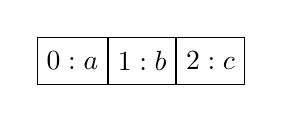
\begin{tikzpicture}
\matrix[nodes={draw,minimum size=6mm}] {
  \node {$0:a$}; & \node {$1:b$}; & \node {$2:c$};\\
};
\end{tikzpicture}

\noindent shows an array with three elements. The value of index 0 is $a$; the
value of index 1 is $b$; the value of index 2 is $c$.

\subsubsection{{\tt{}\protect\nwindexuse{DBUpdateEdgeSpeed}{DBUpdateEdgeSpeed}{NW15FRcE-3SpUqj-1}DBUpdateEdgeSpeed}(3)}
\label{sec:update-edge-speed}
The speed stored for each edge in the road network is the maximum free-flow
speed, in meters per second.  It can be updated with
{\tt{}\protect\nwindexuse{DBUpdateEdgeSpeed}{DBUpdateEdgeSpeed}{NW15FRcE-3SpUqj-1}DBUpdateEdgeSpeed}. The new speed {\tt{}nu} must be greater than or equal to 0,
otherwise constraint C9 will be violated. This method fails silently if
edge ({\tt{}v1}, {\tt{}v2}) does not exist.
\nwenddocs{}\nwbegincode{161}\sublabel{NW15FRcE-3SpUqj-1}\nwmargintag{{\nwtagstyle{}\subpageref{NW15FRcE-3SpUqj-1}}}\moddef{Update edge speed~{\nwtagstyle{}\subpageref{NW15FRcE-3SpUqj-1}}}\endmoddef\nwused{\\{NW15FRcE-4PbjF-2}}
public void DBUpdateEdgeSpeed(int v1, int v2, int nu) throws RuntimeException \{
  try \{
    PSClear(15, 131);
    PSAdd(15, nu, v1, v2);
    PSAdd(131, nu, v1, v2);
    PSSubmit(15, 131);
    conn.commit();
  \}
  \LA{}Catch and print \code{}SQLException\edoc{}~{\nwtagstyle{}\subpageref{NW15FRcE-4P0tKA-1}}\RA{}
\}
\nosublabel{NW15FRcE-3SpUqj-1-u1}\nwindexdefn{DBUpdateEdgeSpeed}{DBUpdateEdgeSpeed}{NW15FRcE-3SpUqj-1}\eatline
\nwidentdefs{\\{{DBUpdateEdgeSpeed}{DBUpdateEdgeSpeed}}}\nwidentuses{\\{{conn}{conn}}\\{{PSAdd}{PSAdd}}\\{{PSClear}{PSClear}}\\{{PSSubmit}{PSSubmit}}}\nwindexuse{conn}{conn}{NW15FRcE-3SpUqj-1}\nwindexuse{PSAdd}{PSAdd}{NW15FRcE-3SpUqj-1}\nwindexuse{PSClear}{PSClear}{NW15FRcE-3SpUqj-1}\nwindexuse{PSSubmit}{PSSubmit}{NW15FRcE-3SpUqj-1}\nwendcode{}\nwbegindocs{162}\nwdocspar
\subsubsection{{\tt{}\protect\nwindexuse{DBAddNewRequest}{DBAddNewRequest}{NW15FRcE-4ISWm4-1}DBAddNewRequest}(1)}
Array {\tt{}u} =

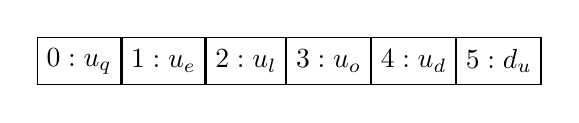
\begin{tikzpicture}
\matrix[nodes={draw,minimum size=6mm}] {
  \node {$0:u_q$}; & \node {$1:u_e$}; & \node {$2:u_l$};
 &\node {$3:u_o$}; & \node {$4:u_d$}; & \node {$5:d_u$};\\
};
\end{tikzpicture}

\noindent for user $u$. In order to use {\tt{}DBAddRequest}, $u_q$ must be
greater than 0, otherwise constraint C48 will be violated.

\nwenddocs{}\nwbegincode{163}\sublabel{NW15FRcE-4ISWm4-1}\nwmargintag{{\nwtagstyle{}\subpageref{NW15FRcE-4ISWm4-1}}}\moddef{Add new request~{\nwtagstyle{}\subpageref{NW15FRcE-4ISWm4-1}}}\endmoddef\nwused{\\{NW15FRcE-4PbjF-2}}
public int DBAddNewRequest(int[] u) throws RuntimeException \{
  try \{
    uid += 1;
    \LA{}..insert new user into user tables~{\nwtagstyle{}\subpageref{NW15FRcE-4ROa6q-1}}\RA{}
    \LA{}..insert new request into Table R~{\nwtagstyle{}\subpageref{NW15FRcE-2lKZoL-1}}\RA{}
    conn.commit();
    return uid;
  \}
  \LA{}Catch and print \code{}SQLException\edoc{}~{\nwtagstyle{}\subpageref{NW15FRcE-4P0tKA-1}}\RA{}
\}
\nosublabel{NW15FRcE-4ISWm4-1-u3}\nwindexdefn{DBAddNewRequest}{DBAddNewRequest}{NW15FRcE-4ISWm4-1}\eatline
\nwidentdefs{\\{{DBAddNewRequest}{DBAddNewRequest}}}\nwidentuses{\\{{conn}{conn}}\\{{uid}{uid}}}\nwindexuse{conn}{conn}{NW15FRcE-4ISWm4-1}\nwindexuse{uid}{uid}{NW15FRcE-4ISWm4-1}\nwendcode{}\nwbegincode{164}\sublabel{NW15FRcE-4ROa6q-1}\nwmargintag{{\nwtagstyle{}\subpageref{NW15FRcE-4ROa6q-1}}}\moddef{..insert new user into user tables~{\nwtagstyle{}\subpageref{NW15FRcE-4ROa6q-1}}}\endmoddef\nwused{\\{NW15FRcE-4ISWm4-1}\\{NW15FRcE-IYVQQ-1}}
PSClear(2, 3, 4, 5, 6, 7);
PSAdd(2, uid, u[0]);
PSAdd(3, uid, u[1]);
PSAdd(4, uid, u[2]);
PSAdd(5, uid, u[3]);
PSAdd(6, uid, u[4]);
PSAdd(7, uid, u[5]);
PSSubmit(2, 3, 4, 5, 6, 7);
\nwidentuses{\\{{PSAdd}{PSAdd}}\\{{PSClear}{PSClear}}\\{{PSSubmit}{PSSubmit}}\\{{uid}{uid}}}\nwindexuse{PSAdd}{PSAdd}{NW15FRcE-4ROa6q-1}\nwindexuse{PSClear}{PSClear}{NW15FRcE-4ROa6q-1}\nwindexuse{PSSubmit}{PSSubmit}{NW15FRcE-4ROa6q-1}\nwindexuse{uid}{uid}{NW15FRcE-4ROa6q-1}\nwendcode{}\nwbegindocs{165}\nwdocspar
\nwenddocs{}\nwbegincode{166}\sublabel{NW15FRcE-2lKZoL-1}\nwmargintag{{\nwtagstyle{}\subpageref{NW15FRcE-2lKZoL-1}}}\moddef{..insert new request into Table R~{\nwtagstyle{}\subpageref{NW15FRcE-2lKZoL-1}}}\endmoddef\nwused{\\{NW15FRcE-4ISWm4-1}}
PSClear(9);
PSAdd(9, uid, u[0], u[1], u[2], u[3], u[4], u[5]);
PSSubmit(9);
\nwidentuses{\\{{PSAdd}{PSAdd}}\\{{PSClear}{PSClear}}\\{{PSSubmit}{PSSubmit}}\\{{uid}{uid}}}\nwindexuse{PSAdd}{PSAdd}{NW15FRcE-2lKZoL-1}\nwindexuse{PSClear}{PSClear}{NW15FRcE-2lKZoL-1}\nwindexuse{PSSubmit}{PSSubmit}{NW15FRcE-2lKZoL-1}\nwindexuse{uid}{uid}{NW15FRcE-2lKZoL-1}\nwendcode{}\nwbegindocs{167}\nwdocspar
\subsubsection{{\tt{}\protect\nwindexuse{DBAddNewServer}{DBAddNewServer}{NW15FRcE-IYVQQ-1}DBAddNewServer}(2)}
Array {\tt{}u} =

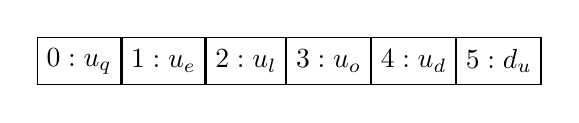
\begin{tikzpicture}
\matrix[nodes={draw,minimum size=6mm}] {
  \node {$0:u_q$}; & \node {$1:u_e$}; & \node {$2:u_l$};
 &\node {$3:u_o$}; & \node {$4:u_d$}; & \node {$5:d_u$};\\
};
\end{tikzpicture}

\noindent for user $u$. In order to use {\tt{}DBAddServer}, $u_q$ must be less
than 0, otherwise constraint C40 will be violated. Use {\tt{}route} to provide the
initial route. Array {\tt{}route} =

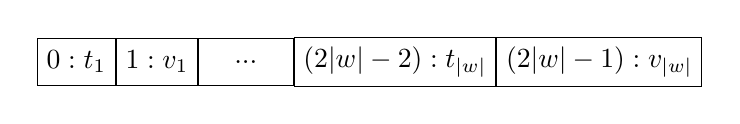
\begin{tikzpicture}
\matrix[nodes={draw,minimum size=6mm}] {
  \node {$0:t_1$}; & \node {$1:v_1$};
 &\node[minimum width=12mm] {...};
 &\node {$(2|w|-2):t_{|w|}$}; & \node {$(2|w|-1):v_{|w|}$};\\
};
\end{tikzpicture}

\noindent for route $w$.

\nwenddocs{}\nwbegincode{168}\sublabel{NW15FRcE-IYVQQ-1}\nwmargintag{{\nwtagstyle{}\subpageref{NW15FRcE-IYVQQ-1}}}\moddef{Add new server~{\nwtagstyle{}\subpageref{NW15FRcE-IYVQQ-1}}}\endmoddef\nwused{\\{NW15FRcE-4PbjF-2}}
public int DBAddNewServer(int[] u, int[] route) throws RuntimeException \{
  try \{
    int[] output = new int[] \{ \};
    int se = u[1];
    uid += 1;
    \LA{}..insert new user into user tables~{\nwtagstyle{}\subpageref{NW15FRcE-4ROa6q-1}}\RA{}
    \LA{}..insert new server into Table S~{\nwtagstyle{}\subpageref{NW15FRcE-1y8HBC-1}}\RA{}
    \LA{}..insert new server route into Table W~{\nwtagstyle{}\subpageref{NW15FRcE-2JTZnV-1}}\RA{}
    \LA{}..insert new server route into Table CW~{\nwtagstyle{}\subpageref{NW15FRcE-1H8Jm4-1}}\RA{}
    \LA{}..insert new server into Table CQ~{\nwtagstyle{}\subpageref{NW15FRcE-2ewFdp-1}}\RA{}
    conn.commit();
    return uid;
  \}
  \LA{}Catch and print \code{}SQLException\edoc{}~{\nwtagstyle{}\subpageref{NW15FRcE-4P0tKA-1}}\RA{}
\}
\nosublabel{NW15FRcE-IYVQQ-1-u6}\nwindexdefn{DBAddNewServer}{DBAddNewServer}{NW15FRcE-IYVQQ-1}\eatline
\nwidentdefs{\\{{DBAddNewServer}{DBAddNewServer}}}\nwidentuses{\\{{conn}{conn}}\\{{uid}{uid}}}\nwindexuse{conn}{conn}{NW15FRcE-IYVQQ-1}\nwindexuse{uid}{uid}{NW15FRcE-IYVQQ-1}\nwendcode{}\nwbegincode{169}\sublabel{NW15FRcE-1y8HBC-1}\nwmargintag{{\nwtagstyle{}\subpageref{NW15FRcE-1y8HBC-1}}}\moddef{..insert new server into Table S~{\nwtagstyle{}\subpageref{NW15FRcE-1y8HBC-1}}}\endmoddef\nwused{\\{NW15FRcE-IYVQQ-1}}
PSClear(8);
PSAdd(8, uid, u[0], u[1], u[2], u[3], u[4], u[5]);
PSSubmit(8);
\nwidentuses{\\{{PSAdd}{PSAdd}}\\{{PSClear}{PSClear}}\\{{PSSubmit}{PSSubmit}}\\{{uid}{uid}}}\nwindexuse{PSAdd}{PSAdd}{NW15FRcE-1y8HBC-1}\nwindexuse{PSClear}{PSClear}{NW15FRcE-1y8HBC-1}\nwindexuse{PSSubmit}{PSSubmit}{NW15FRcE-1y8HBC-1}\nwindexuse{uid}{uid}{NW15FRcE-1y8HBC-1}\nwendcode{}\nwbegindocs{170}\nwdocspar
\nwenddocs{}\nwbegincode{171}\sublabel{NW15FRcE-2JTZnV-1}\nwmargintag{{\nwtagstyle{}\subpageref{NW15FRcE-2JTZnV-1}}}\moddef{..insert new server route into Table W~{\nwtagstyle{}\subpageref{NW15FRcE-2JTZnV-1}}}\endmoddef\nwused{\\{NW15FRcE-IYVQQ-1}}
\LA{}Procedure to insert \code{}route\edoc{} into Table W~{\nwtagstyle{}\subpageref{NW15FRcE-1EP7t-1}}\RA{}
\nwendcode{}\nwbegindocs{172}\nwdocspar
The procedure to insert {\tt{}route} into Table W is written into its own chunk so
we can re-use it later. The first step is to add the first waypoint with
{\tt{}null} as its predecessor. Then we loop through the remaining waypoints.
\nwenddocs{}\nwbegincode{173}\sublabel{NW15FRcE-1EP7t-1}\nwmargintag{{\nwtagstyle{}\subpageref{NW15FRcE-1EP7t-1}}}\moddef{Procedure to insert \code{}route\edoc{} into Table W~{\nwtagstyle{}\subpageref{NW15FRcE-1EP7t-1}}}\endmoddef\nwused{\\{NW15FRcE-2JTZnV-1}\\{NW15FRcE-1cGW7n-1}}
PSClear(10);
PSAdd(10, uid, se, null, null, route[0], route[1], null, null);
for (int i = 0; i < (route.length - 3); i += 2) \{
  int t1 = route[i];
  int v1 = route[(i + 1)];
  int t2 = route[(i + 2)];
  int v2 = route[(i + 3)];
  output = DBFetch(46, 2, v1, v2);
  int dd = output[0];
  int nu = output[1];
  PSAdd(10, uid, se, t1, v1, t2, v2, dd, nu);
\}
PSSubmit(10);
\nwidentuses{\\{{DBFetch}{DBFetch}}\\{{PSAdd}{PSAdd}}\\{{PSClear}{PSClear}}\\{{PSSubmit}{PSSubmit}}\\{{uid}{uid}}}\nwindexuse{DBFetch}{DBFetch}{NW15FRcE-1EP7t-1}\nwindexuse{PSAdd}{PSAdd}{NW15FRcE-1EP7t-1}\nwindexuse{PSClear}{PSClear}{NW15FRcE-1EP7t-1}\nwindexuse{PSSubmit}{PSSubmit}{NW15FRcE-1EP7t-1}\nwindexuse{uid}{uid}{NW15FRcE-1EP7t-1}\nwendcode{}\nwbegindocs{174}\nwdocspar
\nwenddocs{}\nwbegincode{175}\sublabel{NW15FRcE-1H8Jm4-1}\nwmargintag{{\nwtagstyle{}\subpageref{NW15FRcE-1H8Jm4-1}}}\moddef{..insert new server route into Table CW~{\nwtagstyle{}\subpageref{NW15FRcE-1H8Jm4-1}}}\endmoddef\nwused{\\{NW15FRcE-IYVQQ-1}}
PSClear(11);
int te = route[(route.length - 2)];
PSAdd(11, uid, u[1], u[2], u[3], u[4], u[1], u[3], te, u[4]);
PSSubmit(11);
\nwidentuses{\\{{PSAdd}{PSAdd}}\\{{PSClear}{PSClear}}\\{{PSSubmit}{PSSubmit}}\\{{uid}{uid}}}\nwindexuse{PSAdd}{PSAdd}{NW15FRcE-1H8Jm4-1}\nwindexuse{PSClear}{PSClear}{NW15FRcE-1H8Jm4-1}\nwindexuse{PSSubmit}{PSSubmit}{NW15FRcE-1H8Jm4-1}\nwindexuse{uid}{uid}{NW15FRcE-1H8Jm4-1}\nwendcode{}\nwbegindocs{176}\nwdocspar
\nwenddocs{}\nwbegincode{177}\sublabel{NW15FRcE-2ewFdp-1}\nwmargintag{{\nwtagstyle{}\subpageref{NW15FRcE-2ewFdp-1}}}\moddef{..insert new server into Table CQ~{\nwtagstyle{}\subpageref{NW15FRcE-2ewFdp-1}}}\endmoddef\nwused{\\{NW15FRcE-IYVQQ-1}}
PSClear(14);
PSAdd(14, uid, u[0], u[1], null, u[1], u[3], null, u[0],
    null, null, null, null, null, 1);
PSSubmit(14);
\nwidentuses{\\{{PSAdd}{PSAdd}}\\{{PSClear}{PSClear}}\\{{PSSubmit}{PSSubmit}}\\{{uid}{uid}}}\nwindexuse{PSAdd}{PSAdd}{NW15FRcE-2ewFdp-1}\nwindexuse{PSClear}{PSClear}{NW15FRcE-2ewFdp-1}\nwindexuse{PSSubmit}{PSSubmit}{NW15FRcE-2ewFdp-1}\nwindexuse{uid}{uid}{NW15FRcE-2ewFdp-1}\nwendcode{}\nwbegindocs{178}\nwdocspar

\subsubsection{{\tt{}\protect\nwindexuse{DBUpdateServerRoute}{DBUpdateServerRoute}{NW15FRcE-4VFddh-1}DBUpdateServerRoute}(2)}
Array {\tt{}route} =

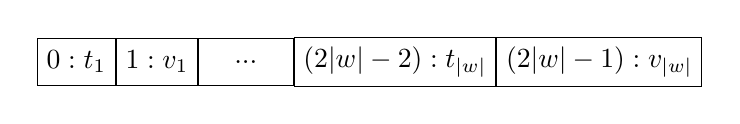
\begin{tikzpicture}
\matrix[nodes={draw,minimum size=6mm}] {
  \node {$0:t_1$}; & \node {$1:v_1$};
 &\node[minimum width=12mm] {...};
 &\node {$(2|w|-2):t_{|w|}$}; & \node {$(2|w|-1):v_{|w|}$};\\
};
\end{tikzpicture}

\noindent for route $w$.
\nwenddocs{}\nwbegincode{179}\sublabel{NW15FRcE-4VFddh-1}\nwmargintag{{\nwtagstyle{}\subpageref{NW15FRcE-4VFddh-1}}}\moddef{Update server route~{\nwtagstyle{}\subpageref{NW15FRcE-4VFddh-1}}}\endmoddef\nwused{\\{NW15FRcE-4PbjF-2}}
public void DBUpdateServerRoute(int sid, int[] route)
throws RuntimeException \{
  int[] output = new int[] \{ \};
  int se, sq;
  try \{
    \LA{}..fetch \code{}se\edoc{} and \code{}sq\edoc{}~{\nwtagstyle{}\subpageref{NW15FRcE-4HrAjg-1}}\RA{}
    \LA{}..update route~{\nwtagstyle{}\subpageref{NW15FRcE-4LV9nl-1}}\RA{}
    conn.commit();
  \}
  \LA{}Catch and print \code{}SQLException\edoc{}~{\nwtagstyle{}\subpageref{NW15FRcE-4P0tKA-1}}\RA{}
\}
\nosublabel{NW15FRcE-4VFddh-1-u3}\nwindexdefn{DBUpdateServerRoute}{DBUpdateServerRoute}{NW15FRcE-4VFddh-1}\eatline
\nwidentdefs{\\{{DBUpdateServerRoute}{DBUpdateServerRoute}}}\nwidentuses{\\{{conn}{conn}}}\nwindexuse{conn}{conn}{NW15FRcE-4VFddh-1}\nwendcode{}\nwbegincode{180}\sublabel{NW15FRcE-4HrAjg-1}\nwmargintag{{\nwtagstyle{}\subpageref{NW15FRcE-4HrAjg-1}}}\moddef{..fetch \code{}se\edoc{} and \code{}sq\edoc{}~{\nwtagstyle{}\subpageref{NW15FRcE-4HrAjg-1}}}\endmoddef\nwused{\\{NW15FRcE-4VFddh-1}\\{NW15FRcE-43w3hJ-1}\\{NW15FRcE-y828a-1}\\{NW15FRcE-lMiTm-1}}
output = DBFetch(48, 2, sid);
se = output[0];
sq = output[1];
\nwidentuses{\\{{DBFetch}{DBFetch}}}\nwindexuse{DBFetch}{DBFetch}{NW15FRcE-4HrAjg-1}\nwendcode{}\nwbegindocs{181}\nwdocspar
\nwenddocs{}\nwbegincode{182}\sublabel{NW15FRcE-4LV9nl-1}\nwmargintag{{\nwtagstyle{}\subpageref{NW15FRcE-4LV9nl-1}}}\moddef{..update route~{\nwtagstyle{}\subpageref{NW15FRcE-4LV9nl-1}}}\endmoddef\nwused{\\{NW15FRcE-4VFddh-1}\\{NW15FRcE-43w3hJ-1}\\{NW15FRcE-y828a-1}\\{NW15FRcE-lMiTm-1}}
\LA{}....delete remaining route~{\nwtagstyle{}\subpageref{NW15FRcE-4L1Zyt-1}}\RA{}
\LA{}....insert new remaining route~{\nwtagstyle{}\subpageref{NW15FRcE-1cGW7n-1}}\RA{}
\LA{}....update route endpoint~{\nwtagstyle{}\subpageref{NW15FRcE-vefz1-1}}\RA{}
\nwendcode{}\nwbegindocs{183}\nwdocspar
\nwenddocs{}\nwbegincode{184}\sublabel{NW15FRcE-4L1Zyt-1}\nwmargintag{{\nwtagstyle{}\subpageref{NW15FRcE-4L1Zyt-1}}}\moddef{....delete remaining route~{\nwtagstyle{}\subpageref{NW15FRcE-4L1Zyt-1}}}\endmoddef\nwused{\\{NW15FRcE-4LV9nl-1}}
PSClear(76);
PSAdd(76, sid, route[0]);
PSSubmit(76);
\nwidentuses{\\{{PSAdd}{PSAdd}}\\{{PSClear}{PSClear}}\\{{PSSubmit}{PSSubmit}}}\nwindexuse{PSAdd}{PSAdd}{NW15FRcE-4L1Zyt-1}\nwindexuse{PSClear}{PSClear}{NW15FRcE-4L1Zyt-1}\nwindexuse{PSSubmit}{PSSubmit}{NW15FRcE-4L1Zyt-1}\nwendcode{}\nwbegindocs{185}\nwdocspar
\nwenddocs{}\nwbegincode{186}\sublabel{NW15FRcE-1cGW7n-1}\nwmargintag{{\nwtagstyle{}\subpageref{NW15FRcE-1cGW7n-1}}}\moddef{....insert new remaining route~{\nwtagstyle{}\subpageref{NW15FRcE-1cGW7n-1}}}\endmoddef\nwused{\\{NW15FRcE-4LV9nl-1}}
\LA{}Procedure to insert \code{}route\edoc{} into Table W~{\nwtagstyle{}\subpageref{NW15FRcE-1EP7t-1}}\RA{}
\nwendcode{}\nwbegindocs{187}\nwdocspar
\nwenddocs{}\nwbegincode{188}\sublabel{NW15FRcE-vefz1-1}\nwmargintag{{\nwtagstyle{}\subpageref{NW15FRcE-vefz1-1}}}\moddef{....update route endpoint~{\nwtagstyle{}\subpageref{NW15FRcE-vefz1-1}}}\endmoddef\nwused{\\{NW15FRcE-4LV9nl-1}}
PSClear(77);
int te = route[(route.length - 2)];
int ve = route[(route.length - 1)];
PSAdd(77, te, ve, sid);
PSSubmit(77);
\nwidentuses{\\{{PSAdd}{PSAdd}}\\{{PSClear}{PSClear}}\\{{PSSubmit}{PSSubmit}}}\nwindexuse{PSAdd}{PSAdd}{NW15FRcE-vefz1-1}\nwindexuse{PSClear}{PSClear}{NW15FRcE-vefz1-1}\nwindexuse{PSSubmit}{PSSubmit}{NW15FRcE-vefz1-1}\nwendcode{}\nwbegindocs{189}\nwdocspar

\subsubsection{{\tt{}\protect\nwindexuse{DBUpdateServerSchedule}{DBUpdateServerSchedule}{NW15FRcE-43w3hJ-1}DBUpdateServerSchedule}(3)}
Array {\tt{}sched} =

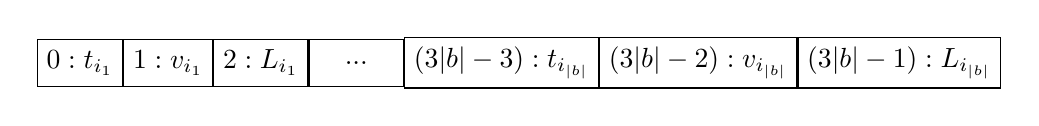
\begin{tikzpicture}
\matrix[nodes={draw,minimum size=6mm}] {
  \node {$0:t_{i_1}$}; & \node {$1:v_{i_1}$}; & \node {$2:L_{i_1}$};
 &\node[minimum width=12mm] {...};
 &\node {$(3|b|-3):t_{i_{|b|}}$};
 &\node {$(3|b|-2):v_{i_{|b|}}$};
 &\node {$(3|b|-1):L_{i_{|b|}}$}; \\
};
\end{tikzpicture}

\noindent for schedule $b$, where $(t_{i_j},v_{i_j})$ make up a waypoint and
$L_{i_j}$ is the label. Array {\tt{}route} =

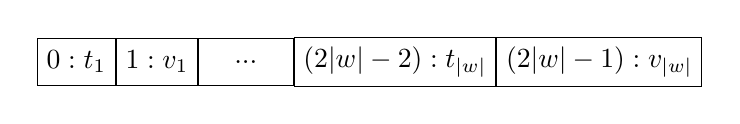
\begin{tikzpicture}
\matrix[nodes={draw,minimum size=6mm}] {
  \node {$0:t_1$}; & \node {$1:v_1$};
 &\node[minimum width=12mm] {...};
 &\node {$(2|w|-2):t_{|w|}$}; & \node {$(2|w|-1):v_{|w|}$};\\
};
\end{tikzpicture}

\noindent for route $w$.

Method {\tt{}\protect\nwindexuse{DBUpdateServerSchedule}{DBUpdateServerSchedule}{NW15FRcE-43w3hJ-1}DBUpdateServerSchedule} updates the \emph{remaining} route and
schedule.  No new stops should appear in the new schedule, otherwise foreign
key violations may occur. The point of the {\tt{}cache} is to store the
pick-up and drop-off times for each request in the schedule so that we
can use these values when we are inserting into Table CQ.
\nwenddocs{}\nwbegincode{190}\sublabel{NW15FRcE-43w3hJ-1}\nwmargintag{{\nwtagstyle{}\subpageref{NW15FRcE-43w3hJ-1}}}\moddef{Update server schedule~{\nwtagstyle{}\subpageref{NW15FRcE-43w3hJ-1}}}\endmoddef\nwused{\\{NW15FRcE-4PbjF-2}}
public void DBUpdateServerSchedule(int sid, int[] sched, int[] route)
throws RuntimeException \{
  int[] output = new int[] \{ \};
  int se, sq;
  Map<Integer, int[]> cache = new HashMap<>();
  try \{
    \LA{}..fetch \code{}se\edoc{} and \code{}sq\edoc{}~{\nwtagstyle{}\subpageref{NW15FRcE-4HrAjg-1}}\RA{}
    \LA{}..update route~{\nwtagstyle{}\subpageref{NW15FRcE-4LV9nl-1}}\RA{}
    \LA{}..update schedule~{\nwtagstyle{}\subpageref{NW15FRcE-2NqWTJ-1}}\RA{}
    conn.commit();
  \}
  \LA{}Catch and print \code{}SQLException\edoc{}~{\nwtagstyle{}\subpageref{NW15FRcE-4P0tKA-1}}\RA{}
\}
\nosublabel{NW15FRcE-43w3hJ-1-u4}\nwindexdefn{DBUpdateServerSchedule}{DBUpdateServerSchedule}{NW15FRcE-43w3hJ-1}\eatline
\nwidentdefs{\\{{DBUpdateServerSchedule}{DBUpdateServerSchedule}}}\nwidentuses{\\{{conn}{conn}}}\nwindexuse{conn}{conn}{NW15FRcE-43w3hJ-1}\nwendcode{}\nwbegindocs{191}Adding the {\tt{}-1} to the upper bound of {\tt{}j} skips over the last element
in the schedule, which is expected to be the server's destination.
\nwenddocs{}\nwbegincode{192}\sublabel{NW15FRcE-2NqWTJ-1}\nwmargintag{{\nwtagstyle{}\subpageref{NW15FRcE-2NqWTJ-1}}}\moddef{..update schedule~{\nwtagstyle{}\subpageref{NW15FRcE-2NqWTJ-1}}}\endmoddef\nwused{\\{NW15FRcE-43w3hJ-1}\\{NW15FRcE-lMiTm-1}}
int bound = ((sched.length/3) - 1);
\LA{}....update times in pd and cpd~{\nwtagstyle{}\subpageref{NW15FRcE-1cwA5Z-1}}\RA{}
\LA{}....populate the tp, td cache~{\nwtagstyle{}\subpageref{NW15FRcE-2G68mE-1}}\RA{}
\LA{}....insert into cq~{\nwtagstyle{}\subpageref{NW15FRcE-1eZXtL-1}}\RA{}
\nwendcode{}\nwbegindocs{193}\nwdocspar
\nwenddocs{}\nwbegincode{194}\sublabel{NW15FRcE-1cwA5Z-1}\nwmargintag{{\nwtagstyle{}\subpageref{NW15FRcE-1cwA5Z-1}}}\moddef{....update times in pd and cpd~{\nwtagstyle{}\subpageref{NW15FRcE-1cwA5Z-1}}}\endmoddef\nwused{\\{NW15FRcE-2NqWTJ-1}\\{NW15FRcE-2VQLMF-1}}
PSClear(82, 83, 84);
for (int j = 0; j < bound; j++) \{
  int tj = sched[(3*j)];
  int vj = sched[(3*j + 1)];
  int Lj = sched[(3*j + 2)];
  PSAdd(82, tj, vj, Lj);
  PSAdd(83, tj, vj, Lj);
  PSAdd(84, tj, vj, Lj);
\}
PSSubmit(82, 83, 84);
\nwidentuses{\\{{PSAdd}{PSAdd}}\\{{PSClear}{PSClear}}\\{{PSSubmit}{PSSubmit}}}\nwindexuse{PSAdd}{PSAdd}{NW15FRcE-1cwA5Z-1}\nwindexuse{PSClear}{PSClear}{NW15FRcE-1cwA5Z-1}\nwindexuse{PSSubmit}{PSSubmit}{NW15FRcE-1cwA5Z-1}\nwendcode{}\nwbegindocs{195}\nwdocspar
\nwenddocs{}\nwbegincode{196}\sublabel{NW15FRcE-2G68mE-1}\nwmargintag{{\nwtagstyle{}\subpageref{NW15FRcE-2G68mE-1}}}\moddef{....populate the tp, td cache~{\nwtagstyle{}\subpageref{NW15FRcE-2G68mE-1}}}\endmoddef\nwused{\\{NW15FRcE-2NqWTJ-1}}
for (int j = 0; j < bound; j++) \{
  int Lj = sched[(3*j + 2)];
  int rq, tp, td;
  if (!cache.containsKey(Lj)) \{
    rq = DBFetch(85, 1, Lj)[0];
    output = DBFetch(86, 2, Lj);
    tp = output[0];
    td = output[1];
    cache.put(Lj, new int[] \{ rq, tp, td \});
  \}
\}
\nwidentuses{\\{{DBFetch}{DBFetch}}}\nwindexuse{DBFetch}{DBFetch}{NW15FRcE-2G68mE-1}\nwendcode{}\nwbegindocs{197}\nwdocspar
\nwenddocs{}\nwbegincode{198}\sublabel{NW15FRcE-1eZXtL-1}\nwmargintag{{\nwtagstyle{}\subpageref{NW15FRcE-1eZXtL-1}}}\moddef{....insert into cq~{\nwtagstyle{}\subpageref{NW15FRcE-1eZXtL-1}}}\endmoddef\nwused{\\{NW15FRcE-2NqWTJ-1}\\{NW15FRcE-2VQLMF-1}}
PSClear(80);
PSAdd(80, sid, route[0]);
PSSubmit(80);
int t1, q1, o1;
output = DBFetch(87, 3, sched[0]);
t1 = output[0];
q1 = output[1];
o1 = output[2];
PSClear(14);
for (int j = 0; j < bound; j++) \{
  int t2 = sched[(3*j)];
  int v2 = sched[(3*j + 1)];
  int Lj = sched[(3*j + 2)];
  int[] qpd = cache.get(Lj);
  int q2 = (t2 == qpd[1] ? q1 + qpd[0] : q1 - qpd[0]);
  int o2 = o1 + 1;
  PSAdd(14, sid, sq, se, t1, t2, v2, q1, q2, Lj,
        qpd[0], qpd[1], qpd[2], o1, o2);
  t1 = t2;
  q1 = q2;
  o1 = o2;
\}
PSSubmit(14);
\nwidentuses{\\{{DBFetch}{DBFetch}}\\{{PSAdd}{PSAdd}}\\{{PSClear}{PSClear}}\\{{PSSubmit}{PSSubmit}}}\nwindexuse{DBFetch}{DBFetch}{NW15FRcE-1eZXtL-1}\nwindexuse{PSAdd}{PSAdd}{NW15FRcE-1eZXtL-1}\nwindexuse{PSClear}{PSClear}{NW15FRcE-1eZXtL-1}\nwindexuse{PSSubmit}{PSSubmit}{NW15FRcE-1eZXtL-1}\nwendcode{}\nwbegindocs{199}\nwdocspar

\subsubsection{{\tt{}\protect\nwindexuse{DBUpdateServerAddToSchedule}{DBUpdateServerAddToSchedule}{NW15FRcE-y828a-1}DBUpdateServerAddToSchedule}(4)}
A second cache, {\tt{}cache2}, is introduced to store the pick-up an drop-off
vertices so that we can use them when we insert into Table PD and CPD.
\nwenddocs{}\nwbegincode{200}\sublabel{NW15FRcE-y828a-1}\nwmargintag{{\nwtagstyle{}\subpageref{NW15FRcE-y828a-1}}}\moddef{Update server add to schedule~{\nwtagstyle{}\subpageref{NW15FRcE-y828a-1}}}\endmoddef\nwused{\\{NW15FRcE-4PbjF-2}}
public void DBUpdateServerAddToSchedule(
    int sid, int[] rid, int[] sched, int[] route)
throws RuntimeException \{
  int[] output = new int[] \{ \};
  int se, sq;
  Map<Integer, int[]> cache = new HashMap<>();
  Map<Integer, int[]> cache2 = new HashMap<>();
  try \{
    \LA{}..fetch \code{}se\edoc{} and \code{}sq\edoc{}~{\nwtagstyle{}\subpageref{NW15FRcE-4HrAjg-1}}\RA{}
    \LA{}..update route~{\nwtagstyle{}\subpageref{NW15FRcE-4LV9nl-1}}\RA{}
    \LA{}..update and add to schedule~{\nwtagstyle{}\subpageref{NW15FRcE-2VQLMF-1}}\RA{}
    conn.commit();
  \}
  \LA{}Catch and print \code{}SQLException\edoc{}~{\nwtagstyle{}\subpageref{NW15FRcE-4P0tKA-1}}\RA{}
\}
\nosublabel{NW15FRcE-y828a-1-u4}\nwindexdefn{DBUpdateServerAddToSchedule}{DBUpdateServerAddToSchedule}{NW15FRcE-y828a-1}\eatline
\nwidentdefs{\\{{DBUpdateServerAddToSchedule}{DBUpdateServerAddToSchedule}}}\nwidentuses{\\{{conn}{conn}}}\nwindexuse{conn}{conn}{NW15FRcE-y828a-1}\nwendcode{}\nwbegincode{201}\sublabel{NW15FRcE-2VQLMF-1}\nwmargintag{{\nwtagstyle{}\subpageref{NW15FRcE-2VQLMF-1}}}\moddef{..update and add to schedule~{\nwtagstyle{}\subpageref{NW15FRcE-2VQLMF-1}}}\endmoddef\nwused{\\{NW15FRcE-y828a-1}}
int bound = ((sched.length/3) - 1);
\LA{}....update times in pd and cpd~{\nwtagstyle{}\subpageref{NW15FRcE-1cwA5Z-1}}\RA{}
\LA{}....populate the tp, td cache and vp, vd cache~{\nwtagstyle{}\subpageref{NW15FRcE-10xBjT-1}}\RA{}
\LA{}....insert into cq~{\nwtagstyle{}\subpageref{NW15FRcE-1eZXtL-1}}\RA{}
\LA{}....insert into pd, cpd~{\nwtagstyle{}\subpageref{NW15FRcE-4fUZKI-1}}\RA{}
\nwendcode{}\nwbegindocs{202}\nwdocspar
\nwenddocs{}\nwbegincode{203}\sublabel{NW15FRcE-10xBjT-1}\nwmargintag{{\nwtagstyle{}\subpageref{NW15FRcE-10xBjT-1}}}\moddef{....populate the tp, td cache and vp, vd cache~{\nwtagstyle{}\subpageref{NW15FRcE-10xBjT-1}}}\endmoddef\nwused{\\{NW15FRcE-2VQLMF-1}}
for (int j = 0; j < bound; j++) \{
  int Lj = sched[(3*j + 2)];
  int rq, tp, vp;
  int td = -1;
  int vd = -1;
  if (!cache.containsKey(Lj)) \{
    rq = DBFetch(85, 1, Lj)[0];
    boolean flagged = false;
    \LA{}......check if new job~{\nwtagstyle{}\subpageref{NW15FRcE-2Hq38w-1}}\RA{}
    if (flagged) \{
      \LA{}......get tp, vp, td, vd of new job~{\nwtagstyle{}\subpageref{NW15FRcE-pddDf-1}}\RA{}
    \} else \{
      output = DBFetch(86, 2, Lj);
      tp = output[0];
      td = output[1];
    \}
    cache.put(Lj, new int[] \{ rq, tp, td \});
  \}
\}
\nwidentuses{\\{{DBFetch}{DBFetch}}}\nwindexuse{DBFetch}{DBFetch}{NW15FRcE-10xBjT-1}\nwendcode{}\nwbegindocs{204}\nwdocspar
\nwenddocs{}\nwbegincode{205}\sublabel{NW15FRcE-2Hq38w-1}\nwmargintag{{\nwtagstyle{}\subpageref{NW15FRcE-2Hq38w-1}}}\moddef{......check if new job~{\nwtagstyle{}\subpageref{NW15FRcE-2Hq38w-1}}}\endmoddef\nwused{\\{NW15FRcE-10xBjT-1}}
for (int r : rid) \{
  if (Lj == r) \{
    flagged = true;
    break;
  \}
\}
\nwendcode{}\nwbegindocs{206}\nwdocspar
\nwenddocs{}\nwbegincode{207}\sublabel{NW15FRcE-pddDf-1}\nwmargintag{{\nwtagstyle{}\subpageref{NW15FRcE-pddDf-1}}}\moddef{......get tp, vp, td, vd of new job~{\nwtagstyle{}\subpageref{NW15FRcE-pddDf-1}}}\endmoddef\nwused{\\{NW15FRcE-10xBjT-1}}
tp = sched[(3*j)];
vp = sched[(3*j + 1)];
for (int k = (j + 1); k < bound; k++) \{
  if (Lj == sched[(3*k + 2)]) \{
    td = sched[(3*k)];
    vd = sched[(3*k + 1)];
  \}
\}
cache2.put(Lj, new int[] \{ vp, vd \});
\nwendcode{}\nwbegindocs{208}\nwdocspar
\nwenddocs{}\nwbegincode{209}\sublabel{NW15FRcE-4fUZKI-1}\nwmargintag{{\nwtagstyle{}\subpageref{NW15FRcE-4fUZKI-1}}}\moddef{....insert into pd, cpd~{\nwtagstyle{}\subpageref{NW15FRcE-4fUZKI-1}}}\endmoddef\nwused{\\{NW15FRcE-2VQLMF-1}}
PSClear(12, 13);
int rq, re, rl, ro, rd;
int[] qpd, pd;
for (int r : rid) \{
  output = DBFetch(51, 5, r);
  rq = output[0];
  re = output[1];
  rl = output[2];
  ro = output[3];
  rd = output[4];
  qpd = cache.get(r);
  pd = cache2.get(r);
  PSAdd(12, sid, qpd[1], pd[0], r);
  PSAdd(12, sid, qpd[2], pd[1], r);
  PSAdd(13, sid, se, route[(route.length - 2)], qpd[1], pd[0], qpd[2], pd[1],
        r, rl, ro, rd);
\}
PSSubmit(12, 13);
\nwidentuses{\\{{DBFetch}{DBFetch}}\\{{PSAdd}{PSAdd}}\\{{PSClear}{PSClear}}\\{{PSSubmit}{PSSubmit}}}\nwindexuse{DBFetch}{DBFetch}{NW15FRcE-4fUZKI-1}\nwindexuse{PSAdd}{PSAdd}{NW15FRcE-4fUZKI-1}\nwindexuse{PSClear}{PSClear}{NW15FRcE-4fUZKI-1}\nwindexuse{PSSubmit}{PSSubmit}{NW15FRcE-4fUZKI-1}\nwendcode{}\nwbegindocs{210}\nwdocspar

\subsubsection{{\tt{}\protect\nwindexuse{DBUpdateServerRemoveFromSchedule}{DBUpdateServerRemoveFromSchedule}{NW15FRcE-lMiTm-1}DBUpdateServerRemoveFromSchedule}(4)}
\nwenddocs{}\nwbegincode{211}\sublabel{NW15FRcE-lMiTm-1}\nwmargintag{{\nwtagstyle{}\subpageref{NW15FRcE-lMiTm-1}}}\moddef{Update server remove from schedule~{\nwtagstyle{}\subpageref{NW15FRcE-lMiTm-1}}}\endmoddef\nwused{\\{NW15FRcE-4PbjF-2}}
public void DBUpdateServerRemoveFromSchedule(
    int sid, int[] rid, int[] sched, int[] route)
throws RuntimeException \{
  int[] output = new int[] \{ \};
  int se, sq;
  Map<Integer, int[]> cache = new HashMap<>();
  try \{
    \LA{}..fetch \code{}se\edoc{} and \code{}sq\edoc{}~{\nwtagstyle{}\subpageref{NW15FRcE-4HrAjg-1}}\RA{}
    \LA{}..update route~{\nwtagstyle{}\subpageref{NW15FRcE-4LV9nl-1}}\RA{}
    \LA{}..update schedule~{\nwtagstyle{}\subpageref{NW15FRcE-2NqWTJ-1}}\RA{}
    \LA{}..remove jobs from pd, cpd~{\nwtagstyle{}\subpageref{NW15FRcE-2PX0wC-1}}\RA{}
    conn.commit();
  \}
  \LA{}Catch and print \code{}SQLException\edoc{}~{\nwtagstyle{}\subpageref{NW15FRcE-4P0tKA-1}}\RA{}
\}
\nosublabel{NW15FRcE-lMiTm-1-u5}\nwindexdefn{DBUpdateServerRemoveFromSchedule}{DBUpdateServerRemoveFromSchedule}{NW15FRcE-lMiTm-1}\eatline
\nwidentdefs{\\{{DBUpdateServerRemoveFromSchedule}{DBUpdateServerRemoveFromSchedule}}}\nwidentuses{\\{{conn}{conn}}}\nwindexuse{conn}{conn}{NW15FRcE-lMiTm-1}\nwendcode{}\nwbegincode{212}\sublabel{NW15FRcE-2PX0wC-1}\nwmargintag{{\nwtagstyle{}\subpageref{NW15FRcE-2PX0wC-1}}}\moddef{..remove jobs from pd, cpd~{\nwtagstyle{}\subpageref{NW15FRcE-2PX0wC-1}}}\endmoddef\nwused{\\{NW15FRcE-lMiTm-1}}
PSClear(42, 43);
for (int r : rid) \{
  PSAdd(42, r);
  PSAdd(43, r);
\}
PSSubmit(42, 43);
\nwidentuses{\\{{PSAdd}{PSAdd}}\\{{PSClear}{PSClear}}\\{{PSSubmit}{PSSubmit}}}\nwindexuse{PSAdd}{PSAdd}{NW15FRcE-2PX0wC-1}\nwindexuse{PSClear}{PSClear}{NW15FRcE-2PX0wC-1}\nwindexuse{PSSubmit}{PSSubmit}{NW15FRcE-2PX0wC-1}\nwendcode{}\nwbegindocs{213}\nwdocspar

\subsection{Read Operations}
\label{sec:read-operations}
\subsubsection{{\tt{}DBQuery}(2)}
Run custom {\tt{}SELECT} queries against the database using
{\tt{}DBQuery}. The second parameter indicates the number of columns in the
{\tt{}SELECT} statement.
\nwenddocs{}\nwbegincode{214}\sublabel{NW15FRcE-2FtqIZ-1}\nwmargintag{{\nwtagstyle{}\subpageref{NW15FRcE-2FtqIZ-1}}}\moddef{Query custom statement~{\nwtagstyle{}\subpageref{NW15FRcE-2FtqIZ-1}}}\endmoddef\nwused{\\{NW15FRcE-4PbjF-3}}
public int[] DBQuery(String sql, int ncols) throws RuntimeException \{
  int[] output = new int[] \{ \};
  try \{
    Statement stmt = conn.createStatement(
      ResultSet.TYPE_SCROLL_INSENSITIVE, ResultSet.CONCUR_READ_ONLY);
    res = stmt.executeQuery(sql);
    if (res.last()) \{
      \LA{}..flatten results~{\nwtagstyle{}\subpageref{NW15FRcE-2Xu6MS-1}}\RA{}
    \}
  \}
  \LA{}Catch and print \code{}SQLException\edoc{}~{\nwtagstyle{}\subpageref{NW15FRcE-4P0tKA-1}}\RA{}
  return output;
\}
\nwidentuses{\\{{conn}{conn}}\\{{res}{res}}}\nwindexuse{conn}{conn}{NW15FRcE-2FtqIZ-1}\nwindexuse{res}{res}{NW15FRcE-2FtqIZ-1}\nwendcode{}\nwbegindocs{215}% def DBQuery

\subsubsection{{\tt{}\protect\nosublabel{NW15FRcE-2FtqIZ-1-u2}\protect\nwindexuse{DBQueryServer}{DBQueryServer}{NW15FRcE-3isdeu-1}DBQueryServer}(1)}
\nwenddocs{}\nwbegincode{216}\sublabel{NW15FRcE-3isdeu-1}\nwmargintag{{\nwtagstyle{}\subpageref{NW15FRcE-3isdeu-1}}}\moddef{Query ridesharing user~{\nwtagstyle{}\subpageref{NW15FRcE-3isdeu-1}}}\endmoddef\nwalsodefined{\\{NW15FRcE-3isdeu-2}}\nwused{\\{NW15FRcE-4PbjF-3}}
public int[] DBQueryServer(int sid) throws RuntimeException \{
  int[] output = new int[] \{ \};
  try \{
    output = DBFetch(70, 7, sid);
  \}
  \LA{}Catch and print \code{}SQLException\edoc{}~{\nwtagstyle{}\subpageref{NW15FRcE-4P0tKA-1}}\RA{}
  return output;
\}
\nosublabel{NW15FRcE-3isdeu-1-u1}\nwindexdefn{DBQueryServer}{DBQueryServer}{NW15FRcE-3isdeu-1}\eatline
\nwidentdefs{\\{{DBQueryServer}{DBQueryServer}}}\nwidentuses{\\{{DBFetch}{DBFetch}}}\nwindexuse{DBFetch}{DBFetch}{NW15FRcE-3isdeu-1}\nwendcode{}\nwbegindocs{217}\nwdocspar
\subsubsection{{\tt{}\protect\nwindexuse{DBQueryRequest}{DBQueryRequest}{NW15FRcE-3isdeu-2}DBQueryRequest}(1)}
\nwenddocs{}\nwbegincode{218}\sublabel{NW15FRcE-3isdeu-2}\nwmargintag{{\nwtagstyle{}\subpageref{NW15FRcE-3isdeu-2}}}\moddef{Query ridesharing user~{\nwtagstyle{}\subpageref{NW15FRcE-3isdeu-1}}}\plusendmoddef
public int[] DBQueryRequest(int rid) throws RuntimeException \{
  int[] output = new int[] \{ \};
  try \{
    output = DBFetch(75, 7, rid);
  \}
  \LA{}Catch and print \code{}SQLException\edoc{}~{\nwtagstyle{}\subpageref{NW15FRcE-4P0tKA-1}}\RA{}
  return output;
\}
\nosublabel{NW15FRcE-3isdeu-2-u1}\nwindexdefn{DBQueryRequest}{DBQueryRequest}{NW15FRcE-3isdeu-2}\eatline
\nwidentdefs{\\{{DBQueryRequest}{DBQueryRequest}}}\nwidentuses{\\{{DBFetch}{DBFetch}}}\nwindexuse{DBFetch}{DBFetch}{NW15FRcE-3isdeu-2}\nwendcode{}\nwbegindocs{219}\nwdocspar
\subsubsection{{\tt{}\protect\nwindexuse{DBQueryQueuedRequests}{DBQueryQueuedRequests}{NW15FRcE-3AGrxZ-1}DBQueryQueuedRequests}(1)}
\nwenddocs{}\nwbegincode{220}\sublabel{NW15FRcE-3AGrxZ-1}\nwmargintag{{\nwtagstyle{}\subpageref{NW15FRcE-3AGrxZ-1}}}\moddef{Query queued requests~{\nwtagstyle{}\subpageref{NW15FRcE-3AGrxZ-1}}}\endmoddef\nwused{\\{NW15FRcE-4PbjF-3}}
public int[] DBQueryQueuedRequests(int t) throws RuntimeException \{
  int[] output = new int[] \{ \};
  try \{
    output = DBFetch(68, 7, t, t);
  \}
  \LA{}Catch and print \code{}SQLException\edoc{}~{\nwtagstyle{}\subpageref{NW15FRcE-4P0tKA-1}}\RA{}
  return output;
\}
\nosublabel{NW15FRcE-3AGrxZ-1-u1}\nwindexdefn{DBQueryQueuedRequests}{DBQueryQueuedRequests}{NW15FRcE-3AGrxZ-1}\eatline
\nwidentdefs{\\{{DBQueryQueuedRequests}{DBQueryQueuedRequests}}}\nwidentuses{\\{{DBFetch}{DBFetch}}}\nwindexuse{DBFetch}{DBFetch}{NW15FRcE-3AGrxZ-1}\nwendcode{}\nwbegindocs{221}\nwdocspar
\subsubsection{{\tt{}\protect\nwindexuse{DBQueryServerLocationsAll}{DBQueryServerLocationsAll}{NW15FRcE-rvb17-1}DBQueryServerLocationsAll}(1)}
\nwenddocs{}\nwbegincode{222}\sublabel{NW15FRcE-rvb17-1}\nwmargintag{{\nwtagstyle{}\subpageref{NW15FRcE-rvb17-1}}}\moddef{Query all server locations~{\nwtagstyle{}\subpageref{NW15FRcE-rvb17-1}}}\endmoddef\nwused{\\{NW15FRcE-4PbjF-3}}
public int[] DBQueryServerLocationsAll(int t) throws RuntimeException \{
  int[] output = new int[] \{ \};
  try \{
    output = DBFetch(59, 3, t, t, t, t);
  \}
  \LA{}Catch and print \code{}SQLException\edoc{}~{\nwtagstyle{}\subpageref{NW15FRcE-4P0tKA-1}}\RA{}
  return output;
\}
\nosublabel{NW15FRcE-rvb17-1-u1}\nwindexdefn{DBQueryServerLocationsAll}{DBQueryServerLocationsAll}{NW15FRcE-rvb17-1}\eatline
\nwidentdefs{\\{{DBQueryServerLocationsAll}{DBQueryServerLocationsAll}}}\nwidentuses{\\{{DBFetch}{DBFetch}}}\nwindexuse{DBFetch}{DBFetch}{NW15FRcE-rvb17-1}\nwendcode{}\nwbegindocs{223}\nwdocspar
\subsubsection{{\tt{}\protect\nwindexuse{DBQueryServerLocationsActive}{DBQueryServerLocationsActive}{NW15FRcE-3UaQCb-1}DBQueryServerLocationsActive}(1)}
\nwenddocs{}\nwbegincode{224}\sublabel{NW15FRcE-3UaQCb-1}\nwmargintag{{\nwtagstyle{}\subpageref{NW15FRcE-3UaQCb-1}}}\moddef{Query active server locations~{\nwtagstyle{}\subpageref{NW15FRcE-3UaQCb-1}}}\endmoddef\nwused{\\{NW15FRcE-4PbjF-3}}
public int[] DBQueryServerLocationsActive(int t) throws RuntimeException \{
  int[] output = new int[] \{ \};
  try \{
    output = DBFetch(128, 3, t, t, t, t, t);
  \}
  \LA{}Catch and print \code{}SQLException\edoc{}~{\nwtagstyle{}\subpageref{NW15FRcE-4P0tKA-1}}\RA{}
  return output;
\}
\nosublabel{NW15FRcE-3UaQCb-1-u1}\nwindexdefn{DBQueryServerLocationsActive}{DBQueryServerLocationsActive}{NW15FRcE-3UaQCb-1}\eatline
\nwidentdefs{\\{{DBQueryServerLocationsActive}{DBQueryServerLocationsActive}}}\nwidentuses{\\{{DBFetch}{DBFetch}}}\nwindexuse{DBFetch}{DBFetch}{NW15FRcE-3UaQCb-1}\nwendcode{}\nwbegindocs{225}\nwdocspar
\subsubsection{{\tt{}\protect\nwindexuse{DBQueryRoute}{DBQueryRoute}{NW15FRcE-1AprqI-1}DBQueryRoute}(1)}
A vehicle's route can be retrieved if its corresponding {\tt{}sid} is known.
\nwenddocs{}\nwbegincode{226}\sublabel{NW15FRcE-1AprqI-1}\nwmargintag{{\nwtagstyle{}\subpageref{NW15FRcE-1AprqI-1}}}\moddef{Query routes~{\nwtagstyle{}\subpageref{NW15FRcE-1AprqI-1}}}\endmoddef\nwalsodefined{\\{NW15FRcE-1AprqI-2}}\nwused{\\{NW15FRcE-4PbjF-3}}
public int[] DBQueryRoute(int sid) throws RuntimeException \{
  int[] output = new int[] \{ \};
  try \{
    output = DBFetch(60, 2, sid);
  \}
  \LA{}Catch and print \code{}SQLException\edoc{}~{\nwtagstyle{}\subpageref{NW15FRcE-4P0tKA-1}}\RA{}
  return output;
\}
\nosublabel{NW15FRcE-1AprqI-1-u1}\nwindexdefn{DBQueryRoute}{DBQueryRoute}{NW15FRcE-1AprqI-1}\eatline
\nwidentdefs{\\{{DBQueryRoute}{DBQueryRoute}}}\nwidentuses{\\{{DBFetch}{DBFetch}}}\nwindexuse{DBFetch}{DBFetch}{NW15FRcE-1AprqI-1}\nwendcode{}\nwbegindocs{227}\nwdocspar
\subsubsection{{\tt{}\protect\nwindexuse{DBQueryRouteRemaining}{DBQueryRouteRemaining}{NW15FRcE-1AprqI-2}DBQueryRouteRemaining}(2)}
\nwenddocs{}\nwbegincode{228}\sublabel{NW15FRcE-1AprqI-2}\nwmargintag{{\nwtagstyle{}\subpageref{NW15FRcE-1AprqI-2}}}\moddef{Query routes~{\nwtagstyle{}\subpageref{NW15FRcE-1AprqI-1}}}\plusendmoddef
public int[] DBQueryRouteRemaining(int sid, int t) throws RuntimeException \{
  int[] output = new int[] \{ \};
  try \{
    output = DBFetch(129, 2, sid, t);
  \}
  \LA{}Catch and print \code{}SQLException\edoc{}~{\nwtagstyle{}\subpageref{NW15FRcE-4P0tKA-1}}\RA{}
  return output;
\}
\nosublabel{NW15FRcE-1AprqI-2-u1}\nwindexdefn{DBQueryRouteRemaining}{DBQueryRouteRemaining}{NW15FRcE-1AprqI-2}\eatline
\nwidentdefs{\\{{DBQueryRouteRemaining}{DBQueryRouteRemaining}}}\nwidentuses{\\{{DBFetch}{DBFetch}}}\nwindexuse{DBFetch}{DBFetch}{NW15FRcE-1AprqI-2}\nwendcode{}\nwbegindocs{229}\nwdocspar
\subsubsection{{\tt{}\protect\nwindexuse{DBQuerySchedule}{DBQuerySchedule}{NW15FRcE-3yA8FQ-1}DBQuerySchedule}(1)}
Similarly, a vehicle's schedule can be retrieved.
\footnote{Schedules may contain {\tt{}null} values in the labels. A null is recorded
as a 0 in the output array due to {\tt{}getInt} in {\tt{}\protect\nwindexuse{DBFetch}{DBFetch}{NW15FRcE-17Zt8W-1}DBFetch}.}
\nwenddocs{}\nwbegincode{230}\sublabel{NW15FRcE-3yA8FQ-1}\nwmargintag{{\nwtagstyle{}\subpageref{NW15FRcE-3yA8FQ-1}}}\moddef{Query schedules~{\nwtagstyle{}\subpageref{NW15FRcE-3yA8FQ-1}}}\endmoddef\nwalsodefined{\\{NW15FRcE-3yA8FQ-2}}\nwused{\\{NW15FRcE-4PbjF-3}}
public int[] DBQuerySchedule(int sid) throws RuntimeException \{
  int[] output = new int[] \{ \};
  try \{
    output = DBFetch(61, 4, sid);
  \}
  \LA{}Catch and print \code{}SQLException\edoc{}~{\nwtagstyle{}\subpageref{NW15FRcE-4P0tKA-1}}\RA{}
  return output;
\}
\nosublabel{NW15FRcE-3yA8FQ-1-u1}\nwindexdefn{DBQuerySchedule}{DBQuerySchedule}{NW15FRcE-3yA8FQ-1}\eatline
\nwidentdefs{\\{{DBQuerySchedule}{DBQuerySchedule}}}\nwidentuses{\\{{DBFetch}{DBFetch}}}\nwindexuse{DBFetch}{DBFetch}{NW15FRcE-3yA8FQ-1}\nwendcode{}\nwbegindocs{231}\nwdocspar
\subsubsection{{\tt{}\protect\nwindexuse{DBQueryScheduleRemaining}{DBQueryScheduleRemaining}{NW15FRcE-3yA8FQ-2}DBQueryScheduleRemaining}(2)}
\nwenddocs{}\nwbegincode{232}\sublabel{NW15FRcE-3yA8FQ-2}\nwmargintag{{\nwtagstyle{}\subpageref{NW15FRcE-3yA8FQ-2}}}\moddef{Query schedules~{\nwtagstyle{}\subpageref{NW15FRcE-3yA8FQ-1}}}\plusendmoddef
public int[] DBQueryScheduleRemaining(int sid, int t) throws RuntimeException \{
  int[] output = new int[] \{ \};
  try \{
    output = DBFetch(69, 4, sid, t);
  \}
  \LA{}Catch and print \code{}SQLException\edoc{}~{\nwtagstyle{}\subpageref{NW15FRcE-4P0tKA-1}}\RA{}
  return output;
\}
\nosublabel{NW15FRcE-3yA8FQ-2-u1}\nwindexdefn{DBQueryScheduleRemaining}{DBQueryScheduleRemaining}{NW15FRcE-3yA8FQ-2}\eatline
\nwidentdefs{\\{{DBQueryScheduleRemaining}{DBQueryScheduleRemaining}}}\nwidentuses{\\{{DBFetch}{DBFetch}}}\nwindexuse{DBFetch}{DBFetch}{NW15FRcE-3yA8FQ-2}\nwendcode{}\nwbegindocs{233}\nwdocspar
\subsubsection{{\tt{}\protect\nwindexuse{DBQueryCurrentLoad}{DBQueryCurrentLoad}{NW15FRcE-aKbeg-1}DBQueryCurrentLoad}(2)}
\nwenddocs{}\nwbegincode{234}\sublabel{NW15FRcE-aKbeg-1}\nwmargintag{{\nwtagstyle{}\subpageref{NW15FRcE-aKbeg-1}}}\moddef{Query current load~{\nwtagstyle{}\subpageref{NW15FRcE-aKbeg-1}}}\endmoddef\nwused{\\{NW15FRcE-4PbjF-3}}
public int[] DBQueryCurrentLoad(int sid, int t) throws RuntimeException \{
  int[] output = new int[] \{ \};
  try \{
    output = DBFetch(73, 1, sid, t);
  \}
  \LA{}Catch and print \code{}SQLException\edoc{}~{\nwtagstyle{}\subpageref{NW15FRcE-4P0tKA-1}}\RA{}
  return output;
\}
\nosublabel{NW15FRcE-aKbeg-1-u1}\nwindexdefn{DBQueryCurrentLoad}{DBQueryCurrentLoad}{NW15FRcE-aKbeg-1}\eatline
\nwidentdefs{\\{{DBQueryCurrentLoad}{DBQueryCurrentLoad}}}\nwidentuses{\\{{DBFetch}{DBFetch}}}\nwindexuse{DBFetch}{DBFetch}{NW15FRcE-aKbeg-1}\nwendcode{}\nwbegindocs{235}\nwdocspar
\subsubsection{{\tt{}\protect\nwindexuse{DBQueryCountVertices}{DBQueryCountVertices}{NW15FRcE-1Ang64-1}DBQueryCountVertices}(0)}
\nwenddocs{}\nwbegincode{236}\sublabel{NW15FRcE-1Ang64-1}\nwmargintag{{\nwtagstyle{}\subpageref{NW15FRcE-1Ang64-1}}}\moddef{Query various metrics~{\nwtagstyle{}\subpageref{NW15FRcE-1Ang64-1}}}\endmoddef\nwalsodefined{\\{NW15FRcE-1Ang64-2}\\{NW15FRcE-1Ang64-3}\\{NW15FRcE-1Ang64-4}\\{NW15FRcE-1Ang64-5}\\{NW15FRcE-1Ang64-6}\\{NW15FRcE-1Ang64-7}\\{NW15FRcE-1Ang64-8}\\{NW15FRcE-1Ang64-9}\\{NW15FRcE-1Ang64-A}\\{NW15FRcE-1Ang64-B}\\{NW15FRcE-1Ang64-C}\\{NW15FRcE-1Ang64-D}\\{NW15FRcE-1Ang64-E}\\{NW15FRcE-1Ang64-F}\\{NW15FRcE-1Ang64-G}\\{NW15FRcE-1Ang64-H}\\{NW15FRcE-1Ang64-I}\\{NW15FRcE-1Ang64-J}\\{NW15FRcE-1Ang64-K}\\{NW15FRcE-1Ang64-L}\\{NW15FRcE-1Ang64-M}\\{NW15FRcE-1Ang64-N}\\{NW15FRcE-1Ang64-O}\\{NW15FRcE-1Ang64-P}\\{NW15FRcE-1Ang64-Q}\\{NW15FRcE-1Ang64-R}\\{NW15FRcE-1Ang64-S}\\{NW15FRcE-1Ang64-T}\\{NW15FRcE-1Ang64-U}\\{NW15FRcE-1Ang64-V}\\{NW15FRcE-1Ang64-W}\\{NW15FRcE-1Ang64-X}\\{NW15FRcE-1Ang64-Y}\\{NW15FRcE-1Ang64-Z}\\{NW15FRcE-1Ang64-a}}\nwused{\\{NW15FRcE-4PbjF-3}}
public int[] DBQueryCountVertices() throws RuntimeException \{
  int[] output = new int[] \{ \};
  try \{
    output = DBFetch(62, 1);
  \}
  \LA{}Catch and print \code{}SQLException\edoc{}~{\nwtagstyle{}\subpageref{NW15FRcE-4P0tKA-1}}\RA{}
  return output;
\}
\nosublabel{NW15FRcE-1Ang64-1-u1}\nwindexdefn{DBQueryCountVertices}{DBQueryCountVertices}{NW15FRcE-1Ang64-1}\eatline
\nwidentdefs{\\{{DBQueryCountVertices}{DBQueryCountVertices}}}\nwidentuses{\\{{DBFetch}{DBFetch}}}\nwindexuse{DBFetch}{DBFetch}{NW15FRcE-1Ang64-1}\nwendcode{}\nwbegindocs{237}\nwdocspar
\subsubsection{{\tt{}\protect\nwindexuse{DBQueryCountEdges}{DBQueryCountEdges}{NW15FRcE-1Ang64-2}DBQueryCountEdges}(0)}
\nwenddocs{}\nwbegincode{238}\sublabel{NW15FRcE-1Ang64-2}\nwmargintag{{\nwtagstyle{}\subpageref{NW15FRcE-1Ang64-2}}}\moddef{Query various metrics~{\nwtagstyle{}\subpageref{NW15FRcE-1Ang64-1}}}\plusendmoddef
public int[] DBQueryCountEdges() throws RuntimeException \{
  int[] output = new int[] \{ \};
  try \{
    output = DBFetch(63, 1);
  \}
  \LA{}Catch and print \code{}SQLException\edoc{}~{\nwtagstyle{}\subpageref{NW15FRcE-4P0tKA-1}}\RA{}
  return output;
\}
\nosublabel{NW15FRcE-1Ang64-2-u1}\nwindexdefn{DBQueryCountEdges}{DBQueryCountEdges}{NW15FRcE-1Ang64-2}\eatline
\nwidentdefs{\\{{DBQueryCountEdges}{DBQueryCountEdges}}}\nwidentuses{\\{{DBFetch}{DBFetch}}}\nwindexuse{DBFetch}{DBFetch}{NW15FRcE-1Ang64-2}\nwendcode{}\nwbegindocs{239}\nwdocspar
\subsubsection{{\tt{}\protect\nwindexuse{DBQueryVertex}{DBQueryVertex}{NW15FRcE-1Ang64-3}DBQueryVertex}(1)}
Returned array =

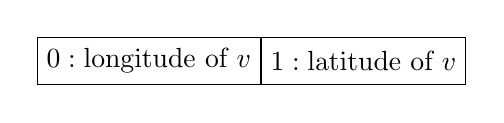
\begin{tikzpicture}
\matrix[nodes={draw,minimum size=6mm}] {
  \node {$0:\textrm{longitude of }v$};
& \node {$1:\textrm{latitude of }v$}; \\
};
\end{tikzpicture}

\noindent where parameter {\tt{}v} provides $v$.
\nwenddocs{}\nwbegincode{240}\sublabel{NW15FRcE-1Ang64-3}\nwmargintag{{\nwtagstyle{}\subpageref{NW15FRcE-1Ang64-3}}}\moddef{Query various metrics~{\nwtagstyle{}\subpageref{NW15FRcE-1Ang64-1}}}\plusendmoddef
public int[] DBQueryVertex(int v) throws RuntimeException \{
  int[] output = new int[] \{ \};
  try \{
    output = DBFetch(130, 2, v);
  \}
  \LA{}Catch and print \code{}SQLException\edoc{}~{\nwtagstyle{}\subpageref{NW15FRcE-4P0tKA-1}}\RA{}
  return output;
\}
\nosublabel{NW15FRcE-1Ang64-3-u1}\nwindexdefn{DBQueryVertex}{DBQueryVertex}{NW15FRcE-1Ang64-3}\eatline
\nwidentdefs{\\{{DBQueryVertex}{DBQueryVertex}}}\nwidentuses{\\{{DBFetch}{DBFetch}}}\nwindexuse{DBFetch}{DBFetch}{NW15FRcE-1Ang64-3}\nwendcode{}\nwbegindocs{241}\nwdocspar
\subsubsection{{\tt{}\protect\nwindexuse{DBQueryEdge}{DBQueryEdge}{NW15FRcE-1Ang64-4}DBQueryEdge}(2)}
Returned array =

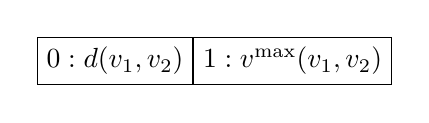
\begin{tikzpicture}
\matrix[nodes={draw,minimum size=6mm}] {
  \node {$0:d(v_1,v_2)$}; & \node {$1:v^\textrm{max}(v_1,v_2)$}; \\
};
\end{tikzpicture}

\noindent where parameter {\tt{}v1} provides $v_1$ and parameter
{\tt{}v2} provides $v_2$.
\nwenddocs{}\nwbegincode{242}\sublabel{NW15FRcE-1Ang64-4}\nwmargintag{{\nwtagstyle{}\subpageref{NW15FRcE-1Ang64-4}}}\moddef{Query various metrics~{\nwtagstyle{}\subpageref{NW15FRcE-1Ang64-1}}}\plusendmoddef
public int[] DBQueryEdge(int v1, int v2) throws RuntimeException \{
  int[] output = new int[] \{ \};
  try \{
    output = DBFetch(46, 2, v1, v2);
  \}
  \LA{}Catch and print \code{}SQLException\edoc{}~{\nwtagstyle{}\subpageref{NW15FRcE-4P0tKA-1}}\RA{}
  return output;
\}
\nosublabel{NW15FRcE-1Ang64-4-u1}\nwindexdefn{DBQueryEdge}{DBQueryEdge}{NW15FRcE-1Ang64-4}\eatline
\nwidentdefs{\\{{DBQueryEdge}{DBQueryEdge}}}\nwidentuses{\\{{DBFetch}{DBFetch}}}\nwindexuse{DBFetch}{DBFetch}{NW15FRcE-1Ang64-4}\nwendcode{}\nwbegindocs{243}\nwdocspar
\subsubsection{{\tt{}\protect\nwindexuse{DBQueryStatisticsEdges}{DBQueryStatisticsEdges}{NW15FRcE-1Ang64-5}DBQueryStatisticsEdges}(0)}
The following method returns six statistics: minimum edge weight,
maximum edge weight, average edge weight, minimum edge speed, maximum edge speed,
average edge speed.
\nwenddocs{}\nwbegincode{244}\sublabel{NW15FRcE-1Ang64-5}\nwmargintag{{\nwtagstyle{}\subpageref{NW15FRcE-1Ang64-5}}}\moddef{Query various metrics~{\nwtagstyle{}\subpageref{NW15FRcE-1Ang64-1}}}\plusendmoddef
public int[] DBQueryStatisticsEdges() throws RuntimeException \{
  int[] output = new int[] \{ \};
  try \{
    output = DBFetch(65, 6);
  \}
  \LA{}Catch and print \code{}SQLException\edoc{}~{\nwtagstyle{}\subpageref{NW15FRcE-4P0tKA-1}}\RA{}
  return output;
\}
\nosublabel{NW15FRcE-1Ang64-5-u1}\nwindexdefn{DBQueryStatisticsEdges}{DBQueryStatisticsEdges}{NW15FRcE-1Ang64-5}\eatline
\nwidentdefs{\\{{DBQueryStatisticsEdges}{DBQueryStatisticsEdges}}}\nwidentuses{\\{{DBFetch}{DBFetch}}}\nwindexuse{DBFetch}{DBFetch}{NW15FRcE-1Ang64-5}\nwendcode{}\nwbegindocs{245}\nwdocspar
\subsubsection{{\tt{}\protect\nwindexuse{DBQueryMBR}{DBQueryMBR}{NW15FRcE-1Ang64-6}DBQueryMBR}(0)}
The minimum bounding rectangle is
returned as four numbers: minimum longitude, maximum longitude, minimum
latitude, maximum latitude.
\nwenddocs{}\nwbegincode{246}\sublabel{NW15FRcE-1Ang64-6}\nwmargintag{{\nwtagstyle{}\subpageref{NW15FRcE-1Ang64-6}}}\moddef{Query various metrics~{\nwtagstyle{}\subpageref{NW15FRcE-1Ang64-1}}}\plusendmoddef
public int[] DBQueryMBR() throws RuntimeException \{
  int[] output = new int[] \{ \};
  try \{
    output = DBFetch(64, 4);
  \}
  \LA{}Catch and print \code{}SQLException\edoc{}~{\nwtagstyle{}\subpageref{NW15FRcE-4P0tKA-1}}\RA{}
  return output;
\}
\nosublabel{NW15FRcE-1Ang64-6-u1}\nwindexdefn{DBQueryMBR}{DBQueryMBR}{NW15FRcE-1Ang64-6}\eatline
\nwidentdefs{\\{{DBQueryMBR}{DBQueryMBR}}}\nwidentuses{\\{{DBFetch}{DBFetch}}}\nwindexuse{DBFetch}{DBFetch}{NW15FRcE-1Ang64-6}\nwendcode{}\nwbegindocs{247}\nwdocspar
\subsubsection{{\tt{}\protect\nwindexuse{DBQueryCountServers}{DBQueryCountServers}{NW15FRcE-1Ang64-7}DBQueryCountServers}(0)}
\nwenddocs{}\nwbegincode{248}\sublabel{NW15FRcE-1Ang64-7}\nwmargintag{{\nwtagstyle{}\subpageref{NW15FRcE-1Ang64-7}}}\moddef{Query various metrics~{\nwtagstyle{}\subpageref{NW15FRcE-1Ang64-1}}}\plusendmoddef
public int[] DBQueryCountServers() throws RuntimeException \{
  int[] output = new int[] \{ \};
  try \{
    output = DBFetch(66, 1);
  \}
  \LA{}Catch and print \code{}SQLException\edoc{}~{\nwtagstyle{}\subpageref{NW15FRcE-4P0tKA-1}}\RA{}
  return output;
\}
\nosublabel{NW15FRcE-1Ang64-7-u1}\nwindexdefn{DBQueryCountServers}{DBQueryCountServers}{NW15FRcE-1Ang64-7}\eatline
\nwidentdefs{\\{{DBQueryCountServers}{DBQueryCountServers}}}\nwidentuses{\\{{DBFetch}{DBFetch}}}\nwindexuse{DBFetch}{DBFetch}{NW15FRcE-1Ang64-7}\nwendcode{}\nwbegindocs{249}\nwdocspar
\subsubsection{{\tt{}\protect\nwindexuse{DBQueryCountRequests}{DBQueryCountRequests}{NW15FRcE-1Ang64-8}DBQueryCountRequests}(0)}
\nwenddocs{}\nwbegincode{250}\sublabel{NW15FRcE-1Ang64-8}\nwmargintag{{\nwtagstyle{}\subpageref{NW15FRcE-1Ang64-8}}}\moddef{Query various metrics~{\nwtagstyle{}\subpageref{NW15FRcE-1Ang64-1}}}\plusendmoddef
public int[] DBQueryCountRequests() throws RuntimeException \{
  int[] output = new int[] \{ \};
  try \{
    output = DBFetch(67, 1);
  \}
  \LA{}Catch and print \code{}SQLException\edoc{}~{\nwtagstyle{}\subpageref{NW15FRcE-4P0tKA-1}}\RA{}
  return output;
\}
\nosublabel{NW15FRcE-1Ang64-8-u1}\nwindexdefn{DBQueryCountRequests}{DBQueryCountRequests}{NW15FRcE-1Ang64-8}\eatline
\nwidentdefs{\\{{DBQueryCountRequests}{DBQueryCountRequests}}}\nwidentuses{\\{{DBFetch}{DBFetch}}}\nwindexuse{DBFetch}{DBFetch}{NW15FRcE-1Ang64-8}\nwendcode{}\nwbegindocs{251}\nwdocspar
\subsubsection{{\tt{}\protect\nwindexuse{DBQueryServerPendingAssignments}{DBQueryServerPendingAssignments}{NW15FRcE-1Ang64-9}DBQueryServerPendingAssignments}(2)}
\nwenddocs{}\nwbegincode{252}\sublabel{NW15FRcE-1Ang64-9}\nwmargintag{{\nwtagstyle{}\subpageref{NW15FRcE-1Ang64-9}}}\moddef{Query various metrics~{\nwtagstyle{}\subpageref{NW15FRcE-1Ang64-1}}}\plusendmoddef
public int[] DBQueryServerPendingAssignments(int sid, int t)
throws RuntimeException \{
  int[] output = new int[] \{ \};
  try \{
    output = DBFetch(100, 1, t, sid);
  \}
  \LA{}Catch and print \code{}SQLException\edoc{}~{\nwtagstyle{}\subpageref{NW15FRcE-4P0tKA-1}}\RA{}
  return output;
\}
\nosublabel{NW15FRcE-1Ang64-9-u1}\nwindexdefn{DBQueryServerPendingAssignments}{DBQueryServerPendingAssignments}{NW15FRcE-1Ang64-9}\eatline
\nwidentdefs{\\{{DBQueryServerPendingAssignments}{DBQueryServerPendingAssignments}}}\nwidentuses{\\{{DBFetch}{DBFetch}}}\nwindexuse{DBFetch}{DBFetch}{NW15FRcE-1Ang64-9}\nwendcode{}\nwbegindocs{253}\nwdocspar
\subsubsection{{\tt{}\protect\nwindexuse{DBQueryServerCompletedAssignments}{DBQueryServerCompletedAssignments}{NW15FRcE-1Ang64-A}DBQueryServerCompletedAssignments}(2)}
\nwenddocs{}\nwbegincode{254}\sublabel{NW15FRcE-1Ang64-A}\nwmargintag{{\nwtagstyle{}\subpageref{NW15FRcE-1Ang64-A}}}\moddef{Query various metrics~{\nwtagstyle{}\subpageref{NW15FRcE-1Ang64-1}}}\plusendmoddef
public int[] DBQueryServerCompletedAssignments(int sid, int t)
throws RuntimeException \{
  int[] output = new int[] \{ \};
  try \{
    output = DBFetch(101, 1, t, sid);
  \}
  \LA{}Catch and print \code{}SQLException\edoc{}~{\nwtagstyle{}\subpageref{NW15FRcE-4P0tKA-1}}\RA{}
  return output;
\}
\nosublabel{NW15FRcE-1Ang64-A-u1}\nwindexdefn{DBQueryServerCompletedAssignments}{DBQueryServerCompletedAssignments}{NW15FRcE-1Ang64-A}\eatline
\nwidentdefs{\\{{DBQueryServerCompletedAssignments}{DBQueryServerCompletedAssignments}}}\nwidentuses{\\{{DBFetch}{DBFetch}}}\nwindexuse{DBFetch}{DBFetch}{NW15FRcE-1Ang64-A}\nwendcode{}\nwbegindocs{255}\nwdocspar
\subsubsection{{\tt{}\protect\nwindexuse{DBQueryServiceRate}{DBQueryServiceRate}{NW15FRcE-1Ang64-B}DBQueryServiceRate}(0)}
\nwenddocs{}\nwbegincode{256}\sublabel{NW15FRcE-1Ang64-B}\nwmargintag{{\nwtagstyle{}\subpageref{NW15FRcE-1Ang64-B}}}\moddef{Query various metrics~{\nwtagstyle{}\subpageref{NW15FRcE-1Ang64-1}}}\plusendmoddef
public int[] DBQueryServiceRate() throws RuntimeException \{
  int[] output = new int[] \{ \};
  try \{
    output = DBFetch(102, 1);
  \}
  \LA{}Catch and print \code{}SQLException\edoc{}~{\nwtagstyle{}\subpageref{NW15FRcE-4P0tKA-1}}\RA{}
  return output;
\}
\nosublabel{NW15FRcE-1Ang64-B-u1}\nwindexdefn{DBQueryServiceRate}{DBQueryServiceRate}{NW15FRcE-1Ang64-B}\eatline
\nwidentdefs{\\{{DBQueryServiceRate}{DBQueryServiceRate}}}\nwidentuses{\\{{DBFetch}{DBFetch}}}\nwindexuse{DBFetch}{DBFetch}{NW15FRcE-1Ang64-B}\nwendcode{}\nwbegindocs{257}\nwdocspar
\subsubsection{{\tt{}\protect\nwindexuse{DBQueryBaseDistanceTotal}{DBQueryBaseDistanceTotal}{NW15FRcE-1Ang64-C}DBQueryBaseDistanceTotal}(0)}
\nwenddocs{}\nwbegincode{258}\sublabel{NW15FRcE-1Ang64-C}\nwmargintag{{\nwtagstyle{}\subpageref{NW15FRcE-1Ang64-C}}}\moddef{Query various metrics~{\nwtagstyle{}\subpageref{NW15FRcE-1Ang64-1}}}\plusendmoddef
public int[] DBQueryBaseDistanceTotal() throws RuntimeException \{
  int[] output = new int[] \{ \};
  try \{
    output = DBFetch(103, 1);
  \}
  \LA{}Catch and print \code{}SQLException\edoc{}~{\nwtagstyle{}\subpageref{NW15FRcE-4P0tKA-1}}\RA{}
  return output;
\}
\nosublabel{NW15FRcE-1Ang64-C-u1}\nwindexdefn{DBQueryBaseDistanceTotal}{DBQueryBaseDistanceTotal}{NW15FRcE-1Ang64-C}\eatline
\nwidentdefs{\\{{DBQueryBaseDistanceTotal}{DBQueryBaseDistanceTotal}}}\nwidentuses{\\{{DBFetch}{DBFetch}}}\nwindexuse{DBFetch}{DBFetch}{NW15FRcE-1Ang64-C}\nwendcode{}\nwbegindocs{259}\nwdocspar
\subsubsection{{\tt{}\protect\nwindexuse{DBQueryServerBaseDistanceTotal}{DBQueryServerBaseDistanceTotal}{NW15FRcE-1Ang64-D}DBQueryServerBaseDistanceTotal}(0)}
\nwenddocs{}\nwbegincode{260}\sublabel{NW15FRcE-1Ang64-D}\nwmargintag{{\nwtagstyle{}\subpageref{NW15FRcE-1Ang64-D}}}\moddef{Query various metrics~{\nwtagstyle{}\subpageref{NW15FRcE-1Ang64-1}}}\plusendmoddef
public int[] DBQueryServerBaseDistanceTotal() throws RuntimeException \{
  int[] output = new int[] \{ \};
  try \{
    output = DBFetch(110, 1);
  \}
  \LA{}Catch and print \code{}SQLException\edoc{}~{\nwtagstyle{}\subpageref{NW15FRcE-4P0tKA-1}}\RA{}
  return output;
\}
\nosublabel{NW15FRcE-1Ang64-D-u1}\nwindexdefn{DBQueryServerBaseDistanceTotal}{DBQueryServerBaseDistanceTotal}{NW15FRcE-1Ang64-D}\eatline
\nwidentdefs{\\{{DBQueryServerBaseDistanceTotal}{DBQueryServerBaseDistanceTotal}}}\nwidentuses{\\{{DBFetch}{DBFetch}}}\nwindexuse{DBFetch}{DBFetch}{NW15FRcE-1Ang64-D}\nwendcode{}\nwbegindocs{261}\nwdocspar
\subsubsection{{\tt{}\protect\nwindexuse{DBQueryRequestBaseDistanceTotal}{DBQueryRequestBaseDistanceTotal}{NW15FRcE-1Ang64-E}DBQueryRequestBaseDistanceTotal}(0)}
\nwenddocs{}\nwbegincode{262}\sublabel{NW15FRcE-1Ang64-E}\nwmargintag{{\nwtagstyle{}\subpageref{NW15FRcE-1Ang64-E}}}\moddef{Query various metrics~{\nwtagstyle{}\subpageref{NW15FRcE-1Ang64-1}}}\plusendmoddef
public int[] DBQueryRequestBaseDistanceTotal() throws RuntimeException \{
  int[] output = new int[] \{ \};
  try \{
    output = DBFetch(111, 1);
  \}
  \LA{}Catch and print \code{}SQLException\edoc{}~{\nwtagstyle{}\subpageref{NW15FRcE-4P0tKA-1}}\RA{}
  return output;
\}
\nosublabel{NW15FRcE-1Ang64-E-u1}\nwindexdefn{DBQueryRequestBaseDistanceTotal}{DBQueryRequestBaseDistanceTotal}{NW15FRcE-1Ang64-E}\eatline
\nwidentdefs{\\{{DBQueryRequestBaseDistanceTotal}{DBQueryRequestBaseDistanceTotal}}}\nwidentuses{\\{{DBFetch}{DBFetch}}}\nwindexuse{DBFetch}{DBFetch}{NW15FRcE-1Ang64-E}\nwendcode{}\nwbegindocs{263}\nwdocspar
\subsubsection{{\tt{}\protect\nwindexuse{DBQueryServerTravelDistance}{DBQueryServerTravelDistance}{NW15FRcE-1Ang64-F}DBQueryServerTravelDistance}(1)}
\nwenddocs{}\nwbegincode{264}\sublabel{NW15FRcE-1Ang64-F}\nwmargintag{{\nwtagstyle{}\subpageref{NW15FRcE-1Ang64-F}}}\moddef{Query various metrics~{\nwtagstyle{}\subpageref{NW15FRcE-1Ang64-1}}}\plusendmoddef
public int[] DBQueryServerTravelDistance(int sid) throws RuntimeException \{
  int[] output = new int[] \{ \};
  try \{
    output = DBFetch(104, 1, sid);
  \}
  \LA{}Catch and print \code{}SQLException\edoc{}~{\nwtagstyle{}\subpageref{NW15FRcE-4P0tKA-1}}\RA{}
  return output;
\}
\nosublabel{NW15FRcE-1Ang64-F-u1}\nwindexdefn{DBQueryServerTravelDistance}{DBQueryServerTravelDistance}{NW15FRcE-1Ang64-F}\eatline
\nwidentdefs{\\{{DBQueryServerTravelDistance}{DBQueryServerTravelDistance}}}\nwidentuses{\\{{DBFetch}{DBFetch}}}\nwindexuse{DBFetch}{DBFetch}{NW15FRcE-1Ang64-F}\nwendcode{}\nwbegindocs{265}\nwdocspar
\subsubsection{{\tt{}\protect\nwindexuse{DBQueryServerTravelDistanceTotal}{DBQueryServerTravelDistanceTotal}{NW15FRcE-1Ang64-G}DBQueryServerTravelDistanceTotal}(0)}
\nwenddocs{}\nwbegincode{266}\sublabel{NW15FRcE-1Ang64-G}\nwmargintag{{\nwtagstyle{}\subpageref{NW15FRcE-1Ang64-G}}}\moddef{Query various metrics~{\nwtagstyle{}\subpageref{NW15FRcE-1Ang64-1}}}\plusendmoddef
public int[] DBQueryServerTravelDistanceTotal() throws RuntimeException \{
  int[] output = new int[] \{ \};
  try \{
    output = DBFetch(105, 1);
  \}
  \LA{}Catch and print \code{}SQLException\edoc{}~{\nwtagstyle{}\subpageref{NW15FRcE-4P0tKA-1}}\RA{}
  return output;
\}
\nosublabel{NW15FRcE-1Ang64-G-u1}\nwindexdefn{DBQueryServerTravelDistanceTotal}{DBQueryServerTravelDistanceTotal}{NW15FRcE-1Ang64-G}\eatline
\nwidentdefs{\\{{DBQueryServerTravelDistanceTotal}{DBQueryServerTravelDistanceTotal}}}\nwidentuses{\\{{DBFetch}{DBFetch}}}\nwindexuse{DBFetch}{DBFetch}{NW15FRcE-1Ang64-G}\nwendcode{}\nwbegindocs{267}\nwdocspar
\subsubsection{{\tt{}\protect\nwindexuse{DBQueryServerCruisingDistance}{DBQueryServerCruisingDistance}{NW15FRcE-1Ang64-H}DBQueryServerCruisingDistance}(1)}
\nwenddocs{}\nwbegincode{268}\sublabel{NW15FRcE-1Ang64-H}\nwmargintag{{\nwtagstyle{}\subpageref{NW15FRcE-1Ang64-H}}}\moddef{Query various metrics~{\nwtagstyle{}\subpageref{NW15FRcE-1Ang64-1}}}\plusendmoddef
public int[] DBQueryServerCruisingDistance(int sid) throws RuntimeException \{
  int[] output = new int[] \{ \};
  try \{
    output = DBFetch(106, 1, sid);
  \}
  \LA{}Catch and print \code{}SQLException\edoc{}~{\nwtagstyle{}\subpageref{NW15FRcE-4P0tKA-1}}\RA{}
  return output;
\}
\nosublabel{NW15FRcE-1Ang64-H-u1}\nwindexdefn{DBQueryServerCruisingDistance}{DBQueryServerCruisingDistance}{NW15FRcE-1Ang64-H}\eatline
\nwidentdefs{\\{{DBQueryServerCruisingDistance}{DBQueryServerCruisingDistance}}}\nwidentuses{\\{{DBFetch}{DBFetch}}}\nwindexuse{DBFetch}{DBFetch}{NW15FRcE-1Ang64-H}\nwendcode{}\nwbegindocs{269}\nwdocspar
\subsubsection{{\tt{}\protect\nwindexuse{DBQueryServerCruisingDistanceTotal}{DBQueryServerCruisingDistanceTotal}{NW15FRcE-1Ang64-I}DBQueryServerCruisingDistanceTotal}(0)}
\nwenddocs{}\nwbegincode{270}\sublabel{NW15FRcE-1Ang64-I}\nwmargintag{{\nwtagstyle{}\subpageref{NW15FRcE-1Ang64-I}}}\moddef{Query various metrics~{\nwtagstyle{}\subpageref{NW15FRcE-1Ang64-1}}}\plusendmoddef
public int[] DBQueryServerCruisingDistanceTotal() throws RuntimeException \{
  int[] output = new int[] \{ \};
  try \{
    output = DBFetch(107, 1);
  \}
  \LA{}Catch and print \code{}SQLException\edoc{}~{\nwtagstyle{}\subpageref{NW15FRcE-4P0tKA-1}}\RA{}
  return output;
\}
\nosublabel{NW15FRcE-1Ang64-I-u1}\nwindexdefn{DBQueryServerCruisingDistanceTotal}{DBQueryServerCruisingDistanceTotal}{NW15FRcE-1Ang64-I}\eatline
\nwidentdefs{\\{{DBQueryServerCruisingDistanceTotal}{DBQueryServerCruisingDistanceTotal}}}\nwidentuses{\\{{DBFetch}{DBFetch}}}\nwindexuse{DBFetch}{DBFetch}{NW15FRcE-1Ang64-I}\nwendcode{}\nwbegindocs{271}\nwdocspar
\subsubsection{{\tt{}\protect\nwindexuse{DBQueryServerServiceDistance}{DBQueryServerServiceDistance}{NW15FRcE-1Ang64-J}DBQueryServerServiceDistance}(1)}
\nwenddocs{}\nwbegincode{272}\sublabel{NW15FRcE-1Ang64-J}\nwmargintag{{\nwtagstyle{}\subpageref{NW15FRcE-1Ang64-J}}}\moddef{Query various metrics~{\nwtagstyle{}\subpageref{NW15FRcE-1Ang64-1}}}\plusendmoddef
public int[] DBQueryServerServiceDistance(int sid) throws RuntimeException \{
  int[] output = new int[] \{ \};
  try \{
    output = DBFetch(108, 1, sid);
  \}
  \LA{}Catch and print \code{}SQLException\edoc{}~{\nwtagstyle{}\subpageref{NW15FRcE-4P0tKA-1}}\RA{}
  return output;
\}
\nosublabel{NW15FRcE-1Ang64-J-u1}\nwindexdefn{DBQueryServerServiceDistance}{DBQueryServerServiceDistance}{NW15FRcE-1Ang64-J}\eatline
\nwidentdefs{\\{{DBQueryServerServiceDistance}{DBQueryServerServiceDistance}}}\nwidentuses{\\{{DBFetch}{DBFetch}}}\nwindexuse{DBFetch}{DBFetch}{NW15FRcE-1Ang64-J}\nwendcode{}\nwbegindocs{273}\nwdocspar
\subsubsection{{\tt{}\protect\nwindexuse{DBQueryServerServiceDistanceTotal}{DBQueryServerServiceDistanceTotal}{NW15FRcE-1Ang64-K}DBQueryServerServiceDistanceTotal}(0)}
\nwenddocs{}\nwbegincode{274}\sublabel{NW15FRcE-1Ang64-K}\nwmargintag{{\nwtagstyle{}\subpageref{NW15FRcE-1Ang64-K}}}\moddef{Query various metrics~{\nwtagstyle{}\subpageref{NW15FRcE-1Ang64-1}}}\plusendmoddef
public int[] DBQueryServerServiceDistanceTotal() throws RuntimeException \{
  int[] output = new int[] \{ \};
  try \{
    output = DBFetch(109, 1);
  \}
  \LA{}Catch and print \code{}SQLException\edoc{}~{\nwtagstyle{}\subpageref{NW15FRcE-4P0tKA-1}}\RA{}
  return output;
\}
\nosublabel{NW15FRcE-1Ang64-K-u1}\nwindexdefn{DBQueryServerServiceDistanceTotal}{DBQueryServerServiceDistanceTotal}{NW15FRcE-1Ang64-K}\eatline
\nwidentdefs{\\{{DBQueryServerServiceDistanceTotal}{DBQueryServerServiceDistanceTotal}}}\nwidentuses{\\{{DBFetch}{DBFetch}}}\nwindexuse{DBFetch}{DBFetch}{NW15FRcE-1Ang64-K}\nwendcode{}\nwbegindocs{275}\nwdocspar
\subsubsection{{\tt{}\protect\nwindexuse{DBQueryRequestDetourDistance}{DBQueryRequestDetourDistance}{NW15FRcE-1Ang64-L}DBQueryRequestDetourDistance}(1)}
\nwenddocs{}\nwbegincode{276}\sublabel{NW15FRcE-1Ang64-L}\nwmargintag{{\nwtagstyle{}\subpageref{NW15FRcE-1Ang64-L}}}\moddef{Query various metrics~{\nwtagstyle{}\subpageref{NW15FRcE-1Ang64-1}}}\plusendmoddef
public int[] DBQueryRequestDetourDistance(int rid) throws RuntimeException \{
  int[] output = new int[] \{ \};
  try \{
    output = DBFetch(112, 1, rid);
  \}
  \LA{}Catch and print \code{}SQLException\edoc{}~{\nwtagstyle{}\subpageref{NW15FRcE-4P0tKA-1}}\RA{}
  return output;
\}
\nosublabel{NW15FRcE-1Ang64-L-u1}\nwindexdefn{DBQueryRequestDetourDistance}{DBQueryRequestDetourDistance}{NW15FRcE-1Ang64-L}\eatline
\nwidentdefs{\\{{DBQueryRequestDetourDistance}{DBQueryRequestDetourDistance}}}\nwidentuses{\\{{DBFetch}{DBFetch}}}\nwindexuse{DBFetch}{DBFetch}{NW15FRcE-1Ang64-L}\nwendcode{}\nwbegindocs{277}\nwdocspar
\subsubsection{{\tt{}\protect\nwindexuse{DBQueryRequestDetourDistanceTotal}{DBQueryRequestDetourDistanceTotal}{NW15FRcE-1Ang64-M}DBQueryRequestDetourDistanceTotal}(0)}
\nwenddocs{}\nwbegincode{278}\sublabel{NW15FRcE-1Ang64-M}\nwmargintag{{\nwtagstyle{}\subpageref{NW15FRcE-1Ang64-M}}}\moddef{Query various metrics~{\nwtagstyle{}\subpageref{NW15FRcE-1Ang64-1}}}\plusendmoddef
public int[] DBQueryRequestDetourDistanceTotal() throws RuntimeException \{
  int[] output = new int[] \{ \};
  try \{
    output = DBFetch(113, 1);
  \}
  \LA{}Catch and print \code{}SQLException\edoc{}~{\nwtagstyle{}\subpageref{NW15FRcE-4P0tKA-1}}\RA{}
  return output;
\}
\nosublabel{NW15FRcE-1Ang64-M-u1}\nwindexdefn{DBQueryRequestDetourDistanceTotal}{DBQueryRequestDetourDistanceTotal}{NW15FRcE-1Ang64-M}\eatline
\nwidentdefs{\\{{DBQueryRequestDetourDistanceTotal}{DBQueryRequestDetourDistanceTotal}}}\nwidentuses{\\{{DBFetch}{DBFetch}}}\nwindexuse{DBFetch}{DBFetch}{NW15FRcE-1Ang64-M}\nwendcode{}\nwbegindocs{279}\nwdocspar
\subsubsection{{\tt{}\protect\nwindexuse{DBQueryRequestTransitDistance}{DBQueryRequestTransitDistance}{NW15FRcE-1Ang64-N}DBQueryRequestTransitDistance}(1)}
\nwenddocs{}\nwbegincode{280}\sublabel{NW15FRcE-1Ang64-N}\nwmargintag{{\nwtagstyle{}\subpageref{NW15FRcE-1Ang64-N}}}\moddef{Query various metrics~{\nwtagstyle{}\subpageref{NW15FRcE-1Ang64-1}}}\plusendmoddef
public int[] DBQueryRequestTransitDistance(int rid) throws RuntimeException \{
  int[] output = new int[] \{ \};
  try \{
    output = DBFetch(114, 1, rid);
  \}
  \LA{}Catch and print \code{}SQLException\edoc{}~{\nwtagstyle{}\subpageref{NW15FRcE-4P0tKA-1}}\RA{}
  return output;
\}
\nosublabel{NW15FRcE-1Ang64-N-u1}\nwindexdefn{DBQueryRequestTransitDistance}{DBQueryRequestTransitDistance}{NW15FRcE-1Ang64-N}\eatline
\nwidentdefs{\\{{DBQueryRequestTransitDistance}{DBQueryRequestTransitDistance}}}\nwidentuses{\\{{DBFetch}{DBFetch}}}\nwindexuse{DBFetch}{DBFetch}{NW15FRcE-1Ang64-N}\nwendcode{}\nwbegindocs{281}\nwdocspar
\subsubsection{{\tt{}\protect\nwindexuse{DBQueryRequestTransitDistanceTotal}{DBQueryRequestTransitDistanceTotal}{NW15FRcE-1Ang64-O}DBQueryRequestTransitDistanceTotal}(0)}
\nwenddocs{}\nwbegincode{282}\sublabel{NW15FRcE-1Ang64-O}\nwmargintag{{\nwtagstyle{}\subpageref{NW15FRcE-1Ang64-O}}}\moddef{Query various metrics~{\nwtagstyle{}\subpageref{NW15FRcE-1Ang64-1}}}\plusendmoddef
public int[] DBQueryRequestTransitDistanceTotal() throws RuntimeException \{
  int[] output = new int[] \{ \};
  try \{
    output = DBFetch(115, 1);
  \}
  \LA{}Catch and print \code{}SQLException\edoc{}~{\nwtagstyle{}\subpageref{NW15FRcE-4P0tKA-1}}\RA{}
  return output;
\}
\nosublabel{NW15FRcE-1Ang64-O-u1}\nwindexdefn{DBQueryRequestTransitDistanceTotal}{DBQueryRequestTransitDistanceTotal}{NW15FRcE-1Ang64-O}\eatline
\nwidentdefs{\\{{DBQueryRequestTransitDistanceTotal}{DBQueryRequestTransitDistanceTotal}}}\nwidentuses{\\{{DBFetch}{DBFetch}}}\nwindexuse{DBFetch}{DBFetch}{NW15FRcE-1Ang64-O}\nwendcode{}\nwbegindocs{283}\nwdocspar
\subsubsection{{\tt{}\protect\nwindexuse{DBQueryServerTravelDuration}{DBQueryServerTravelDuration}{NW15FRcE-1Ang64-P}DBQueryServerTravelDuration}(1)}
\nwenddocs{}\nwbegincode{284}\sublabel{NW15FRcE-1Ang64-P}\nwmargintag{{\nwtagstyle{}\subpageref{NW15FRcE-1Ang64-P}}}\moddef{Query various metrics~{\nwtagstyle{}\subpageref{NW15FRcE-1Ang64-1}}}\plusendmoddef
public int[] DBQueryServerTravelDuration(int sid) throws RuntimeException \{
  int[] output = new int[] \{ \};
  try \{
    output = DBFetch(116, 1, sid);
  \}
  \LA{}Catch and print \code{}SQLException\edoc{}~{\nwtagstyle{}\subpageref{NW15FRcE-4P0tKA-1}}\RA{}
  return output;
\}
\nosublabel{NW15FRcE-1Ang64-P-u1}\nwindexdefn{DBQueryServerTravelDuration}{DBQueryServerTravelDuration}{NW15FRcE-1Ang64-P}\eatline
\nwidentdefs{\\{{DBQueryServerTravelDuration}{DBQueryServerTravelDuration}}}\nwidentuses{\\{{DBFetch}{DBFetch}}}\nwindexuse{DBFetch}{DBFetch}{NW15FRcE-1Ang64-P}\nwendcode{}\nwbegindocs{285}\nwdocspar
\subsubsection{{\tt{}\protect\nwindexuse{DBQueryServerTravelDurationTotal}{DBQueryServerTravelDurationTotal}{NW15FRcE-1Ang64-Q}DBQueryServerTravelDurationTotal}(0)}
\nwenddocs{}\nwbegincode{286}\sublabel{NW15FRcE-1Ang64-Q}\nwmargintag{{\nwtagstyle{}\subpageref{NW15FRcE-1Ang64-Q}}}\moddef{Query various metrics~{\nwtagstyle{}\subpageref{NW15FRcE-1Ang64-1}}}\plusendmoddef
public int[] DBQueryServerTravelDurationTotal() throws RuntimeException \{
  int[] output = new int[] \{ \};
  try \{
    output = DBFetch(117, 1);
  \}
  \LA{}Catch and print \code{}SQLException\edoc{}~{\nwtagstyle{}\subpageref{NW15FRcE-4P0tKA-1}}\RA{}
  return output;
\}
\nosublabel{NW15FRcE-1Ang64-Q-u1}\nwindexdefn{DBQueryServerTravelDurationTotal}{DBQueryServerTravelDurationTotal}{NW15FRcE-1Ang64-Q}\eatline
\nwidentdefs{\\{{DBQueryServerTravelDurationTotal}{DBQueryServerTravelDurationTotal}}}\nwidentuses{\\{{DBFetch}{DBFetch}}}\nwindexuse{DBFetch}{DBFetch}{NW15FRcE-1Ang64-Q}\nwendcode{}\nwbegindocs{287}\nwdocspar
\subsubsection{{\tt{}\protect\nwindexuse{DBQueryRequestPickupDuration}{DBQueryRequestPickupDuration}{NW15FRcE-1Ang64-R}DBQueryRequestPickupDuration}(1)}
\nwenddocs{}\nwbegincode{288}\sublabel{NW15FRcE-1Ang64-R}\nwmargintag{{\nwtagstyle{}\subpageref{NW15FRcE-1Ang64-R}}}\moddef{Query various metrics~{\nwtagstyle{}\subpageref{NW15FRcE-1Ang64-1}}}\plusendmoddef
public int[] DBQueryRequestPickupDuration(int rid) throws RuntimeException \{
  int[] output = new int[] \{ \};
  try \{
    output = DBFetch(118, 1, rid);
  \}
  \LA{}Catch and print \code{}SQLException\edoc{}~{\nwtagstyle{}\subpageref{NW15FRcE-4P0tKA-1}}\RA{}
  return output;
\}
\nosublabel{NW15FRcE-1Ang64-R-u1}\nwindexdefn{DBQueryRequestPickupDuration}{DBQueryRequestPickupDuration}{NW15FRcE-1Ang64-R}\eatline
\nwidentdefs{\\{{DBQueryRequestPickupDuration}{DBQueryRequestPickupDuration}}}\nwidentuses{\\{{DBFetch}{DBFetch}}}\nwindexuse{DBFetch}{DBFetch}{NW15FRcE-1Ang64-R}\nwendcode{}\nwbegindocs{289}\nwdocspar
\subsubsection{{\tt{}\protect\nwindexuse{DBQueryRequestPickupDurationTotal}{DBQueryRequestPickupDurationTotal}{NW15FRcE-1Ang64-S}DBQueryRequestPickupDurationTotal}(0)}
\nwenddocs{}\nwbegincode{290}\sublabel{NW15FRcE-1Ang64-S}\nwmargintag{{\nwtagstyle{}\subpageref{NW15FRcE-1Ang64-S}}}\moddef{Query various metrics~{\nwtagstyle{}\subpageref{NW15FRcE-1Ang64-1}}}\plusendmoddef
public int[] DBQueryRequestPickupDurationTotal() throws RuntimeException \{
  int[] output = new int[] \{ \};
  try \{
    output = DBFetch(119, 1);
  \}
  \LA{}Catch and print \code{}SQLException\edoc{}~{\nwtagstyle{}\subpageref{NW15FRcE-4P0tKA-1}}\RA{}
  return output;
\}
\nosublabel{NW15FRcE-1Ang64-S-u1}\nwindexdefn{DBQueryRequestPickupDurationTotal}{DBQueryRequestPickupDurationTotal}{NW15FRcE-1Ang64-S}\eatline
\nwidentdefs{\\{{DBQueryRequestPickupDurationTotal}{DBQueryRequestPickupDurationTotal}}}\nwidentuses{\\{{DBFetch}{DBFetch}}}\nwindexuse{DBFetch}{DBFetch}{NW15FRcE-1Ang64-S}\nwendcode{}\nwbegindocs{291}\nwdocspar
\subsubsection{{\tt{}\protect\nwindexuse{DBQueryRequestTransitDuration}{DBQueryRequestTransitDuration}{NW15FRcE-1Ang64-T}DBQueryRequestTransitDuration}(1)}
\nwenddocs{}\nwbegincode{292}\sublabel{NW15FRcE-1Ang64-T}\nwmargintag{{\nwtagstyle{}\subpageref{NW15FRcE-1Ang64-T}}}\moddef{Query various metrics~{\nwtagstyle{}\subpageref{NW15FRcE-1Ang64-1}}}\plusendmoddef
public int[] DBQueryRequestTransitDuration(int rid) throws RuntimeException \{
  int[] output = new int[] \{ \};
  try \{
    output = DBFetch(120, 1, rid);
  \}
  \LA{}Catch and print \code{}SQLException\edoc{}~{\nwtagstyle{}\subpageref{NW15FRcE-4P0tKA-1}}\RA{}
  return output;
\}
\nosublabel{NW15FRcE-1Ang64-T-u1}\nwindexdefn{DBQueryRequestTransitDuration}{DBQueryRequestTransitDuration}{NW15FRcE-1Ang64-T}\eatline
\nwidentdefs{\\{{DBQueryRequestTransitDuration}{DBQueryRequestTransitDuration}}}\nwidentuses{\\{{DBFetch}{DBFetch}}}\nwindexuse{DBFetch}{DBFetch}{NW15FRcE-1Ang64-T}\nwendcode{}\nwbegindocs{293}\nwdocspar
\subsubsection{{\tt{}\protect\nwindexuse{DBQueryRequestTransitDurationTotal}{DBQueryRequestTransitDurationTotal}{NW15FRcE-1Ang64-U}DBQueryRequestTransitDurationTotal}(0)}
\nwenddocs{}\nwbegincode{294}\sublabel{NW15FRcE-1Ang64-U}\nwmargintag{{\nwtagstyle{}\subpageref{NW15FRcE-1Ang64-U}}}\moddef{Query various metrics~{\nwtagstyle{}\subpageref{NW15FRcE-1Ang64-1}}}\plusendmoddef
public int[] DBQueryRequestTransitDurationTotal() throws RuntimeException \{
  int[] output = new int[] \{ \};
  try \{
    output = DBFetch(121, 1);
  \}
  \LA{}Catch and print \code{}SQLException\edoc{}~{\nwtagstyle{}\subpageref{NW15FRcE-4P0tKA-1}}\RA{}
  return output;
\}
\nosublabel{NW15FRcE-1Ang64-U-u1}\nwindexdefn{DBQueryRequestTransitDurationTotal}{DBQueryRequestTransitDurationTotal}{NW15FRcE-1Ang64-U}\eatline
\nwidentdefs{\\{{DBQueryRequestTransitDurationTotal}{DBQueryRequestTransitDurationTotal}}}\nwidentuses{\\{{DBFetch}{DBFetch}}}\nwindexuse{DBFetch}{DBFetch}{NW15FRcE-1Ang64-U}\nwendcode{}\nwbegindocs{295}\nwdocspar
\subsubsection{{\tt{}\protect\nwindexuse{DBQueryRequestTravelDuration}{DBQueryRequestTravelDuration}{NW15FRcE-1Ang64-V}DBQueryRequestTravelDuration}(1)}
\nwenddocs{}\nwbegincode{296}\sublabel{NW15FRcE-1Ang64-V}\nwmargintag{{\nwtagstyle{}\subpageref{NW15FRcE-1Ang64-V}}}\moddef{Query various metrics~{\nwtagstyle{}\subpageref{NW15FRcE-1Ang64-1}}}\plusendmoddef
public int[] DBQueryRequestTravelDuration(int rid) throws RuntimeException \{
  int[] output = new int[] \{ \};
  try \{
    output = DBFetch(122, 1, rid);
  \}
  \LA{}Catch and print \code{}SQLException\edoc{}~{\nwtagstyle{}\subpageref{NW15FRcE-4P0tKA-1}}\RA{}
  return output;
\}
\nosublabel{NW15FRcE-1Ang64-V-u1}\nwindexdefn{DBQueryRequestTravelDuration}{DBQueryRequestTravelDuration}{NW15FRcE-1Ang64-V}\eatline
\nwidentdefs{\\{{DBQueryRequestTravelDuration}{DBQueryRequestTravelDuration}}}\nwidentuses{\\{{DBFetch}{DBFetch}}}\nwindexuse{DBFetch}{DBFetch}{NW15FRcE-1Ang64-V}\nwendcode{}\nwbegindocs{297}\nwdocspar
\subsubsection{{\tt{}\protect\nwindexuse{DBQueryRequestTravelDurationTotal}{DBQueryRequestTravelDurationTotal}{NW15FRcE-1Ang64-W}DBQueryRequestTravelDurationTotal}(0)}
\nwenddocs{}\nwbegincode{298}\sublabel{NW15FRcE-1Ang64-W}\nwmargintag{{\nwtagstyle{}\subpageref{NW15FRcE-1Ang64-W}}}\moddef{Query various metrics~{\nwtagstyle{}\subpageref{NW15FRcE-1Ang64-1}}}\plusendmoddef
public int[] DBQueryRequestTravelDurationTotal() throws RuntimeException \{
  int[] output = new int[] \{ \};
  try \{
    output = DBFetch(123, 1);
  \}
  \LA{}Catch and print \code{}SQLException\edoc{}~{\nwtagstyle{}\subpageref{NW15FRcE-4P0tKA-1}}\RA{}
  return output;
\}
\nosublabel{NW15FRcE-1Ang64-W-u1}\nwindexdefn{DBQueryRequestTravelDurationTotal}{DBQueryRequestTravelDurationTotal}{NW15FRcE-1Ang64-W}\eatline
\nwidentdefs{\\{{DBQueryRequestTravelDurationTotal}{DBQueryRequestTravelDurationTotal}}}\nwidentuses{\\{{DBFetch}{DBFetch}}}\nwindexuse{DBFetch}{DBFetch}{NW15FRcE-1Ang64-W}\nwendcode{}\nwbegindocs{299}\nwdocspar
\subsubsection{{\tt{}\protect\nwindexuse{DBQueryRequestDepartureTime}{DBQueryRequestDepartureTime}{NW15FRcE-1Ang64-X}DBQueryRequestDepartureTime}(1)}
\nwenddocs{}\nwbegincode{300}\sublabel{NW15FRcE-1Ang64-X}\nwmargintag{{\nwtagstyle{}\subpageref{NW15FRcE-1Ang64-X}}}\moddef{Query various metrics~{\nwtagstyle{}\subpageref{NW15FRcE-1Ang64-1}}}\plusendmoddef
public int[] DBQueryRequestDepartureTime(int rid) throws RuntimeException \{
  int[] output = new int[] \{ \};
  try \{
    output = DBFetch(124, 1, rid);
  \}
  \LA{}Catch and print \code{}SQLException\edoc{}~{\nwtagstyle{}\subpageref{NW15FRcE-4P0tKA-1}}\RA{}
  return output;
\}
\nosublabel{NW15FRcE-1Ang64-X-u1}\nwindexdefn{DBQueryRequestDepartureTime}{DBQueryRequestDepartureTime}{NW15FRcE-1Ang64-X}\eatline
\nwidentdefs{\\{{DBQueryRequestDepartureTime}{DBQueryRequestDepartureTime}}}\nwidentuses{\\{{DBFetch}{DBFetch}}}\nwindexuse{DBFetch}{DBFetch}{NW15FRcE-1Ang64-X}\nwendcode{}\nwbegindocs{301}\nwdocspar
\subsubsection{{\tt{}\protect\nwindexuse{DBQueryServerDepartureTime}{DBQueryServerDepartureTime}{NW15FRcE-1Ang64-Y}DBQueryServerDepartureTime}(1)}
\nwenddocs{}\nwbegincode{302}\sublabel{NW15FRcE-1Ang64-Y}\nwmargintag{{\nwtagstyle{}\subpageref{NW15FRcE-1Ang64-Y}}}\moddef{Query various metrics~{\nwtagstyle{}\subpageref{NW15FRcE-1Ang64-1}}}\plusendmoddef
public int[] DBQueryServerDepartureTime(int sid) throws RuntimeException \{
  int[] output = new int[] \{ \};
  try \{
    output = DBFetch(125, 1, sid);
  \}
  \LA{}Catch and print \code{}SQLException\edoc{}~{\nwtagstyle{}\subpageref{NW15FRcE-4P0tKA-1}}\RA{}
  return output;
\}
\nosublabel{NW15FRcE-1Ang64-Y-u1}\nwindexdefn{DBQueryServerDepartureTime}{DBQueryServerDepartureTime}{NW15FRcE-1Ang64-Y}\eatline
\nwidentdefs{\\{{DBQueryServerDepartureTime}{DBQueryServerDepartureTime}}}\nwidentuses{\\{{DBFetch}{DBFetch}}}\nwindexuse{DBFetch}{DBFetch}{NW15FRcE-1Ang64-Y}\nwendcode{}\nwbegindocs{303}\nwdocspar
\subsubsection{{\tt{}\protect\nwindexuse{DBQueryRequestArrivalTime}{DBQueryRequestArrivalTime}{NW15FRcE-1Ang64-Z}DBQueryRequestArrivalTime}(1)}
\nwenddocs{}\nwbegincode{304}\sublabel{NW15FRcE-1Ang64-Z}\nwmargintag{{\nwtagstyle{}\subpageref{NW15FRcE-1Ang64-Z}}}\moddef{Query various metrics~{\nwtagstyle{}\subpageref{NW15FRcE-1Ang64-1}}}\plusendmoddef
public int[] DBQueryRequestArrivalTime(int rid) throws RuntimeException \{
  int[] output = new int[] \{ \};
  try \{
    output = DBFetch(126, 1, rid);
  \}
  \LA{}Catch and print \code{}SQLException\edoc{}~{\nwtagstyle{}\subpageref{NW15FRcE-4P0tKA-1}}\RA{}
  return output;
\}
\nosublabel{NW15FRcE-1Ang64-Z-u1}\nwindexdefn{DBQueryRequestArrivalTime}{DBQueryRequestArrivalTime}{NW15FRcE-1Ang64-Z}\eatline
\nwidentdefs{\\{{DBQueryRequestArrivalTime}{DBQueryRequestArrivalTime}}}\nwidentuses{\\{{DBFetch}{DBFetch}}}\nwindexuse{DBFetch}{DBFetch}{NW15FRcE-1Ang64-Z}\nwendcode{}\nwbegindocs{305}\nwdocspar
\subsubsection{{\tt{}\protect\nwindexuse{DBQueryServerArrivalTime}{DBQueryServerArrivalTime}{NW15FRcE-1Ang64-a}DBQueryServerArrivalTime}(1)}
\nwenddocs{}\nwbegincode{306}\sublabel{NW15FRcE-1Ang64-a}\nwmargintag{{\nwtagstyle{}\subpageref{NW15FRcE-1Ang64-a}}}\moddef{Query various metrics~{\nwtagstyle{}\subpageref{NW15FRcE-1Ang64-1}}}\plusendmoddef
public int[] DBQueryServerArrivalTime(int sid) throws RuntimeException \{
  int[] output = new int[] \{ \};
  try \{
    output = DBFetch(127, 1, sid);
  \}
  \LA{}Catch and print \code{}SQLException\edoc{}~{\nwtagstyle{}\subpageref{NW15FRcE-4P0tKA-1}}\RA{}
  return output;
\}
\nosublabel{NW15FRcE-1Ang64-a-u1}\nwindexdefn{DBQueryServerArrivalTime}{DBQueryServerArrivalTime}{NW15FRcE-1Ang64-a}\eatline
\nwidentdefs{\\{{DBQueryServerArrivalTime}{DBQueryServerArrivalTime}}}\nwidentuses{\\{{DBFetch}{DBFetch}}}\nwindexuse{DBFetch}{DBFetch}{NW15FRcE-1Ang64-a}\nwendcode{}\nwbegindocs{307}\nwdocspar
\section{Private Methods}
\label{sec:private}
\nwenddocs{}\nwbegincode{308}\sublabel{NW15FRcE-XGFF1-1}\nwmargintag{{\nwtagstyle{}\subpageref{NW15FRcE-XGFF1-1}}}\moddef{\code{}Storage\edoc{} private methods~{\nwtagstyle{}\subpageref{NW15FRcE-XGFF1-1}}}\endmoddef\nwused{\\{NW15FRcE-3TAldU-1}}
  \LA{}Print a message~{\nwtagstyle{}\subpageref{NW15FRcE-2wEn3G-1}}\RA{}
  \LA{}Prepare a prepared statement~{\nwtagstyle{}\subpageref{NW15FRcE-4UQpM2-1}}\RA{}
  \LA{}Fetch items from database~{\nwtagstyle{}\subpageref{NW15FRcE-17Zt8W-1}}\RA{}
  \LA{}Fill prepared statement~{\nwtagstyle{}\subpageref{NW15FRcE-1ZE0ye-1}}\RA{}
  \LA{}Clear prepared statement batch~{\nwtagstyle{}\subpageref{NW15FRcE-I2riE-1}}\RA{}
  \LA{}Submit prepared statement batch~{\nwtagstyle{}\subpageref{NW15FRcE-322zJf-1}}\RA{}
  \LA{}Initialize statements~{\nwtagstyle{}\subpageref{NW15FRcE-1g2xnv-1}}\RA{}
\nwendcode{}\nwbegindocs{309}\nwdocspar
\subsection{{\tt{}\protect\nosublabel{NW15FRcE-XGFF1-1-u7}\protect\nwindexuse{Print}{Print}{NW15FRcE-2wEn3G-1}Print}(1)}
\nwenddocs{}\nwbegincode{310}\sublabel{NW15FRcE-2wEn3G-1}\nwmargintag{{\nwtagstyle{}\subpageref{NW15FRcE-2wEn3G-1}}}\moddef{Print a message~{\nwtagstyle{}\subpageref{NW15FRcE-2wEn3G-1}}}\endmoddef\nwused{\\{NW15FRcE-XGFF1-1}}
private void Print(String msg) \{
  System.out.println("[Jargo][Storage]["+LocalDateTime.now()+"] "+msg);
\}
\nwindexdefn{Print}{Print}{NW15FRcE-2wEn3G-1}\eatline
\nwidentdefs{\\{{Print}{Print}}}\nwendcode{}\nwbegindocs{311}\nwdocspar
\subsection{{\tt{}\protect\nwindexuse{PS}{PS}{NW15FRcE-4UQpM2-1}PS}(1)}
We set the result set to scroll-insensitive and read-only in order to allow
cursor movements.
\nwenddocs{}\nwbegincode{312}\sublabel{NW15FRcE-4UQpM2-1}\nwmargintag{{\nwtagstyle{}\subpageref{NW15FRcE-4UQpM2-1}}}\moddef{Prepare a prepared statement~{\nwtagstyle{}\subpageref{NW15FRcE-4UQpM2-1}}}\endmoddef\nwused{\\{NW15FRcE-XGFF1-1}}
private PreparedStatement PS(String sql) throws SQLException \{
  PreparedStatement ps = null;
  try \{
    ps = conn.prepareStatement(sql,
      ResultSet.TYPE_SCROLL_INSENSITIVE, ResultSet.CONCUR_READ_ONLY);
  \}
  \LA{}Catch and throw \code{}SQLException\edoc{}~{\nwtagstyle{}\subpageref{NW15FRcE-2x6EhZ-1}}\RA{}
  return ps;
\}
\nosublabel{NW15FRcE-4UQpM2-1-u1}\nwindexdefn{PS}{PS}{NW15FRcE-4UQpM2-1}\eatline
\nwidentdefs{\\{{PS}{PS}}}\nwidentuses{\\{{conn}{conn}}}\nwindexuse{conn}{conn}{NW15FRcE-4UQpM2-1}\nwendcode{}\nwbegindocs{313}\subsection{{\tt{}\protect\nwindexuse{DBFetch}{DBFetch}{NW15FRcE-17Zt8W-1}DBFetch}(3...)}
\label{sec:fetch}
\nwenddocs{}\nwbegincode{314}\sublabel{NW15FRcE-17Zt8W-1}\nwmargintag{{\nwtagstyle{}\subpageref{NW15FRcE-17Zt8W-1}}}\moddef{Fetch items from database~{\nwtagstyle{}\subpageref{NW15FRcE-17Zt8W-1}}}\endmoddef\nwused{\\{NW15FRcE-XGFF1-1}}
private int[] DBFetch(int k, int ncols, Integer... values) throws SQLException \{
  int[] output = new int[] \{ \};
  pstmt.get(k).clearParameters();
  \LA{}..set values for \code{}pstmt[k]\edoc{}~{\nwtagstyle{}\subpageref{NW15FRcE-pdJNG-1}}\RA{}
  try \{
    res = pstmt.get(k).executeQuery();
    if (res.last() == true) \{
      \LA{}..flatten results~{\nwtagstyle{}\subpageref{NW15FRcE-2Xu6MS-1}}\RA{}
    \}
  \}
  \LA{}Catch and throw \code{}SQLException\edoc{}~{\nwtagstyle{}\subpageref{NW15FRcE-2x6EhZ-1}}\RA{}
  return output;
\}
\nosublabel{NW15FRcE-17Zt8W-1-u3}\nwindexdefn{DBFetch}{DBFetch}{NW15FRcE-17Zt8W-1}\eatline
\nwidentdefs{\\{{DBFetch}{DBFetch}}}\nwidentuses{\\{{pstmt}{pstmt}}\\{{res}{res}}}\nwindexuse{pstmt}{pstmt}{NW15FRcE-17Zt8W-1}\nwindexuse{res}{res}{NW15FRcE-17Zt8W-1}\nwendcode{}\nwbegincode{315}\sublabel{NW15FRcE-pdJNG-1}\nwmargintag{{\nwtagstyle{}\subpageref{NW15FRcE-pdJNG-1}}}\moddef{..set values for \code{}pstmt[k]\edoc{}~{\nwtagstyle{}\subpageref{NW15FRcE-pdJNG-1}}}\endmoddef\nwused{\\{NW15FRcE-17Zt8W-1}\\{NW15FRcE-1ZE0ye-1}}
for (int i = 0; i < values.length; i++) \{
  if (values[i] == null) \{
    pstmt.get(k).setNull((i + 1), java.sql.Types.INTEGER);
  \} else \{
    pstmt.get(k).setInt ((i + 1), values[i]);
  \}
\}
\nwidentuses{\\{{pstmt}{pstmt}}}\nwindexuse{pstmt}{pstmt}{NW15FRcE-pdJNG-1}\nwendcode{}\nwbegindocs{316}\nwdocspar
\nwenddocs{}\nwbegincode{317}\sublabel{NW15FRcE-2Xu6MS-1}\nwmargintag{{\nwtagstyle{}\subpageref{NW15FRcE-2Xu6MS-1}}}\moddef{..flatten results~{\nwtagstyle{}\subpageref{NW15FRcE-2Xu6MS-1}}}\endmoddef\nwused{\\{NW15FRcE-2FtqIZ-1}\\{NW15FRcE-17Zt8W-1}}
output = new int[(ncols*res.getRow())];
res.first();
do \{
  for (int j = 1; j <= ncols; j++) \{
    output[((res.getRow() - 1)*ncols + (j - 1))] = res.getInt(j);
  \}
\} while (res.next());
\nwidentuses{\\{{res}{res}}}\nwindexuse{res}{res}{NW15FRcE-2Xu6MS-1}\nwendcode{}\nwbegindocs{318}\nwdocspar
\subsection{{\tt{}\protect\nwindexuse{PSAdd}{PSAdd}{NW15FRcE-1ZE0ye-1}PSAdd}(2...)}
\nwenddocs{}\nwbegincode{319}\sublabel{NW15FRcE-1ZE0ye-1}\nwmargintag{{\nwtagstyle{}\subpageref{NW15FRcE-1ZE0ye-1}}}\moddef{Fill prepared statement~{\nwtagstyle{}\subpageref{NW15FRcE-1ZE0ye-1}}}\endmoddef\nwused{\\{NW15FRcE-XGFF1-1}}
private void PSAdd(int k, Integer... values) throws SQLException \{
  pstmt.get(k).clearParameters();
  \LA{}..set values for \code{}pstmt[k]\edoc{}~{\nwtagstyle{}\subpageref{NW15FRcE-pdJNG-1}}\RA{}
  try \{
    pstmt.get(k).addBatch();
  \}
  \LA{}Catch and throw \code{}SQLException\edoc{}~{\nwtagstyle{}\subpageref{NW15FRcE-2x6EhZ-1}}\RA{}
\}
\nosublabel{NW15FRcE-1ZE0ye-1-u2}\nwindexdefn{PSAdd}{PSAdd}{NW15FRcE-1ZE0ye-1}\eatline
\nwidentdefs{\\{{PSAdd}{PSAdd}}}\nwidentuses{\\{{pstmt}{pstmt}}}\nwindexuse{pstmt}{pstmt}{NW15FRcE-1ZE0ye-1}\nwendcode{}\nwbegindocs{320}\nwdocspar
\subsection{{\tt{}\protect\nwindexuse{PSClear}{PSClear}{NW15FRcE-I2riE-1}PSClear}(1...)}
\nwenddocs{}\nwbegincode{321}\sublabel{NW15FRcE-I2riE-1}\nwmargintag{{\nwtagstyle{}\subpageref{NW15FRcE-I2riE-1}}}\moddef{Clear prepared statement batch~{\nwtagstyle{}\subpageref{NW15FRcE-I2riE-1}}}\endmoddef\nwused{\\{NW15FRcE-XGFF1-1}}
private void PSClear(Integer... values) throws SQLException \{
  try \{
    for (Integer k : values) \{
      pstmt.get(k).clearBatch();
    \}
  \}
  \LA{}Catch and throw \code{}SQLException\edoc{}~{\nwtagstyle{}\subpageref{NW15FRcE-2x6EhZ-1}}\RA{}
\}
\nosublabel{NW15FRcE-I2riE-1-u1}\nwindexdefn{PSClear}{PSClear}{NW15FRcE-I2riE-1}\eatline
\nwidentdefs{\\{{PSClear}{PSClear}}}\nwidentuses{\\{{pstmt}{pstmt}}}\nwindexuse{pstmt}{pstmt}{NW15FRcE-I2riE-1}\nwendcode{}\nwbegindocs{322}\nwdocspar
\subsection{{\tt{}\protect\nwindexuse{PSSubmit}{PSSubmit}{NW15FRcE-322zJf-1}PSSubmit}(1...)}
\nwenddocs{}\nwbegincode{323}\sublabel{NW15FRcE-322zJf-1}\nwmargintag{{\nwtagstyle{}\subpageref{NW15FRcE-322zJf-1}}}\moddef{Submit prepared statement batch~{\nwtagstyle{}\subpageref{NW15FRcE-322zJf-1}}}\endmoddef\nwused{\\{NW15FRcE-XGFF1-1}}
private void PSSubmit(Integer... values) throws SQLException \{
  try \{
    for (Integer k : values) \{
      pstmt.get(k).executeBatch();
    \}
  \}
  \LA{}Catch and rollback \code{}SQLException\edoc{}~{\nwtagstyle{}\subpageref{NW15FRcE-rUmGB-1}}\RA{}
\}
\nosublabel{NW15FRcE-322zJf-1-u1}\nwindexdefn{PSSubmit}{PSSubmit}{NW15FRcE-322zJf-1}\eatline
\nwidentdefs{\\{{PSSubmit}{PSSubmit}}}\nwidentuses{\\{{pstmt}{pstmt}}}\nwindexuse{pstmt}{pstmt}{NW15FRcE-322zJf-1}\nwendcode{}\nwbegindocs{324}\subsection{{\tt{}\protect\nwindexuse{PSInit}{PSInit}{NW15FRcE-1g2xnv-1}PSInit}(0)}
\label{sec:initialize-statements}
\nwenddocs{}\nwbegincode{325}\sublabel{NW15FRcE-1g2xnv-1}\nwmargintag{{\nwtagstyle{}\subpageref{NW15FRcE-1g2xnv-1}}}\moddef{Initialize statements~{\nwtagstyle{}\subpageref{NW15FRcE-1g2xnv-1}}}\endmoddef\nwused{\\{NW15FRcE-XGFF1-1}}
private void PSInit() throws RuntimeException \{
  pstmt = new HashMap<>();
  pstr = new HashMap<>();
  String INS = "INSERT INTO ";
  String UPD = "UPDATE ";
  String DEL = "DELETE FROM ";
  String SEL = "SELECT ";
  String q2  = "(?,?)";
  String q3  = "(?,?,?)";
  String q4  = "(?,?,?,?)";
  String q7  = "(?,?,?,?,?,?,?)";
  String q8  = "(?,?,?,?,?,?,?,?)";
  String q9  = "(?,?,?,?,?,?,?,?,?)";
  String q12 = "(?,?,?,?,?,?,?,?,?,?,?,?)";
  String q14 = "(?,?,?,?,?,?,?,?,?,?,?,?,?,?)";

  pstr.put( 0, INS+"V VALUES "+q3);
  pstr.put( 1, INS+"E VALUES "+q4);
  pstr.put( 2, INS+"UQ VALUES "+q2);
  pstr.put( 3, INS+"UE VALUES "+q2);
  pstr.put( 4, INS+"UL VALUES "+q2);
  pstr.put( 5, INS+"UO VALUES "+q2);
  pstr.put( 6, INS+"UD VALUES "+q2);
  pstr.put( 7, INS+"UB VALUES "+q2);
  pstr.put( 8, INS+"S VALUES "+q7);
  pstr.put( 9, INS+"R VALUES "+q7);
  pstr.put(10, INS+"W VALUES "+q8);
  pstr.put(11, INS+"CW VALUES "+q9);
  pstr.put(12, INS+"PD VALUES "+q4);
  pstr.put(13, INS+"CPD VALUES "+q12);
  pstr.put(14, INS+"CQ VALUES "+q14);
  pstr.put(15, UPD+"E SET nu=? WHERE v1=? AND v2=?");
  pstr.put(131, UPD+"W SET nu=? WHERE v1=? AND v2=?");
  pstr.put(77, UPD+"CW SET te=?, ve=? WHERE sid=?");
  pstr.put(84, UPD+"PD SET t2=? WHERE v2=? AND rid=?");
  pstr.put(82, UPD+"CPD SET tp=? WHERE vp=? AND rid=?");
  pstr.put(83, UPD+"CPD SET td=? WHERE vd=? AND rid=?");
  pstr.put(76, DEL+"W WHERE sid=? AND t2>?");
  pstr.put(42, DEL+"PD WHERE rid=?");
  pstr.put(43, DEL+"CPD WHERE rid=?");
  pstr.put(80, DEL+"CQ WHERE sid=? AND t2>=?");
  pstr.put(132, SEL+"MAX (uid) FROM UQ");
  pstr.put(62, SEL+"COUNT (*) FROM V WHERE v<>0");
  pstr.put(64, SEL+"MIN (lng), MAX (lng), MIN (lat), MAX (lat) "
      + "FROM V WHERE v<>0");
  pstr.put(63, SEL+"COUNT (*) FROM E WHERE v1<>0 AND v2<>0");
  pstr.put(65, SEL+"MIN (dd), MAX (dd), SUM (dd) / COUNT (dd), "
      + "MIN (nu), MAX (nu), SUM (nu) / COUNT (nu) "
      + "FROM E WHERE v1<>0 AND v2<>0");
  pstr.put(46, SEL+"dd, nu FROM E WHERE v1=? AND v2=?");
  pstr.put(130, SEL+"lng, lat FROM V WHERE v=?");
  pstr.put(70, SEL+"sid, sq, se, sl, so, sd, sb FROM S WHERE sid=?");
  pstr.put(48, SEL+"sq, se FROM S WHERE sid=?");
  pstr.put(66, SEL+"COUNT (*) FROM S");
  pstr.put(75, SEL+"rid, rq, re, rl, ro, rd, rb FROM R WHERE rid=?");
  pstr.put(51, SEL+"rq, re, rl, ro, rd FROM R WHERE rid=?");
  pstr.put(67, SEL+"COUNT (*) FROM R");
  pstr.put(59, SEL+"a.sid, a.t2, a.v2 FROM W AS a INNER JOIN ("
      + "SELECT sid, MIN(ABS(t2-?)) as tdiff FROM W WHERE t2<=? AND v2<>0 "
      + "GROUP BY sid"
      + ") as b ON a.sid=b.sid AND ABS(a.t2-?)=b.tdiff AND a.t2<=?");
  pstr.put(128, SEL+"a.sid, a.t2, a.v2 FROM W AS a INNER JOIN ("
      + "SELECT sid FROM CW WHERE te>?"
      + ") as b ON a.sid=b.sid INNER JOIN ("
      + "SELECT sid, MIN(ABS(t2-?)) as tdiff FROM W WHERE t2<=? AND v2<>0 "
      + "GROUP BY sid"
      + ") as c ON a.sid=c.sid AND ABS(a.t2-?)=c.tdiff AND a.t2<=?");
  pstr.put(60, SEL+"t, v FROM r_server WHERE sid=? ORDER BY t ASC");
  pstr.put(129, SEL+"t, v FROM r_server WHERE sid=? AND t>? ORDER BY t ASC");
  pstr.put(61, SEL+"t, v, Ls, Lr FROM r_server WHERE sid=?"
      + "AND (Ls IS NOT NULL OR Lr IS NOT NULL) ORDER BY t ASC");
  // Always return a dummy destination
  pstr.put(69, SEL+"t, v, Ls, Lr FROM r_server WHERE sid=? "
      + "AND (t>? OR v=0) "
      + "AND (Ls IS NOT NULL OR Lr IS NOT NULL) ORDER BY t ASC");
  // A "timeout" of 30 seconds is hard-coded here
  pstr.put(68, SEL+"* FROM R WHERE re<=? AND ?<=re+30 AND rid NOT IN  "
      + "(SELECT rid FROM assignments_r)");
  pstr.put(85, SEL+"uq FROM UQ WHERE uid=?");
  pstr.put(86, SEL+"tp, td FROM CPD WHERE rid=?");
  pstr.put(73, SEL+"q2 FROM CQ WHERE sid=? AND t2<=? "
      + "ORDER BY t2 DESC, o2 DESC FETCH FIRST ROW ONLY");
  pstr.put(87, SEL+"t2, q2, o2 FROM CQ WHERE sid=? AND t2<? "
      + "ORDER BY t2 DESC, o2 DESC FETCH FIRST ROW ONLY");
  pstr.put(100, SEL+"rid FROM assignments WHERE t>? AND sid=?");
  pstr.put(101, SEL+"rid FROM assignments WHERE t<=? AND sid=?");
  pstr.put(102, SEL+"* FROM service_rate");
  pstr.put(103, SEL+"* FROM dist_base");
  pstr.put(104, SEL+"val FROM dist_s_travel WHERE sid=?");
  pstr.put(105, SEL+"SUM (val) FROM dist_s_travel");
  pstr.put(106, SEL+"val FROM dist_s_cruising WHERE sid=?");
  pstr.put(107, SEL+"SUM (val) FROM dist_s_cruising");
  pstr.put(108, SEL+"val FROM dist_s_service WHERE sid=?");
  pstr.put(109, SEL+"SUM (val) FROM dist_s_service");
  pstr.put(110, SEL+"val FROM dist_s_base");
  pstr.put(111, SEL+"val FROM dist_r_base");
  pstr.put(112, SEL+"val FROM dist_r_detour WHERE rid=?");
  pstr.put(113, SEL+"SUM (val) FROM dist_r_detour");
  pstr.put(114, SEL+"val FROM dist_r_transit WHERE rid=?");
  pstr.put(115, SEL+"SUM (val) FROM dist_r_transit");
  pstr.put(116, SEL+"val FROM dur_s_travel WHERE sid=?");
  pstr.put(117, SEL+"SUM (val) FROM dur_s_travel");
  pstr.put(118, SEL+"val FROM dur_r_pickup WHERE rid=?");
  pstr.put(119, SEL+"SUM (val) FROM dur_r_pickup");
  pstr.put(120, SEL+"val FROM dur_r_transit WHERE rid=?");
  pstr.put(121, SEL+"SUM (val) FROM dur_r_transit");
  pstr.put(122, SEL+"val FROM dur_r_travel WHERE rid=?");
  pstr.put(123, SEL+"SUM (val) FROM dur_r_travel");
  pstr.put(124, SEL+"val FROM t_r_depart WHERE rid=?");
  pstr.put(125, SEL+"val FROM t_s_depart WHERE sid=?");
  pstr.put(126, SEL+"val FROM t_r_arrive WHERE rid=?");
  pstr.put(127, SEL+"val FROM t_s_arrive WHERE sid=?");
  try \{
    for (Map.Entry<Integer, String> kv : pstr.entrySet()) \{
      pstmt.put(kv.getKey(), PS(kv.getValue()));
    \}
  \}
  \LA{}Catch and print \code{}SQLException\edoc{}~{\nwtagstyle{}\subpageref{NW15FRcE-4P0tKA-1}}\RA{}
\}
\nosublabel{NW15FRcE-1g2xnv-1-u1}\nwindexdefn{PSInit}{PSInit}{NW15FRcE-1g2xnv-1}\eatline
\nwidentdefs{\\{{PSInit}{PSInit}}}\nwidentuses{\\{{PS}{PS}}\\{{pstmt}{pstmt}}\\{{pstr}{pstr}}\\{{uid}{uid}}}\nwindexuse{PS}{PS}{NW15FRcE-1g2xnv-1}\nwindexuse{pstmt}{pstmt}{NW15FRcE-1g2xnv-1}\nwindexuse{pstr}{pstr}{NW15FRcE-1g2xnv-1}\nwindexuse{uid}{uid}{NW15FRcE-1g2xnv-1}\nwendcode{}

\nwixlogsorted{c}{{......check if new job}{NW15FRcE-2Hq38w-1}{\nwixu{NW15FRcE-10xBjT-1}\nwixd{NW15FRcE-2Hq38w-1}}}%
\nwixlogsorted{c}{{......get tp, vp, td, vd of new job}{NW15FRcE-pddDf-1}{\nwixu{NW15FRcE-10xBjT-1}\nwixd{NW15FRcE-pddDf-1}}}%
\nwixlogsorted{c}{{....compute edge weight \code{}dist\edoc{}}{NW15FRcE-7y6It-1}{\nwixu{NW15FRcE-1tcQJD-1}\nwixd{NW15FRcE-7y6It-1}}}%
\nwixlogsorted{c}{{....configure database properties}{NW15FRcE-1oq4K7-1}{\nwixu{NW15FRcE-47jz5t-1}\nwixd{NW15FRcE-1oq4K7-1}\nwixu{NW15FRcE-b3Hn1-1}}}%
\nwixlogsorted{c}{{....delete remaining route}{NW15FRcE-4L1Zyt-1}{\nwixu{NW15FRcE-4LV9nl-1}\nwixd{NW15FRcE-4L1Zyt-1}}}%
\nwixlogsorted{c}{{....detect dummy vertex}{NW15FRcE-lNchH-1}{\nwixu{NW15FRcE-1tcQJD-1}\nwixd{NW15FRcE-lNchH-1}}}%
\nwixlogsorted{c}{{....initialize data model}{NW15FRcE-1b3IMM-1}{\nwixu{NW15FRcE-47jz5t-1}\nwixd{NW15FRcE-1b3IMM-1}}}%
\nwixlogsorted{c}{{....initialize database connection}{NW15FRcE-znZg-1}{\nwixu{NW15FRcE-47jz5t-1}\nwixd{NW15FRcE-znZg-1}}}%
\nwixlogsorted{c}{{....insert edge}{NW15FRcE-4MGr8X-1}{\nwixu{NW15FRcE-1tcQJD-1}\nwixd{NW15FRcE-4MGr8X-1}}}%
\nwixlogsorted{c}{{....insert into cq}{NW15FRcE-1eZXtL-1}{\nwixu{NW15FRcE-2NqWTJ-1}\nwixd{NW15FRcE-1eZXtL-1}\nwixu{NW15FRcE-2VQLMF-1}}}%
\nwixlogsorted{c}{{....insert into pd, cpd}{NW15FRcE-4fUZKI-1}{\nwixu{NW15FRcE-2VQLMF-1}\nwixd{NW15FRcE-4fUZKI-1}}}%
\nwixlogsorted{c}{{....insert new remaining route}{NW15FRcE-1cGW7n-1}{\nwixu{NW15FRcE-4LV9nl-1}\nwixd{NW15FRcE-1cGW7n-1}}}%
\nwixlogsorted{c}{{....insert vertex coordinates}{NW15FRcE-3jqNnf-1}{\nwixu{NW15FRcE-1tcQJD-1}\nwixd{NW15FRcE-3jqNnf-1}}}%
\nwixlogsorted{c}{{....parse a line of the road network}{NW15FRcE-3qbCOr-1}{\nwixu{NW15FRcE-1tcQJD-1}\nwixd{NW15FRcE-3qbCOr-1}}}%
\nwixlogsorted{c}{{....populate the tp, td cache}{NW15FRcE-2G68mE-1}{\nwixu{NW15FRcE-2NqWTJ-1}\nwixd{NW15FRcE-2G68mE-1}}}%
\nwixlogsorted{c}{{....populate the tp, td cache and vp, vd cache}{NW15FRcE-10xBjT-1}{\nwixu{NW15FRcE-2VQLMF-1}\nwixd{NW15FRcE-10xBjT-1}}}%
\nwixlogsorted{c}{{....update route endpoint}{NW15FRcE-vefz1-1}{\nwixu{NW15FRcE-4LV9nl-1}\nwixd{NW15FRcE-vefz1-1}}}%
\nwixlogsorted{c}{{....update times in pd and cpd}{NW15FRcE-1cwA5Z-1}{\nwixu{NW15FRcE-2NqWTJ-1}\nwixd{NW15FRcE-1cwA5Z-1}\nwixu{NW15FRcE-2VQLMF-1}}}%
\nwixlogsorted{c}{{..fetch \code{}se\edoc{} and \code{}sq\edoc{}}{NW15FRcE-4HrAjg-1}{\nwixu{NW15FRcE-4VFddh-1}\nwixd{NW15FRcE-4HrAjg-1}\nwixu{NW15FRcE-43w3hJ-1}\nwixu{NW15FRcE-y828a-1}\nwixu{NW15FRcE-lMiTm-1}}}%
\nwixlogsorted{c}{{..flatten results}{NW15FRcE-2Xu6MS-1}{\nwixu{NW15FRcE-2FtqIZ-1}\nwixu{NW15FRcE-17Zt8W-1}\nwixd{NW15FRcE-2Xu6MS-1}}}%
\nwixlogsorted{c}{{..initialize new database}{NW15FRcE-47jz5t-1}{\nwixu{NW15FRcE-36NvOs-1}\nwixd{NW15FRcE-47jz5t-1}}}%
\nwixlogsorted{c}{{..initialize prepared statements}{NW15FRcE-1uI1uN-1}{\nwixu{NW15FRcE-36NvOs-1}\nwixd{NW15FRcE-1uI1uN-1}\nwixu{NW15FRcE-b3Hn1-1}}}%
\nwixlogsorted{c}{{..initialize road network}{NW15FRcE-1tcQJD-1}{\nwixu{NW15FRcE-36NvOs-1}\nwixd{NW15FRcE-1tcQJD-1}}}%
\nwixlogsorted{c}{{..insert new request into Table R}{NW15FRcE-2lKZoL-1}{\nwixu{NW15FRcE-4ISWm4-1}\nwixd{NW15FRcE-2lKZoL-1}}}%
\nwixlogsorted{c}{{..insert new server into Table CQ}{NW15FRcE-2ewFdp-1}{\nwixu{NW15FRcE-IYVQQ-1}\nwixd{NW15FRcE-2ewFdp-1}}}%
\nwixlogsorted{c}{{..insert new server into Table S}{NW15FRcE-1y8HBC-1}{\nwixu{NW15FRcE-IYVQQ-1}\nwixd{NW15FRcE-1y8HBC-1}}}%
\nwixlogsorted{c}{{..insert new server route into Table CW}{NW15FRcE-1H8Jm4-1}{\nwixu{NW15FRcE-IYVQQ-1}\nwixd{NW15FRcE-1H8Jm4-1}}}%
\nwixlogsorted{c}{{..insert new server route into Table W}{NW15FRcE-2JTZnV-1}{\nwixu{NW15FRcE-IYVQQ-1}\nwixd{NW15FRcE-2JTZnV-1}}}%
\nwixlogsorted{c}{{..insert new user into user tables}{NW15FRcE-4ROa6q-1}{\nwixu{NW15FRcE-4ISWm4-1}\nwixd{NW15FRcE-4ROa6q-1}\nwixu{NW15FRcE-IYVQQ-1}}}%
\nwixlogsorted{c}{{..remove jobs from pd, cpd}{NW15FRcE-2PX0wC-1}{\nwixu{NW15FRcE-lMiTm-1}\nwixd{NW15FRcE-2PX0wC-1}}}%
\nwixlogsorted{c}{{..round to nearest meter}{NW15FRcE-1p0YRJ-1}{\nwixu{NW15FRcE-1XfngC-1}\nwixd{NW15FRcE-1p0YRJ-1}}}%
\nwixlogsorted{c}{{..set values for \code{}pstmt[k]\edoc{}}{NW15FRcE-pdJNG-1}{\nwixu{NW15FRcE-17Zt8W-1}\nwixd{NW15FRcE-pdJNG-1}\nwixu{NW15FRcE-1ZE0ye-1}}}%
\nwixlogsorted{c}{{..update and add to schedule}{NW15FRcE-2VQLMF-1}{\nwixu{NW15FRcE-y828a-1}\nwixd{NW15FRcE-2VQLMF-1}}}%
\nwixlogsorted{c}{{..update route}{NW15FRcE-4LV9nl-1}{\nwixu{NW15FRcE-4VFddh-1}\nwixd{NW15FRcE-4LV9nl-1}\nwixu{NW15FRcE-43w3hJ-1}\nwixu{NW15FRcE-y828a-1}\nwixu{NW15FRcE-lMiTm-1}}}%
\nwixlogsorted{c}{{..update schedule}{NW15FRcE-2NqWTJ-1}{\nwixu{NW15FRcE-43w3hJ-1}\nwixd{NW15FRcE-2NqWTJ-1}\nwixu{NW15FRcE-lMiTm-1}}}%
\nwixlogsorted{c}{{\code{}Storage\edoc{} constructor}{NW15FRcE-36NvOs-1}{\nwixu{NW15FRcE-3TAldU-1}\nwixd{NW15FRcE-36NvOs-1}}}%
\nwixlogsorted{c}{{\code{}Storage\edoc{} definition}{NW15FRcE-3TAldU-1}{\nwixu{NW15FRcE-203Bbj-1}\nwixd{NW15FRcE-3TAldU-1}}}%
\nwixlogsorted{c}{{\code{}Storage\edoc{} member variables}{NW15FRcE-17yXws-1}{\nwixu{NW15FRcE-3TAldU-1}\nwixd{NW15FRcE-17yXws-1}}}%
\nwixlogsorted{c}{{\code{}Storage\edoc{} private methods}{NW15FRcE-XGFF1-1}{\nwixu{NW15FRcE-3TAldU-1}\nwixd{NW15FRcE-XGFF1-1}}}%
\nwixlogsorted{c}{{\code{}Storage\edoc{} public methods}{NW15FRcE-4PbjF-1}{\nwixd{NW15FRcE-4PbjF-1}\nwixd{NW15FRcE-4PbjF-2}\nwixd{NW15FRcE-4PbjF-3}\nwixu{NW15FRcE-3TAldU-1}}}%
\nwixlogsorted{c}{{Add new request}{NW15FRcE-4ISWm4-1}{\nwixu{NW15FRcE-4PbjF-2}\nwixd{NW15FRcE-4ISWm4-1}}}%
\nwixlogsorted{c}{{Add new server}{NW15FRcE-IYVQQ-1}{\nwixu{NW15FRcE-4PbjF-2}\nwixd{NW15FRcE-IYVQQ-1}}}%
\nwixlogsorted{c}{{Catch and print \code{}SQLException\edoc{}}{NW15FRcE-4P0tKA-1}{\nwixu{NW15FRcE-47jz5t-1}\nwixu{NW15FRcE-1oq4K7-1}\nwixu{NW15FRcE-1b3IMM-1}\nwixu{NW15FRcE-1tcQJD-1}\nwixd{NW15FRcE-4P0tKA-1}\nwixu{NW15FRcE-b3Hn1-1}\nwixu{NW15FRcE-2OKmqF-1}\nwixu{NW15FRcE-3SpUqj-1}\nwixu{NW15FRcE-4ISWm4-1}\nwixu{NW15FRcE-IYVQQ-1}\nwixu{NW15FRcE-4VFddh-1}\nwixu{NW15FRcE-43w3hJ-1}\nwixu{NW15FRcE-y828a-1}\nwixu{NW15FRcE-lMiTm-1}\nwixu{NW15FRcE-2FtqIZ-1}\nwixu{NW15FRcE-3isdeu-1}\nwixu{NW15FRcE-3isdeu-2}\nwixu{NW15FRcE-3AGrxZ-1}\nwixu{NW15FRcE-rvb17-1}\nwixu{NW15FRcE-3UaQCb-1}\nwixu{NW15FRcE-1AprqI-1}\nwixu{NW15FRcE-1AprqI-2}\nwixu{NW15FRcE-3yA8FQ-1}\nwixu{NW15FRcE-3yA8FQ-2}\nwixu{NW15FRcE-aKbeg-1}\nwixu{NW15FRcE-1Ang64-1}\nwixu{NW15FRcE-1Ang64-2}\nwixu{NW15FRcE-1Ang64-3}\nwixu{NW15FRcE-1Ang64-4}\nwixu{NW15FRcE-1Ang64-5}\nwixu{NW15FRcE-1Ang64-6}\nwixu{NW15FRcE-1Ang64-7}\nwixu{NW15FRcE-1Ang64-8}\nwixu{NW15FRcE-1Ang64-9}\nwixu{NW15FRcE-1Ang64-A}\nwixu{NW15FRcE-1Ang64-B}\nwixu{NW15FRcE-1Ang64-C}\nwixu{NW15FRcE-1Ang64-D}\nwixu{NW15FRcE-1Ang64-E}\nwixu{NW15FRcE-1Ang64-F}\nwixu{NW15FRcE-1Ang64-G}\nwixu{NW15FRcE-1Ang64-H}\nwixu{NW15FRcE-1Ang64-I}\nwixu{NW15FRcE-1Ang64-J}\nwixu{NW15FRcE-1Ang64-K}\nwixu{NW15FRcE-1Ang64-L}\nwixu{NW15FRcE-1Ang64-M}\nwixu{NW15FRcE-1Ang64-N}\nwixu{NW15FRcE-1Ang64-O}\nwixu{NW15FRcE-1Ang64-P}\nwixu{NW15FRcE-1Ang64-Q}\nwixu{NW15FRcE-1Ang64-R}\nwixu{NW15FRcE-1Ang64-S}\nwixu{NW15FRcE-1Ang64-T}\nwixu{NW15FRcE-1Ang64-U}\nwixu{NW15FRcE-1Ang64-V}\nwixu{NW15FRcE-1Ang64-W}\nwixu{NW15FRcE-1Ang64-X}\nwixu{NW15FRcE-1Ang64-Y}\nwixu{NW15FRcE-1Ang64-Z}\nwixu{NW15FRcE-1Ang64-a}\nwixu{NW15FRcE-1g2xnv-1}}}%
\nwixlogsorted{c}{{Catch and rollback \code{}SQLException\edoc{}}{NW15FRcE-rUmGB-1}{\nwixd{NW15FRcE-rUmGB-1}\nwixu{NW15FRcE-322zJf-1}}}%
\nwixlogsorted{c}{{Catch and throw \code{}SQLException\edoc{}}{NW15FRcE-2x6EhZ-1}{\nwixd{NW15FRcE-2x6EhZ-1}\nwixu{NW15FRcE-4UQpM2-1}\nwixu{NW15FRcE-17Zt8W-1}\nwixu{NW15FRcE-1ZE0ye-1}\nwixu{NW15FRcE-I2riE-1}}}%
\nwixlogsorted{c}{{Clear prepared statement batch}{NW15FRcE-I2riE-1}{\nwixu{NW15FRcE-XGFF1-1}\nwixd{NW15FRcE-I2riE-1}}}%
\nwixlogsorted{c}{{Compute haversine}{NW15FRcE-1XfngC-1}{\nwixu{NW15FRcE-4PbjF-1}\nwixd{NW15FRcE-1XfngC-1}\nwixd{NW15FRcE-1XfngC-2}}}%
\nwixlogsorted{c}{{Create Table CPD statement}{NW15FRcE-q5ofx-1}{\nwixd{NW15FRcE-q5ofx-1}\nwixu{NW15FRcE-1b3IMM-1}}}%
\nwixlogsorted{c}{{Create Table CQ statement}{NW15FRcE-2YsMAX-1}{\nwixd{NW15FRcE-2YsMAX-1}\nwixu{NW15FRcE-1b3IMM-1}}}%
\nwixlogsorted{c}{{Create Table CW statement}{NW15FRcE-2HehGp-1}{\nwixd{NW15FRcE-2HehGp-1}\nwixu{NW15FRcE-1b3IMM-1}}}%
\nwixlogsorted{c}{{Create Table E statement}{NW15FRcE-2WHSWQ-1}{\nwixd{NW15FRcE-2WHSWQ-1}\nwixu{NW15FRcE-1b3IMM-1}}}%
\nwixlogsorted{c}{{Create Table PD statement}{NW15FRcE-1aGcZB-1}{\nwixd{NW15FRcE-1aGcZB-1}\nwixu{NW15FRcE-1b3IMM-1}}}%
\nwixlogsorted{c}{{Create Table R statement}{NW15FRcE-Uo9HJ-1}{\nwixd{NW15FRcE-Uo9HJ-1}\nwixu{NW15FRcE-1b3IMM-1}}}%
\nwixlogsorted{c}{{Create Table S statement}{NW15FRcE-2D0DN7-1}{\nwixd{NW15FRcE-2D0DN7-1}\nwixu{NW15FRcE-1b3IMM-1}}}%
\nwixlogsorted{c}{{Create Table UB statement}{NW15FRcE-3QSM5L-1}{\nwixd{NW15FRcE-3QSM5L-1}\nwixu{NW15FRcE-1b3IMM-1}}}%
\nwixlogsorted{c}{{Create Table UD statement}{NW15FRcE-1OVMyH-1}{\nwixd{NW15FRcE-1OVMyH-1}\nwixu{NW15FRcE-1b3IMM-1}}}%
\nwixlogsorted{c}{{Create Table UE statement}{NW15FRcE-sBCgz-1}{\nwixd{NW15FRcE-sBCgz-1}\nwixu{NW15FRcE-1b3IMM-1}}}%
\nwixlogsorted{c}{{Create Table UL statement}{NW15FRcE-3Q8NSk-1}{\nwixd{NW15FRcE-3Q8NSk-1}\nwixu{NW15FRcE-1b3IMM-1}}}%
\nwixlogsorted{c}{{Create Table UO statement}{NW15FRcE-qCW00-1}{\nwixd{NW15FRcE-qCW00-1}\nwixu{NW15FRcE-1b3IMM-1}}}%
\nwixlogsorted{c}{{Create Table UQ statement}{NW15FRcE-llmAG-1}{\nwixd{NW15FRcE-llmAG-1}\nwixu{NW15FRcE-1b3IMM-1}}}%
\nwixlogsorted{c}{{Create Table V statement}{NW15FRcE-RzwV3-1}{\nwixd{NW15FRcE-RzwV3-1}\nwixu{NW15FRcE-1b3IMM-1}}}%
\nwixlogsorted{c}{{Create Table W statement}{NW15FRcE-2FnbXJ-1}{\nwixd{NW15FRcE-2FnbXJ-1}\nwixu{NW15FRcE-1b3IMM-1}}}%
\nwixlogsorted{c}{{Create View assignments statement (Eq.~\ref{eq:assignments})}{NW15FRcE-4DFJnJ-1}{\nwixd{NW15FRcE-4DFJnJ-1}\nwixu{NW15FRcE-1b3IMM-1}}}%
\nwixlogsorted{c}{{Create View assignments\_r statement (Eq.~\ref{eq:assigned-requests})}{NW15FRcE-4Me5rv-1}{\nwixd{NW15FRcE-4Me5rv-1}\nwixu{NW15FRcE-1b3IMM-1}}}%
\nwixlogsorted{c}{{Create View dist\_base statement (Eq.~\ref{eq:base-distance})}{NW15FRcE-Xwf4i-1}{\nwixd{NW15FRcE-Xwf4i-1}\nwixu{NW15FRcE-1b3IMM-1}}}%
\nwixlogsorted{c}{{Create View dist\_r\_base statement}{NW15FRcE-2qZ1kZ-1}{\nwixd{NW15FRcE-2qZ1kZ-1}\nwixu{NW15FRcE-1b3IMM-1}}}%
\nwixlogsorted{c}{{Create View dist\_r\_detour statement (Eq.~\ref{eq:detour-distance})}{NW15FRcE-4OnMrk-1}{\nwixd{NW15FRcE-4OnMrk-1}\nwixu{NW15FRcE-1b3IMM-1}}}%
\nwixlogsorted{c}{{Create View dist\_r\_transit statement (Eq.~\ref{eq:transit-distance})}{NW15FRcE-eXH6J-1}{\nwixd{NW15FRcE-eXH6J-1}\nwixu{NW15FRcE-1b3IMM-1}}}%
\nwixlogsorted{c}{{Create View dist\_s\_base statement}{NW15FRcE-15VZds-1}{\nwixd{NW15FRcE-15VZds-1}\nwixu{NW15FRcE-1b3IMM-1}}}%
\nwixlogsorted{c}{{Create View dist\_s\_cruising statement (Eq.~\ref{eq:cruising-distance})}{NW15FRcE-sPBsa-1}{\nwixd{NW15FRcE-sPBsa-1}\nwixu{NW15FRcE-1b3IMM-1}}}%
\nwixlogsorted{c}{{Create View dist\_s\_service statement (Eq.~\ref{eq:service-distance})}{NW15FRcE-21lyOa-1}{\nwixd{NW15FRcE-21lyOa-1}\nwixu{NW15FRcE-1b3IMM-1}}}%
\nwixlogsorted{c}{{Create View dist\_s\_travel statement}{NW15FRcE-I0bnu-1}{\nwixd{NW15FRcE-I0bnu-1}\nwixu{NW15FRcE-1b3IMM-1}}}%
\nwixlogsorted{c}{{Create View dur\_r\_pickup statement (Eq.~\ref{eq:pick-up delay})}{NW15FRcE-34NkTM-1}{\nwixd{NW15FRcE-34NkTM-1}\nwixu{NW15FRcE-1b3IMM-1}}}%
\nwixlogsorted{c}{{Create View dur\_r\_transit statement (Eq.~\ref{eq:transit-duration})}{NW15FRcE-Puojq-1}{\nwixd{NW15FRcE-Puojq-1}\nwixu{NW15FRcE-1b3IMM-1}}}%
\nwixlogsorted{c}{{Create View dur\_r\_travel statement (Eq.~\ref{eq:travel-duration})}{NW15FRcE-3a0WDv-1}{\nwixd{NW15FRcE-3a0WDv-1}\nwixu{NW15FRcE-1b3IMM-1}}}%
\nwixlogsorted{c}{{Create View dur\_s\_travel statement}{NW15FRcE-3sQlba-1}{\nwixd{NW15FRcE-3sQlba-1}\nwixu{NW15FRcE-1b3IMM-1}}}%
\nwixlogsorted{c}{{Create View f\_distance\_blocks statement}{NW15FRcE-2SQlWK-1}{\nwixd{NW15FRcE-2SQlWK-1}\nwixu{NW15FRcE-1b3IMM-1}}}%
\nwixlogsorted{c}{{Create View f\_status statement (Eq.~\ref{eq:status})}{NW15FRcE-qqtLb-1}{\nwixd{NW15FRcE-qqtLb-1}\nwixu{NW15FRcE-1b3IMM-1}}}%
\nwixlogsorted{c}{{Create View r\_server statement}{NW15FRcE-3E22nZ-1}{\nwixd{NW15FRcE-3E22nZ-1}\nwixu{NW15FRcE-1b3IMM-1}}}%
\nwixlogsorted{c}{{Create View r\_user statement}{NW15FRcE-35s8QT-1}{\nwixd{NW15FRcE-35s8QT-1}\nwixu{NW15FRcE-1b3IMM-1}}}%
\nwixlogsorted{c}{{Create View service\_rate statement (Eq.~\ref{eq:service-rate})}{NW15FRcE-3taWHj-1}{\nwixd{NW15FRcE-3taWHj-1}\nwixu{NW15FRcE-1b3IMM-1}}}%
\nwixlogsorted{c}{{Create View t\_r\_arrive statement (Eq.~\ref{eq:arrival-time})}{NW15FRcE-28E5sQ-1}{\nwixd{NW15FRcE-28E5sQ-1}\nwixu{NW15FRcE-1b3IMM-1}}}%
\nwixlogsorted{c}{{Create View t\_r\_depart statement (Eq.~\ref{eq:departure-time})}{NW15FRcE-45SyYZ-1}{\nwixd{NW15FRcE-45SyYZ-1}\nwixu{NW15FRcE-1b3IMM-1}}}%
\nwixlogsorted{c}{{Create View t\_s\_arrive statement (Eq.~\ref{eq:arrival-time})}{NW15FRcE-3oL4CY-1}{\nwixd{NW15FRcE-3oL4CY-1}\nwixu{NW15FRcE-1b3IMM-1}}}%
\nwixlogsorted{c}{{Create View t\_s\_depart statement (Eq.~\ref{eq:departure-time})}{NW15FRcE-2riY0r-1}{\nwixd{NW15FRcE-2riY0r-1}\nwixu{NW15FRcE-1b3IMM-1}}}%
\nwixlogsorted{c}{{Fetch items from database}{NW15FRcE-17Zt8W-1}{\nwixu{NW15FRcE-XGFF1-1}\nwixd{NW15FRcE-17Zt8W-1}}}%
\nwixlogsorted{c}{{Fill prepared statement}{NW15FRcE-1ZE0ye-1}{\nwixu{NW15FRcE-XGFF1-1}\nwixd{NW15FRcE-1ZE0ye-1}}}%
\nwixlogsorted{c}{{Initialize statements}{NW15FRcE-1g2xnv-1}{\nwixu{NW15FRcE-XGFF1-1}\nwixd{NW15FRcE-1g2xnv-1}}}%
\nwixlogsorted{c}{{Internal objects}{NW15FRcE-s0Hgq-1}{\nwixu{NW15FRcE-17yXws-1}\nwixd{NW15FRcE-s0Hgq-1}\nwixd{NW15FRcE-s0Hgq-2}\nwixd{NW15FRcE-s0Hgq-3}\nwixd{NW15FRcE-s0Hgq-4}}}%
\nwixlogsorted{c}{{JDBC objects}{NW15FRcE-3aax5g-1}{\nwixu{NW15FRcE-17yXws-1}\nwixd{NW15FRcE-3aax5g-1}\nwixd{NW15FRcE-3aax5g-2}}}%
\nwixlogsorted{c}{{Load backup}{NW15FRcE-b3Hn1-1}{\nwixu{NW15FRcE-4PbjF-1}\nwixd{NW15FRcE-b3Hn1-1}}}%
\nwixlogsorted{c}{{Prepare a prepared statement}{NW15FRcE-4UQpM2-1}{\nwixu{NW15FRcE-XGFF1-1}\nwixd{NW15FRcE-4UQpM2-1}}}%
\nwixlogsorted{c}{{Print a message}{NW15FRcE-2wEn3G-1}{\nwixu{NW15FRcE-XGFF1-1}\nwixd{NW15FRcE-2wEn3G-1}}}%
\nwixlogsorted{c}{{Print path}{NW15FRcE-3QvbXQ-1}{\nwixu{NW15FRcE-4PbjF-1}\nwixd{NW15FRcE-3QvbXQ-1}}}%
\nwixlogsorted{c}{{Print route}{NW15FRcE-2sTsm3-1}{\nwixu{NW15FRcE-4PbjF-1}\nwixd{NW15FRcE-2sTsm3-1}}}%
\nwixlogsorted{c}{{Print schedule}{NW15FRcE-45oGvT-1}{\nwixu{NW15FRcE-4PbjF-1}\nwixd{NW15FRcE-45oGvT-1}}}%
\nwixlogsorted{c}{{Print SQL exception}{NW15FRcE-31QNBg-1}{\nwixu{NW15FRcE-4PbjF-1}\nwixd{NW15FRcE-31QNBg-1}}}%
\nwixlogsorted{c}{{Print user}{NW15FRcE-3sWW32-1}{\nwixu{NW15FRcE-4PbjF-1}\nwixd{NW15FRcE-3sWW32-1}}}%
\nwixlogsorted{c}{{Procedure to insert \code{}route\edoc{} into Table W}{NW15FRcE-1EP7t-1}{\nwixu{NW15FRcE-2JTZnV-1}\nwixd{NW15FRcE-1EP7t-1}\nwixu{NW15FRcE-1cGW7n-1}}}%
\nwixlogsorted{c}{{Query active server locations}{NW15FRcE-3UaQCb-1}{\nwixu{NW15FRcE-4PbjF-3}\nwixd{NW15FRcE-3UaQCb-1}}}%
\nwixlogsorted{c}{{Query all server locations}{NW15FRcE-rvb17-1}{\nwixu{NW15FRcE-4PbjF-3}\nwixd{NW15FRcE-rvb17-1}}}%
\nwixlogsorted{c}{{Query current load}{NW15FRcE-aKbeg-1}{\nwixu{NW15FRcE-4PbjF-3}\nwixd{NW15FRcE-aKbeg-1}}}%
\nwixlogsorted{c}{{Query custom statement}{NW15FRcE-2FtqIZ-1}{\nwixu{NW15FRcE-4PbjF-3}\nwixd{NW15FRcE-2FtqIZ-1}}}%
\nwixlogsorted{c}{{Query queued requests}{NW15FRcE-3AGrxZ-1}{\nwixu{NW15FRcE-4PbjF-3}\nwixd{NW15FRcE-3AGrxZ-1}}}%
\nwixlogsorted{c}{{Query ridesharing user}{NW15FRcE-3isdeu-1}{\nwixu{NW15FRcE-4PbjF-3}\nwixd{NW15FRcE-3isdeu-1}\nwixd{NW15FRcE-3isdeu-2}}}%
\nwixlogsorted{c}{{Query routes}{NW15FRcE-1AprqI-1}{\nwixu{NW15FRcE-4PbjF-3}\nwixd{NW15FRcE-1AprqI-1}\nwixd{NW15FRcE-1AprqI-2}}}%
\nwixlogsorted{c}{{Query schedules}{NW15FRcE-3yA8FQ-1}{\nwixu{NW15FRcE-4PbjF-3}\nwixd{NW15FRcE-3yA8FQ-1}\nwixd{NW15FRcE-3yA8FQ-2}}}%
\nwixlogsorted{c}{{Query various metrics}{NW15FRcE-1Ang64-1}{\nwixu{NW15FRcE-4PbjF-3}\nwixd{NW15FRcE-1Ang64-1}\nwixd{NW15FRcE-1Ang64-2}\nwixd{NW15FRcE-1Ang64-3}\nwixd{NW15FRcE-1Ang64-4}\nwixd{NW15FRcE-1Ang64-5}\nwixd{NW15FRcE-1Ang64-6}\nwixd{NW15FRcE-1Ang64-7}\nwixd{NW15FRcE-1Ang64-8}\nwixd{NW15FRcE-1Ang64-9}\nwixd{NW15FRcE-1Ang64-A}\nwixd{NW15FRcE-1Ang64-B}\nwixd{NW15FRcE-1Ang64-C}\nwixd{NW15FRcE-1Ang64-D}\nwixd{NW15FRcE-1Ang64-E}\nwixd{NW15FRcE-1Ang64-F}\nwixd{NW15FRcE-1Ang64-G}\nwixd{NW15FRcE-1Ang64-H}\nwixd{NW15FRcE-1Ang64-I}\nwixd{NW15FRcE-1Ang64-J}\nwixd{NW15FRcE-1Ang64-K}\nwixd{NW15FRcE-1Ang64-L}\nwixd{NW15FRcE-1Ang64-M}\nwixd{NW15FRcE-1Ang64-N}\nwixd{NW15FRcE-1Ang64-O}\nwixd{NW15FRcE-1Ang64-P}\nwixd{NW15FRcE-1Ang64-Q}\nwixd{NW15FRcE-1Ang64-R}\nwixd{NW15FRcE-1Ang64-S}\nwixd{NW15FRcE-1Ang64-T}\nwixd{NW15FRcE-1Ang64-U}\nwixd{NW15FRcE-1Ang64-V}\nwixd{NW15FRcE-1Ang64-W}\nwixd{NW15FRcE-1Ang64-X}\nwixd{NW15FRcE-1Ang64-Y}\nwixd{NW15FRcE-1Ang64-Z}\nwixd{NW15FRcE-1Ang64-a}}}%
\nwixlogsorted{c}{{Save backup}{NW15FRcE-2OKmqF-1}{\nwixu{NW15FRcE-4PbjF-1}\nwixd{NW15FRcE-2OKmqF-1}}}%
\nwixlogsorted{c}{{Storage.java}{NW15FRcE-203Bbj-1}{\nwixd{NW15FRcE-203Bbj-1}}}%
\nwixlogsorted{c}{{Storage.java preamble}{NW15FRcE-FkGTW-1}{\nwixu{NW15FRcE-203Bbj-1}\nwixd{NW15FRcE-FkGTW-1}\nwixd{NW15FRcE-FkGTW-2}\nwixd{NW15FRcE-FkGTW-3}\nwixd{NW15FRcE-FkGTW-4}\nwixd{NW15FRcE-FkGTW-5}}}%
\nwixlogsorted{c}{{Submit prepared statement batch}{NW15FRcE-322zJf-1}{\nwixu{NW15FRcE-XGFF1-1}\nwixd{NW15FRcE-322zJf-1}}}%
\nwixlogsorted{c}{{Update edge speed}{NW15FRcE-3SpUqj-1}{\nwixu{NW15FRcE-4PbjF-2}\nwixd{NW15FRcE-3SpUqj-1}}}%
\nwixlogsorted{c}{{Update server add to schedule}{NW15FRcE-y828a-1}{\nwixu{NW15FRcE-4PbjF-2}\nwixd{NW15FRcE-y828a-1}}}%
\nwixlogsorted{c}{{Update server remove from schedule}{NW15FRcE-lMiTm-1}{\nwixu{NW15FRcE-4PbjF-2}\nwixd{NW15FRcE-lMiTm-1}}}%
\nwixlogsorted{c}{{Update server route}{NW15FRcE-4VFddh-1}{\nwixu{NW15FRcE-4PbjF-2}\nwixd{NW15FRcE-4VFddh-1}}}%
\nwixlogsorted{c}{{Update server schedule}{NW15FRcE-43w3hJ-1}{\nwixu{NW15FRcE-4PbjF-2}\nwixd{NW15FRcE-43w3hJ-1}}}%
\nwixlogsorted{i}{{conn}{conn}}%
\nwixlogsorted{i}{{CSHIFT}{CSHIFT}}%
\nwixlogsorted{i}{{DBAddNewRequest}{DBAddNewRequest}}%
\nwixlogsorted{i}{{DBAddNewServer}{DBAddNewServer}}%
\nwixlogsorted{i}{{DBFetch}{DBFetch}}%
\nwixlogsorted{i}{{DBQueryBaseDistanceTotal}{DBQueryBaseDistanceTotal}}%
\nwixlogsorted{i}{{DBQueryCountEdges}{DBQueryCountEdges}}%
\nwixlogsorted{i}{{DBQueryCountRequests}{DBQueryCountRequests}}%
\nwixlogsorted{i}{{DBQueryCountServers}{DBQueryCountServers}}%
\nwixlogsorted{i}{{DBQueryCountVertices}{DBQueryCountVertices}}%
\nwixlogsorted{i}{{DBQueryCurrentLoad}{DBQueryCurrentLoad}}%
\nwixlogsorted{i}{{DBQueryEdge}{DBQueryEdge}}%
\nwixlogsorted{i}{{DBQueryMBR}{DBQueryMBR}}%
\nwixlogsorted{i}{{DBQueryQueuedRequests}{DBQueryQueuedRequests}}%
\nwixlogsorted{i}{{DBQueryRequest}{DBQueryRequest}}%
\nwixlogsorted{i}{{DBQueryRequestArrivalTime}{DBQueryRequestArrivalTime}}%
\nwixlogsorted{i}{{DBQueryRequestBaseDistanceTotal}{DBQueryRequestBaseDistanceTotal}}%
\nwixlogsorted{i}{{DBQueryRequestDepartureTime}{DBQueryRequestDepartureTime}}%
\nwixlogsorted{i}{{DBQueryRequestDetourDistance}{DBQueryRequestDetourDistance}}%
\nwixlogsorted{i}{{DBQueryRequestDetourDistanceTotal}{DBQueryRequestDetourDistanceTotal}}%
\nwixlogsorted{i}{{DBQueryRequestPickupDuration}{DBQueryRequestPickupDuration}}%
\nwixlogsorted{i}{{DBQueryRequestPickupDurationTotal}{DBQueryRequestPickupDurationTotal}}%
\nwixlogsorted{i}{{DBQueryRequestTransitDistance}{DBQueryRequestTransitDistance}}%
\nwixlogsorted{i}{{DBQueryRequestTransitDistanceTotal}{DBQueryRequestTransitDistanceTotal}}%
\nwixlogsorted{i}{{DBQueryRequestTransitDuration}{DBQueryRequestTransitDuration}}%
\nwixlogsorted{i}{{DBQueryRequestTransitDurationTotal}{DBQueryRequestTransitDurationTotal}}%
\nwixlogsorted{i}{{DBQueryRequestTravelDuration}{DBQueryRequestTravelDuration}}%
\nwixlogsorted{i}{{DBQueryRequestTravelDurationTotal}{DBQueryRequestTravelDurationTotal}}%
\nwixlogsorted{i}{{DBQueryRoute}{DBQueryRoute}}%
\nwixlogsorted{i}{{DBQueryRouteRemaining}{DBQueryRouteRemaining}}%
\nwixlogsorted{i}{{DBQuerySchedule}{DBQuerySchedule}}%
\nwixlogsorted{i}{{DBQueryScheduleRemaining}{DBQueryScheduleRemaining}}%
\nwixlogsorted{i}{{DBQueryServer}{DBQueryServer}}%
\nwixlogsorted{i}{{DBQueryServerArrivalTime}{DBQueryServerArrivalTime}}%
\nwixlogsorted{i}{{DBQueryServerBaseDistanceTotal}{DBQueryServerBaseDistanceTotal}}%
\nwixlogsorted{i}{{DBQueryServerCompletedAssignments}{DBQueryServerCompletedAssignments}}%
\nwixlogsorted{i}{{DBQueryServerCruisingDistance}{DBQueryServerCruisingDistance}}%
\nwixlogsorted{i}{{DBQueryServerCruisingDistanceTotal}{DBQueryServerCruisingDistanceTotal}}%
\nwixlogsorted{i}{{DBQueryServerDepartureTime}{DBQueryServerDepartureTime}}%
\nwixlogsorted{i}{{DBQueryServerLocationsActive}{DBQueryServerLocationsActive}}%
\nwixlogsorted{i}{{DBQueryServerLocationsAll}{DBQueryServerLocationsAll}}%
\nwixlogsorted{i}{{DBQueryServerPendingAssignments}{DBQueryServerPendingAssignments}}%
\nwixlogsorted{i}{{DBQueryServerServiceDistance}{DBQueryServerServiceDistance}}%
\nwixlogsorted{i}{{DBQueryServerServiceDistanceTotal}{DBQueryServerServiceDistanceTotal}}%
\nwixlogsorted{i}{{DBQueryServerTravelDistance}{DBQueryServerTravelDistance}}%
\nwixlogsorted{i}{{DBQueryServerTravelDistanceTotal}{DBQueryServerTravelDistanceTotal}}%
\nwixlogsorted{i}{{DBQueryServerTravelDuration}{DBQueryServerTravelDuration}}%
\nwixlogsorted{i}{{DBQueryServerTravelDurationTotal}{DBQueryServerTravelDurationTotal}}%
\nwixlogsorted{i}{{DBQueryServiceRate}{DBQueryServiceRate}}%
\nwixlogsorted{i}{{DBQueryStatisticsEdges}{DBQueryStatisticsEdges}}%
\nwixlogsorted{i}{{DBQueryVertex}{DBQueryVertex}}%
\nwixlogsorted{i}{{DBUpdateEdgeSpeed}{DBUpdateEdgeSpeed}}%
\nwixlogsorted{i}{{DBUpdateServerAddToSchedule}{DBUpdateServerAddToSchedule}}%
\nwixlogsorted{i}{{DBUpdateServerRemoveFromSchedule}{DBUpdateServerRemoveFromSchedule}}%
\nwixlogsorted{i}{{DBUpdateServerRoute}{DBUpdateServerRoute}}%
\nwixlogsorted{i}{{DBUpdateServerSchedule}{DBUpdateServerSchedule}}%
\nwixlogsorted{i}{{haversine}{haversine}}%
\nwixlogsorted{i}{{lu{\char95}nodes;}{lu:unnodes;}}%
\nwixlogsorted{i}{{Print}{Print}}%
\nwixlogsorted{i}{{printPath}{printPath}}%
\nwixlogsorted{i}{{printRoute}{printRoute}}%
\nwixlogsorted{i}{{printSchedule}{printSchedule}}%
\nwixlogsorted{i}{{printSQLException}{printSQLException}}%
\nwixlogsorted{i}{{printUser}{printUser}}%
\nwixlogsorted{i}{{PS}{PS}}%
\nwixlogsorted{i}{{PSAdd}{PSAdd}}%
\nwixlogsorted{i}{{PSClear}{PSClear}}%
\nwixlogsorted{i}{{PSInit}{PSInit}}%
\nwixlogsorted{i}{{PSSubmit}{PSSubmit}}%
\nwixlogsorted{i}{{pstmt}{pstmt}}%
\nwixlogsorted{i}{{pstr}{pstr}}%
\nwixlogsorted{i}{{res}{res}}%
\nwixlogsorted{i}{{uid}{uid}}%
\nwixlogsorted{i}{{VERSION}{VERSION}}%
\nwbegindocs{326}\nwdocspar
\appendix

\section{Appendix: List of Chunks}
\label{ap:list-of-chunks}
\nowebchunks

\section{Appendix: List of Identifiers}
\label{ap:list-of-identifiers}
\nowebindex

\end{document}

\nwenddocs{}
